\documentclass{beamer}
\usepackage[utf8]{inputenc}
\usepackage[T1]{fontenc}
\usepackage[UKenglish]{babel}
\usepackage[UKenglish]{isodate}
\usepackage{graphicx}
\usepackage[style=authoryear]{biblatex}
\usepackage{tikz}
\usepackage{empheq}
\usepackage{dashbox}
\usepackage{complexity}

\usetheme{Amsterdam}
\beamertemplatenavigationsymbolsempty
\addbibresource{../review.bib}
\newtheorem{conjecture}{Conjecture}

\usetikzlibrary{decorations.pathreplacing}
\usetikzlibrary{arrows.meta}
\usetikzlibrary{cd}
\usetikzlibrary{calc}
\tikzstyle{na} = [baseline=-0.5ex]
\tikzstyle{every picture}+=[remember picture]

\DeclareMathOperator{\ifff}{:-}
\DeclareMathOperator{\prob}{::}
\definecolor{color1}{HTML}{1b9e77}
\definecolor{color2}{HTML}{d95f02}
\definecolor{color3}{HTML}{7570b3}
\definecolor{color4}{HTML}{e7298a}
\definecolor{color5}{HTML}{66a61e}
\definecolor{color6}{HTML}{e6ab02}
\definecolor{color7}{HTML}{e9eff4}

\RequirePackage{ifthen}
\newboolean{future}
\setboolean{future}{false}

\author{Paulius Dilkas}
\title{Foundations for Inference in Probabilistic Relational Models}
\date{27th May 2020}

\begin{document}

\maketitle
\AtBeginSection[]
{
  \begin{frame}<beamer>
    \frametitle{Outline}
    \ifthenelse{\boolean{future}}{
      \tableofcontents[currentsection]
      \begin{tikzpicture}[overlay]
        \node at ($(current page.center)!.3!(current page.east)$) {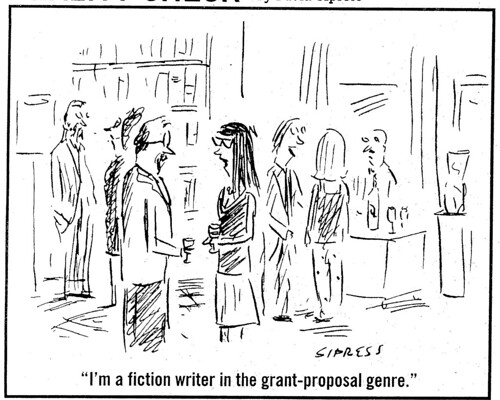
\includegraphics[width=0.7\textwidth]{fiction.png}};
      \end{tikzpicture}
    }{
    \tableofcontents[currentsection]
    }
  \end{frame}
}

\section{Introduction}

\begin{frame}{Probabilistic Relational Models}
  \begin{block}{Markov Logic Network (\cite{DBLP:journals/ml/RichardsonD06})}
    \vspace*{-\baselineskip}\setlength\belowdisplayshortskip{0pt}
    \begin{align*}
      0.7 &\quad \forall x \forall y \forall z \; \mathtt{Friends}(x, y) \land \mathtt{Friends}(y, z) \Rightarrow \mathtt{Friends}(x, z) \\
      2.3 &\quad \forall x \; \lnot\exists y \; \mathtt{Friends}(x, y) \Rightarrow \mathtt{Smokes}(x) \\
      1.5 &\quad \forall x \; \mathtt{Smokes}(x) \Rightarrow \mathtt{Cancer}(x) \\
      1.1 &\quad \forall x \forall y \; \mathtt{Friends}(x, y) \Rightarrow (\mathtt{Smokes}(x) \Leftrightarrow \mathtt{Smokes}(y))
    \end{align*}
  \end{block}
\end{frame}

\begin{frame}{Probabilistic Relational Models}
  \begin{block}{ProbLog (\cite{DBLP:conf/ijcai/RaedtKT07})}
    \vspace*{-\baselineskip}\setlength\belowdisplayshortskip{0pt}
    \begin{align*}
      1.0 &\prob \mathtt{likes}(X, Y) \ifff \mathtt{friendOf}(X, Y). \\
      0.8 &\prob \mathtt{likes}(X, Y) \ifff \mathtt{friendOf}(X, Z), \mathtt{likes}(Z, Y). \\
      0.5 &\prob \mathtt{friendOf}(\mathit{john}, \mathit{mary}). \\
      0.5 &\prob \mathtt{friendOf}(\mathit{mary}, \mathit{pedro}). \\
      0.5 &\prob \mathtt{friendOf}(\mathit{mary}, \mathit{tom}). \\
      0.5 &\prob \mathtt{friendOf}(\mathit{pedro}, \mathit{tom}).
    \end{align*}
  \end{block}
\end{frame}

\begin{frame}{Probabilistic Relational Models}
  \begin{itemize}
  \item What do these models have in common?
  \item When performing inference...
    \begin{itemize}
    \item do we have to consider every detail?
    \item what makes inference challenging?
    \item can we do any better?
    \end{itemize}
  \item How can we learn PRMs from data?
  \end{itemize}
\end{frame}

\begin{frame}{Applications}
  \begin{columns}
    \begin{column}{0.5\textwidth}
      \centering
      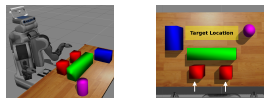
\includegraphics[width=\textwidth,height=0.5\textheight,keepaspectratio]{application_robots.jpg}
      \\[-7pt]
      {\tiny \cite{DBLP:conf/iros/MoldovanR14}}
      \vfill
      \null
      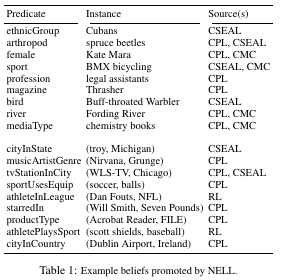
\includegraphics[width=\textwidth,height=0.5\textheight,keepaspectratio]{application_nell.jpg}
      \\[-7pt]
      {\tiny \cite{DBLP:conf/aaai/CarlsonBKSHM10}}
    \end{column}
    \begin{column}{0.5\textwidth}
      \centering
      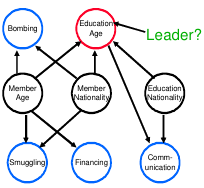
\includegraphics[width=\textwidth,height=0.4\textheight,keepaspectratio]{application_criminal.jpg}
      \\[-7pt]
      {\tiny \cite{DBLP:conf/sdm/DelaneyFCWJ10}}
      \vfill
      \null
      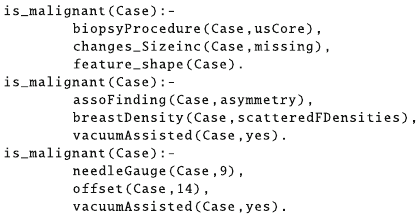
\includegraphics[width=\textwidth,height=0.5\textheight,keepaspectratio]{application_cancer.jpg}
      \\[-7pt]
      {\tiny \cite{DBLP:conf/ilp/Corte-RealD017}}
    \end{column}
  \end{columns}
\end{frame}

\section{Equivalence}

\begin{frame}
  \begin{columns}
    \begin{column}{0.5\textwidth}
      \begin{alertblock}{}
        \vspace*{-1.5\baselineskip}\setlength\belowdisplayshortskip{0pt}
        \begin{gather*}
          \mathtt{Husband}(\mathit{joffrey}, \mathit{margaery}) \\
          \mathtt{Husband}(\mathit{tommen}, \mathit{margaery}) \\
          \mathtt{Husband}(\mathit{renly}, \mathit{margaery}) \\
          \mathtt{Parent}(\mathit{cersei}, \mathit{joffrey}) \\
          \mathtt{Parent}(\mathit{cersei}, \mathit{myrcella}) \\
          \mathtt{Parent}(\mathit{cersei}, \mathit{tommen}) \\
          \mathtt{Parent}(\mathit{tywin}, \mathit{cersei})
        \end{gather*}
        \vspace*{-1.5\baselineskip}\setlength\belowdisplayshortskip{0pt}
      \end{alertblock}
    \end{column}
    \begin{column}{0.5\textwidth}
      \begin{exampleblock}{}<2->
        \vspace*{-1.5\baselineskip}\setlength\belowdisplayshortskip{0pt}
        \begin{gather*}
          \mathtt{Female}(\mathit{cersei}), \\
          \mathtt{Female}(\mathit{margaery}), \\
          \mathtt{Female}(\mathit{myrcella})
        \end{gather*}
        \vspace*{-1.5\baselineskip}\setlength\belowdisplayshortskip{0pt}
      \end{exampleblock}
    \end{column}
  \end{columns}
  \begin{block}{}<3->
    \vspace*{-1.5\baselineskip}\setlength\belowdisplayshortskip{0pt}
    \begin{align*}
      \mathtt{Female}(X) &\ifff \mathtt{Husband}(\mathit{joffrey}, X). \\
      \mathtt{Female}(X) &\ifff \mathtt{Parent}(X, \mathit{joffrey}). \\
      \mathtt{Female}(X) &\ifff \mathtt{Parent}(\mathit{cersei}, X), \neg\mathtt{Husband}(X, \mathit{margaery}).
    \end{align*}
    \vspace*{-1.5\baselineskip}\setlength\belowdisplayshortskip{0pt}
  \end{block}
\end{frame}

\begin{frame}{Main Results}
  \begin{definition}[Equivalence]
    Two $n$-tuples of constants $a$ and $b$ are \alert{equivalent} if
    \[
      (\mathtt{P} \circ \rho)(a) = (\mathtt{P} \circ \rho)(b)
    \]
    for all atoms $\mathtt{P} \circ \rho$ acting on $n$ variables.
  \end{definition}
  \pause
  \begin{theorem}
    There is a logic program $\mathcal{L}\colon \mathcal{KB}(P_1, C) \to
    \mathcal{KB}(P_2, C)$ such that $\mathcal{L}(\Delta_1) = \Delta_2$ if and
    only if ${\sim_{\Delta_2}}$ is coarser than ${\sim_{\Delta_1}}$.
  \end{theorem}
\end{frame}

\section{Random Programs}

\begin{frame}{What Characterises a Program?}
  \begin{columns}
    \hspace*{-0.7cm}\begin{column}{0.75\textwidth}
      \begin{empheq}[left =\onslide<6->{\color{color5}\empheqlbrace}]{equation}
        \begin{align*}
          \textcolor<5->{color4}{1.0} &\prob \textcolor<2->{color1}{\mathtt{likes}}(\textcolor<3->{color2}{X}, \textcolor<3->{color2}{Y}) \ifff \textcolor<2->{color1}{\mathtt{friendOf}}(\textcolor<3->{color2}{X}, \textcolor<3->{color2}{Y}). \\
          \textcolor<5->{color4}{0.8} &\prob \textcolor<2->{color1}{\mathtt{likes}}(\textcolor<3->{color2}{X}, \textcolor<3->{color2}{Y}) \ifff \tikz \coordinate (start);\textcolor<2->{color1}{\mathtt{friendOf}}(\textcolor<3->{color2}{X}, \textcolor<3->{color2}{Z}), \textcolor<2->{color1}{\mathtt{likes}}(\textcolor<3->{color2}{Z}, \textcolor<3->{color2}{Y})\tikz \coordinate (end);. \\
          \textcolor<5->{color4}{0.5} &\prob \textcolor<2->{color1}{\mathtt{friendOf}}(\textcolor<4->{color3}{\mathit{john}}, \textcolor<4->{color3}{\mathit{mary}}). \\
          \textcolor<5->{color4}{0.5} &\prob \textcolor<2->{color1}{\mathtt{friendOf}}(\textcolor<4->{color3}{\mathit{mary}}, \textcolor<4->{color3}{\mathit{pedro}}). \\
          \textcolor<5->{color4}{0.5} &\prob \textcolor<2->{color1}{\mathtt{friendOf}}(\textcolor<4->{color3}{\mathit{mary}}, \textcolor<4->{color3}{\mathit{tom}}). \\
          \textcolor<5->{color4}{0.5} &\prob \textcolor<2->{color1}{\mathtt{friendOf}}(\textcolor<4->{color3}{\mathit{pedro}}, \textcolor<4->{color3}{\mathit{tom}}).
        \end{align*}
      \end{empheq}
    \end{column}
    \begin{column}{0.25\textwidth}
      \begin{itemize}
      \item[\textcolor{color1}{\textbullet}]<2-> predicates, arities
      \item[\textcolor{color2}{\textbullet}]<3-> variables
      \item[\textcolor{color3}{\textbullet}]<4-> constants
      \item[\textcolor{color4}{\textbullet}]<5-> probabilities
      \item[\textcolor{color5}{\textbullet}]<6-> length
      \item[\textcolor{color6}{\textbullet}]<7-> complexity
      \end{itemize}
    \end{column}
  \end{columns}
  \onslide<7->{
    \begin{tikzpicture}[overlay]
      \draw [decorate,decoration={brace,amplitude=10pt,mirror},color=color6] (start) -- (end);
    \end{tikzpicture}
  }
  \begin{columns}
    \begin{column}{0.27\textwidth}
      \onslide<9->{
        Also:
        \begin{itemize}
        \item cyclicity
        \item (conditional) independence
        \item required subformulas
        \end{itemize}
      }
    \end{column}
    \begin{column}{0.53\textwidth}
      \onslide<8->{
        \begin{tikzpicture}
          \node[draw,circle,gray,text=black] (and) at (0, 0) {$\land$};
          \node[draw,gray,text=black] (friendOf) at (-1.5, -1) {$\textcolor{color1}{\mathtt{friendOf}}\textcolor{black}{(}\textcolor<3->{color2}{X}\textcolor{black}{,}\,\textcolor<3->{color2}{Z}\textcolor{black}{)}$};
          \node[draw,gray,text=black] (likes) at (1.5, -1) {$\textcolor{color1}{\mathtt{likes}}\textcolor{black}{(}\textcolor<3->{color2}{Z}\textcolor{black}{,}\,\textcolor<3->{color2}{Y}\textcolor{black}{)}$};
          \draw[gray] (and) -- (friendOf);
          \draw[gray] (and) -- (likes);
        \end{tikzpicture}
      }
    \end{column}
    \begin{column}{0.2\textwidth}
      \onslide<10->{
        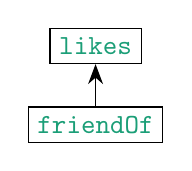
\begin{tikzpicture}
          \node[draw] (likes) {\textcolor{color1}{$\mathtt{likes}$}};
          \node[draw,below of = likes] (friendOf) {\textcolor{color1}{$\mathtt{friendOf}$}};
          \draw[-{Stealth[scale=1.5]}] (friendOf) -- (likes);
        \end{tikzpicture}
      }
    \end{column}
  \end{columns}
\end{frame}

\begin{frame}{What Programs Are Hard to Generate?}
  \begin{figure}
    \centering
    % Created by tikzDevice version 0.12.3.1 on 2022-06-27 14:20:09
% !TEX encoding = UTF-8 Unicode
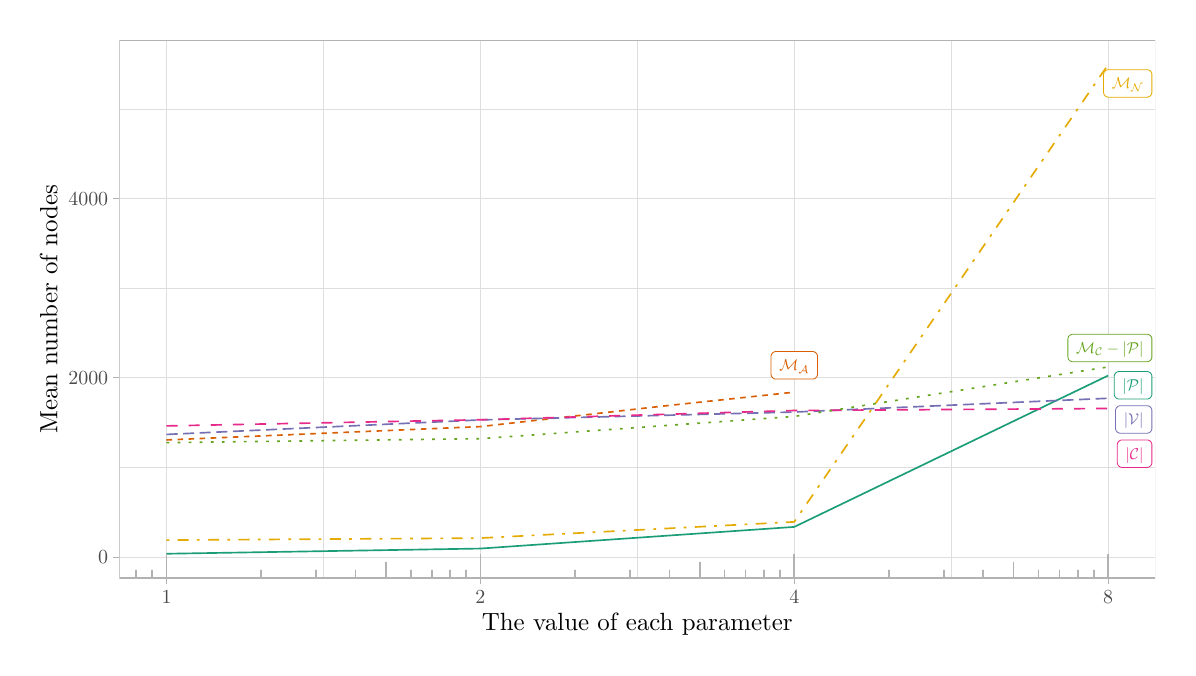
\begin{tikzpicture}[x=1pt,y=1pt]
\definecolor{fillColor}{RGB}{255,255,255}
\path[use as bounding box,fill=fillColor,fill opacity=0.00] (0,0) rectangle (411.94,224.04);
\begin{scope}
\path[clip] (  0.00,  0.00) rectangle (411.94,224.04);
\definecolor{drawColor}{RGB}{255,255,255}
\definecolor{fillColor}{RGB}{255,255,255}

\path[draw=drawColor,line width= 0.5pt,line join=round,line cap=round,fill=fillColor] (  0.00,  0.00) rectangle (411.94,224.04);
\end{scope}
\begin{scope}
\path[clip] ( 33.14, 25.11) rectangle (407.44,219.54);
\definecolor{fillColor}{RGB}{255,255,255}

\path[fill=fillColor] ( 33.14, 25.11) rectangle (407.44,219.54);
\definecolor{drawColor}{gray}{0.87}

\path[draw=drawColor,line width= 0.1pt,line join=round] ( 33.14, 65.17) --
	(407.44, 65.17);

\path[draw=drawColor,line width= 0.1pt,line join=round] ( 33.14,129.92) --
	(407.44,129.92);

\path[draw=drawColor,line width= 0.1pt,line join=round] ( 33.14,194.66) --
	(407.44,194.66);

\path[draw=drawColor,line width= 0.1pt,line join=round] (106.87, 25.11) --
	(106.87,219.54);

\path[draw=drawColor,line width= 0.1pt,line join=round] (220.29, 25.11) --
	(220.29,219.54);

\path[draw=drawColor,line width= 0.1pt,line join=round] (333.71, 25.11) --
	(333.71,219.54);

\path[draw=drawColor,line width= 0.2pt,line join=round] ( 33.14, 32.80) --
	(407.44, 32.80);

\path[draw=drawColor,line width= 0.2pt,line join=round] ( 33.14, 97.54) --
	(407.44, 97.54);

\path[draw=drawColor,line width= 0.2pt,line join=round] ( 33.14,162.29) --
	(407.44,162.29);

\path[draw=drawColor,line width= 0.2pt,line join=round] ( 50.16, 25.11) --
	( 50.16,219.54);

\path[draw=drawColor,line width= 0.2pt,line join=round] (163.58, 25.11) --
	(163.58,219.54);

\path[draw=drawColor,line width= 0.2pt,line join=round] (277.00, 25.11) --
	(277.00,219.54);

\path[draw=drawColor,line width= 0.2pt,line join=round] (390.43, 25.11) --
	(390.43,219.54);
\definecolor{drawColor}{RGB}{27,158,119}

\path[draw=drawColor,line width= 0.6pt,line join=round] ( 50.16, 33.94) --
	(163.58, 35.82) --
	(277.00, 43.64) --
	(390.43, 98.33);
\definecolor{drawColor}{RGB}{217,95,2}

\path[draw=drawColor,line width= 0.6pt,dash pattern=on 2pt off 2pt ,line join=round] ( 50.16, 75.06) --
	(163.58, 79.89) --
	(229.93, 87.34) --
	(277.00, 92.33);
\definecolor{drawColor}{RGB}{117,112,179}

\path[draw=drawColor,line width= 0.6pt,dash pattern=on 4pt off 2pt ,line join=round] ( 50.16, 77.05) --
	(163.58, 82.31) --
	(277.00, 85.14) --
	(390.43, 90.12);
\definecolor{drawColor}{RGB}{231,41,138}

\path[draw=drawColor,line width= 0.6pt,dash pattern=on 4pt off 4pt ,line join=round] ( 50.16, 80.14) --
	(163.58, 82.36) --
	(277.00, 85.70) --
	(390.43, 86.43);
\definecolor{drawColor}{RGB}{102,166,30}

\path[draw=drawColor,line width= 0.6pt,dash pattern=on 1pt off 3pt ,line join=round] ( 50.16, 74.09) --
	(163.58, 75.52) --
	(277.00, 83.56) --
	(390.43,101.45);
\definecolor{drawColor}{RGB}{230,171,2}

\path[draw=drawColor,line width= 0.6pt,dash pattern=on 1pt off 3pt on 4pt off 3pt ,line join=round] ( 50.16, 38.87) --
	(163.58, 39.60) --
	(277.00, 45.46) --
	(390.43,210.70);
\end{scope}
\begin{scope}
\path[clip] ( 33.14, 25.11) rectangle (407.44,219.54);

\path[] (399.52, 75.07) -- (390.90, 85.83);
\definecolor{drawColor}{RGB}{27,158,119}
\definecolor{fillColor}{RGB}{255,255,255}

\path[draw=drawColor,line width= 0.3pt,line join=round,line cap=round,fill=fillColor] (394.43, 89.84) --
	(404.43, 89.84) --
	(404.35, 89.85) --
	(404.65, 89.86) --
	(404.93, 89.92) --
	(405.20, 90.02) --
	(405.45, 90.16) --
	(405.68, 90.35) --
	(405.87, 90.57) --
	(406.03, 90.81) --
	(406.14, 91.08) --
	(406.21, 91.36) --
	(406.23, 91.65) --
	(406.23, 91.65) --
	(406.23, 97.98) --
	(406.23, 97.98) --
	(406.21, 98.27) --
	(406.14, 98.55) --
	(406.03, 98.82) --
	(405.87, 99.06) --
	(405.68, 99.28) --
	(405.45, 99.47) --
	(405.20, 99.61) --
	(404.93, 99.71) --
	(404.65, 99.77) --
	(404.43, 99.79) --
	(394.43, 99.79) --
	(394.65, 99.77) --
	(394.36, 99.78) --
	(394.07, 99.75) --
	(393.79, 99.67) --
	(393.53, 99.54) --
	(393.29, 99.38) --
	(393.08, 99.18) --
	(392.90, 98.94) --
	(392.77, 98.69) --
	(392.68, 98.41) --
	(392.63, 98.12) --
	(392.62, 97.98) --
	(392.62, 91.65) --
	(392.63, 91.80) --
	(392.63, 91.51) --
	(392.68, 91.22) --
	(392.77, 90.94) --
	(392.90, 90.68) --
	(393.08, 90.45) --
	(393.29, 90.25) --
	(393.53, 90.09) --
	(393.79, 89.96) --
	(394.07, 89.88) --
	(394.36, 89.85) --
	cycle;
\end{scope}
\begin{scope}
\path[clip] ( 33.14, 25.11) rectangle (407.44,219.54);
\definecolor{drawColor}{RGB}{27,158,119}

\node[text=drawColor,anchor=base,inner sep=0pt, outer sep=0pt, scale=  0.57] at (399.43, 92.86) {$|\mathcal{P}|$};
\definecolor{drawColor}{RGB}{117,112,179}
\definecolor{fillColor}{RGB}{255,255,255}

\path[draw=drawColor,line width= 0.3pt,line join=round,line cap=round,fill=fillColor] (394.90, 77.50) --
	(404.43, 77.50) --
	(404.35, 77.50) --
	(404.65, 77.51) --
	(404.93, 77.57) --
	(405.20, 77.67) --
	(405.45, 77.82) --
	(405.68, 78.00) --
	(405.87, 78.22) --
	(406.03, 78.46) --
	(406.14, 78.73) --
	(406.21, 79.01) --
	(406.23, 79.30) --
	(406.23, 79.30) --
	(406.23, 85.63) --
	(406.23, 85.63) --
	(406.21, 85.92) --
	(406.14, 86.20) --
	(406.03, 86.47) --
	(405.87, 86.72) --
	(405.68, 86.94) --
	(405.45, 87.12) --
	(405.20, 87.26) --
	(404.93, 87.37) --
	(404.65, 87.43) --
	(404.43, 87.44) --
	(394.90, 87.44) --
	(395.12, 87.43) --
	(394.83, 87.44) --
	(394.54, 87.40) --
	(394.26, 87.32) --
	(394.00, 87.20) --
	(393.76, 87.03) --
	(393.55, 86.83) --
	(393.37, 86.60) --
	(393.24, 86.34) --
	(393.15, 86.06) --
	(393.10, 85.78) --
	(393.09, 85.63) --
	(393.09, 79.30) --
	(393.10, 79.45) --
	(393.10, 79.16) --
	(393.15, 78.87) --
	(393.24, 78.60) --
	(393.37, 78.34) --
	(393.55, 78.11) --
	(393.76, 77.90) --
	(394.00, 77.74) --
	(394.26, 77.61) --
	(394.54, 77.53) --
	(394.83, 77.50) --
	cycle;
\end{scope}
\begin{scope}
\path[clip] ( 33.14, 25.11) rectangle (407.44,219.54);
\definecolor{drawColor}{RGB}{117,112,179}

\node[text=drawColor,anchor=base,inner sep=0pt, outer sep=0pt, scale=  0.57] at (399.66, 80.51) {$|\mathcal{V}|$};
\definecolor{drawColor}{RGB}{231,41,138}
\definecolor{fillColor}{RGB}{255,255,255}

\path[draw=drawColor,line width= 0.3pt,line join=round,line cap=round,fill=fillColor] (395.53, 65.13) --
	(404.43, 65.13) --
	(404.35, 65.13) --
	(404.65, 65.14) --
	(404.93, 65.20) --
	(405.20, 65.30) --
	(405.45, 65.45) --
	(405.68, 65.63) --
	(405.87, 65.85) --
	(406.03, 66.09) --
	(406.14, 66.36) --
	(406.21, 66.64) --
	(406.23, 66.93) --
	(406.23, 66.93) --
	(406.23, 73.26) --
	(406.23, 73.26) --
	(406.21, 73.55) --
	(406.14, 73.83) --
	(406.03, 74.10) --
	(405.87, 74.35) --
	(405.68, 74.56) --
	(405.45, 74.75) --
	(405.20, 74.89) --
	(404.93, 75.00) --
	(404.65, 75.05) --
	(404.43, 75.07) --
	(395.53, 75.07) --
	(395.75, 75.05) --
	(395.46, 75.07) --
	(395.17, 75.03) --
	(394.89, 74.95) --
	(394.63, 74.83) --
	(394.39, 74.66) --
	(394.18, 74.46) --
	(394.00, 74.23) --
	(393.87, 73.97) --
	(393.77, 73.69) --
	(393.73, 73.41) --
	(393.72, 73.26) --
	(393.72, 66.93) --
	(393.73, 67.08) --
	(393.73, 66.79) --
	(393.77, 66.50) --
	(393.87, 66.22) --
	(394.00, 65.97) --
	(394.18, 65.73) --
	(394.39, 65.53) --
	(394.63, 65.37) --
	(394.89, 65.24) --
	(395.17, 65.16) --
	(395.46, 65.13) --
	cycle;
\end{scope}
\begin{scope}
\path[clip] ( 33.14, 25.11) rectangle (407.44,219.54);
\definecolor{drawColor}{RGB}{231,41,138}

\node[text=drawColor,anchor=base,inner sep=0pt, outer sep=0pt, scale=  0.57] at (399.98, 68.14) {$|\mathcal{C}|$};
\definecolor{drawColor}{RGB}{102,166,30}
\definecolor{fillColor}{RGB}{255,255,255}

\path[draw=drawColor,line width= 0.3pt,line join=round,line cap=round,fill=fillColor] (377.69,103.32) --
	(404.43,103.32) --
	(404.35,103.32) --
	(404.65,103.33) --
	(404.93,103.39) --
	(405.20,103.49) --
	(405.45,103.64) --
	(405.68,103.82) --
	(405.87,104.04) --
	(406.03,104.29) --
	(406.14,104.55) --
	(406.21,104.84) --
	(406.23,105.13) --
	(406.23,105.13) --
	(406.23,111.45) --
	(406.23,111.45) --
	(406.21,111.74) --
	(406.14,112.03) --
	(406.03,112.29) --
	(405.87,112.54) --
	(405.68,112.76) --
	(405.45,112.94) --
	(405.20,113.09) --
	(404.93,113.19) --
	(404.65,113.25) --
	(404.43,113.26) --
	(377.69,113.26) --
	(377.90,113.25) --
	(377.61,113.26) --
	(377.32,113.22) --
	(377.05,113.14) --
	(376.78,113.02) --
	(376.54,112.85) --
	(376.33,112.65) --
	(376.16,112.42) --
	(376.02,112.16) --
	(375.93,111.89) --
	(375.89,111.60) --
	(375.88,111.45) --
	(375.88,105.13) --
	(375.89,105.27) --
	(375.89,104.98) --
	(375.93,104.69) --
	(376.02,104.42) --
	(376.16,104.16) --
	(376.33,103.93) --
	(376.54,103.73) --
	(376.78,103.56) --
	(377.05,103.44) --
	(377.32,103.36) --
	(377.61,103.32) --
	cycle;
\end{scope}
\begin{scope}
\path[clip] ( 33.14, 25.11) rectangle (407.44,219.54);
\definecolor{drawColor}{RGB}{102,166,30}

\node[text=drawColor,anchor=base,inner sep=0pt, outer sep=0pt, scale=  0.57] at (391.06,106.33) {$\mathcal{M}_{\mathcal{C}}-|\mathcal{P}|$};
\definecolor{drawColor}{RGB}{230,171,2}
\definecolor{fillColor}{RGB}{255,255,255}

\path[draw=drawColor,line width= 0.3pt,line join=round,line cap=round,fill=fillColor] (390.57,198.92) --
	(404.43,198.92) --
	(404.35,198.92) --
	(404.65,198.94) --
	(404.93,198.99) --
	(405.20,199.10) --
	(405.45,199.24) --
	(405.68,199.43) --
	(405.87,199.64) --
	(406.03,199.89) --
	(406.14,200.16) --
	(406.21,200.44) --
	(406.23,200.73) --
	(406.23,200.73) --
	(406.23,207.06) --
	(406.23,207.06) --
	(406.21,207.35) --
	(406.14,207.63) --
	(406.03,207.90) --
	(405.87,208.14) --
	(405.68,208.36) --
	(405.45,208.54) --
	(405.20,208.69) --
	(404.93,208.79) --
	(404.65,208.85) --
	(404.43,208.86) --
	(390.57,208.86) --
	(390.79,208.85) --
	(390.50,208.86) --
	(390.21,208.83) --
	(389.93,208.75) --
	(389.67,208.62) --
	(389.43,208.46) --
	(389.22,208.26) --
	(389.05,208.02) --
	(388.91,207.77) --
	(388.82,207.49) --
	(388.77,207.20) --
	(388.77,207.06) --
	(388.77,200.73) --
	(388.77,200.87) --
	(388.77,200.58) --
	(388.82,200.30) --
	(388.91,200.02) --
	(389.05,199.76) --
	(389.22,199.53) --
	(389.43,199.33) --
	(389.67,199.16) --
	(389.93,199.04) --
	(390.21,198.96) --
	(390.50,198.92) --
	cycle;
\end{scope}
\begin{scope}
\path[clip] ( 33.14, 25.11) rectangle (407.44,219.54);
\definecolor{drawColor}{RGB}{230,171,2}

\node[text=drawColor,anchor=base,inner sep=0pt, outer sep=0pt, scale=  0.57] at (397.50,201.93) {$\mathcal{M}_{\mathcal{N}}$};
\end{scope}
\begin{scope}
\path[clip] ( 33.14, 25.11) rectangle (407.44,219.54);
\definecolor{drawColor}{RGB}{217,95,2}
\definecolor{fillColor}{RGB}{255,255,255}

\path[draw=drawColor,line width= 0.3pt,line join=round,line cap=round,fill=fillColor] (270.41, 97.07) --
	(283.59, 97.07) --
	(283.52, 97.07) --
	(283.81, 97.09) --
	(284.10, 97.14) --
	(284.37, 97.25) --
	(284.62, 97.39) --
	(284.85, 97.58) --
	(285.04, 97.79) --
	(285.19, 98.04) --
	(285.31, 98.31) --
	(285.38, 98.59) --
	(285.40, 98.88) --
	(285.40, 98.88) --
	(285.40,105.21) --
	(285.40,105.21) --
	(285.38,105.50) --
	(285.31,105.78) --
	(285.19,106.05) --
	(285.04,106.29) --
	(284.85,106.51) --
	(284.62,106.69) --
	(284.37,106.84) --
	(284.10,106.94) --
	(283.81,107.00) --
	(283.59,107.01) --
	(270.41,107.01) --
	(270.63,107.00) --
	(270.34,107.01) --
	(270.05,106.98) --
	(269.77,106.90) --
	(269.51,106.77) --
	(269.27,106.61) --
	(269.06,106.41) --
	(268.88,106.17) --
	(268.75,105.92) --
	(268.66,105.64) --
	(268.61,105.35) --
	(268.60,105.21) --
	(268.60, 98.88) --
	(268.61, 99.02) --
	(268.61, 98.73) --
	(268.66, 98.45) --
	(268.75, 98.17) --
	(268.88, 97.91) --
	(269.06, 97.68) --
	(269.27, 97.48) --
	(269.51, 97.31) --
	(269.77, 97.19) --
	(270.05, 97.11) --
	(270.34, 97.07) --
	cycle;
\end{scope}
\begin{scope}
\path[clip] ( 33.14, 25.11) rectangle (407.44,219.54);
\definecolor{drawColor}{RGB}{217,95,2}

\node[text=drawColor,anchor=base,inner sep=0pt, outer sep=0pt, scale=  0.57] at (277.00,100.08) {$\mathcal{M}_{\mathcal{A}}$};
\definecolor{drawColor}{gray}{0.70}

\path[draw=drawColor,line width= 0.6pt,line join=round,line cap=round] ( 39.17, 25.11) -- ( 39.17, 27.95);

\path[draw=drawColor,line width= 0.6pt,line join=round,line cap=round] ( 44.97, 25.11) -- ( 44.97, 27.95);

\path[draw=drawColor,line width= 0.6pt,line join=round,line cap=round] ( 50.16, 25.11) -- ( 50.16, 33.64);

\path[draw=drawColor,line width= 0.6pt,line join=round,line cap=round] ( 84.30, 25.11) -- ( 84.30, 27.95);

\path[draw=drawColor,line width= 0.6pt,line join=round,line cap=round] (104.27, 25.11) -- (104.27, 27.95);

\path[draw=drawColor,line width= 0.6pt,line join=round,line cap=round] (118.45, 25.11) -- (118.45, 27.95);

\path[draw=drawColor,line width= 0.6pt,line join=round,line cap=round] (129.44, 25.11) -- (129.44, 30.80);

\path[draw=drawColor,line width= 0.6pt,line join=round,line cap=round] (138.42, 25.11) -- (138.42, 27.95);

\path[draw=drawColor,line width= 0.6pt,line join=round,line cap=round] (146.01, 25.11) -- (146.01, 27.95);

\path[draw=drawColor,line width= 0.6pt,line join=round,line cap=round] (152.59, 25.11) -- (152.59, 27.95);

\path[draw=drawColor,line width= 0.6pt,line join=round,line cap=round] (158.39, 25.11) -- (158.39, 27.95);

\path[draw=drawColor,line width= 0.6pt,line join=round,line cap=round] (163.58, 25.11) -- (163.58, 33.64);

\path[draw=drawColor,line width= 0.6pt,line join=round,line cap=round] (197.72, 25.11) -- (197.72, 27.95);

\path[draw=drawColor,line width= 0.6pt,line join=round,line cap=round] (217.70, 25.11) -- (217.70, 27.95);

\path[draw=drawColor,line width= 0.6pt,line join=round,line cap=round] (231.87, 25.11) -- (231.87, 27.95);

\path[draw=drawColor,line width= 0.6pt,line join=round,line cap=round] (242.86, 25.11) -- (242.86, 30.80);

\path[draw=drawColor,line width= 0.6pt,line join=round,line cap=round] (251.84, 25.11) -- (251.84, 27.95);

\path[draw=drawColor,line width= 0.6pt,line join=round,line cap=round] (259.43, 25.11) -- (259.43, 27.95);

\path[draw=drawColor,line width= 0.6pt,line join=round,line cap=round] (266.01, 25.11) -- (266.01, 27.95);

\path[draw=drawColor,line width= 0.6pt,line join=round,line cap=round] (271.81, 25.11) -- (271.81, 27.95);

\path[draw=drawColor,line width= 0.6pt,line join=round,line cap=round] (277.00, 25.11) -- (277.00, 33.64);

\path[draw=drawColor,line width= 0.6pt,line join=round,line cap=round] (311.15, 25.11) -- (311.15, 27.95);

\path[draw=drawColor,line width= 0.6pt,line join=round,line cap=round] (331.12, 25.11) -- (331.12, 27.95);

\path[draw=drawColor,line width= 0.6pt,line join=round,line cap=round] (345.29, 25.11) -- (345.29, 27.95);

\path[draw=drawColor,line width= 0.6pt,line join=round,line cap=round] (356.28, 25.11) -- (356.28, 30.80);

\path[draw=drawColor,line width= 0.6pt,line join=round,line cap=round] (365.26, 25.11) -- (365.26, 27.95);

\path[draw=drawColor,line width= 0.6pt,line join=round,line cap=round] (372.86, 25.11) -- (372.86, 27.95);

\path[draw=drawColor,line width= 0.6pt,line join=round,line cap=round] (379.43, 25.11) -- (379.43, 27.95);

\path[draw=drawColor,line width= 0.6pt,line join=round,line cap=round] (385.24, 25.11) -- (385.24, 27.95);

\path[draw=drawColor,line width= 0.6pt,line join=round,line cap=round] (390.43, 25.11) -- (390.43, 33.64);

\path[draw=drawColor,line width= 0.5pt,line join=round,line cap=round] ( 33.14, 25.11) rectangle (407.44,219.54);
\end{scope}
\begin{scope}
\path[clip] (  0.00,  0.00) rectangle (411.94,224.04);
\definecolor{drawColor}{gray}{0.30}

\node[text=drawColor,anchor=base east,inner sep=0pt, outer sep=0pt, scale=  0.72] at ( 29.09, 30.32) {0};

\node[text=drawColor,anchor=base east,inner sep=0pt, outer sep=0pt, scale=  0.72] at ( 29.09, 95.06) {2000};

\node[text=drawColor,anchor=base east,inner sep=0pt, outer sep=0pt, scale=  0.72] at ( 29.09,159.81) {4000};
\end{scope}
\begin{scope}
\path[clip] (  0.00,  0.00) rectangle (411.94,224.04);
\definecolor{drawColor}{gray}{0.70}

\path[draw=drawColor,line width= 0.2pt,line join=round] ( 30.89, 32.80) --
	( 33.14, 32.80);

\path[draw=drawColor,line width= 0.2pt,line join=round] ( 30.89, 97.54) --
	( 33.14, 97.54);

\path[draw=drawColor,line width= 0.2pt,line join=round] ( 30.89,162.29) --
	( 33.14,162.29);
\end{scope}
\begin{scope}
\path[clip] (  0.00,  0.00) rectangle (411.94,224.04);
\definecolor{drawColor}{gray}{0.70}

\path[draw=drawColor,line width= 0.2pt,line join=round] ( 50.16, 22.86) --
	( 50.16, 25.11);

\path[draw=drawColor,line width= 0.2pt,line join=round] (163.58, 22.86) --
	(163.58, 25.11);

\path[draw=drawColor,line width= 0.2pt,line join=round] (277.00, 22.86) --
	(277.00, 25.11);

\path[draw=drawColor,line width= 0.2pt,line join=round] (390.43, 22.86) --
	(390.43, 25.11);
\end{scope}
\begin{scope}
\path[clip] (  0.00,  0.00) rectangle (411.94,224.04);
\definecolor{drawColor}{gray}{0.30}

\node[text=drawColor,anchor=base,inner sep=0pt, outer sep=0pt, scale=  0.72] at ( 50.16, 16.10) {1};

\node[text=drawColor,anchor=base,inner sep=0pt, outer sep=0pt, scale=  0.72] at (163.58, 16.10) {2};

\node[text=drawColor,anchor=base,inner sep=0pt, outer sep=0pt, scale=  0.72] at (277.00, 16.10) {4};

\node[text=drawColor,anchor=base,inner sep=0pt, outer sep=0pt, scale=  0.72] at (390.43, 16.10) {8};
\end{scope}
\begin{scope}
\path[clip] (  0.00,  0.00) rectangle (411.94,224.04);
\definecolor{drawColor}{RGB}{0,0,0}

\node[text=drawColor,anchor=base,inner sep=0pt, outer sep=0pt, scale=  0.90] at (220.29,  6.25) {The value of each parameter};
\end{scope}
\begin{scope}
\path[clip] (  0.00,  0.00) rectangle (411.94,224.04);
\definecolor{drawColor}{RGB}{0,0,0}

\node[text=drawColor,rotate= 90.00,anchor=base,inner sep=0pt, outer sep=0pt, scale=  0.90] at ( 10.70,122.32) {Mean number of nodes};
\end{scope}
\end{tikzpicture}

  \end{figure}
\end{frame}

\begin{frame}{What Programs Are Hard to Generate?}
  \begin{figure}
    \centering
    \resizebox{\linewidth}{!}{% Created by tikzDevice version 0.12.3 on 2020-01-25 19:15:40
% !TEX encoding = UTF-8 Unicode
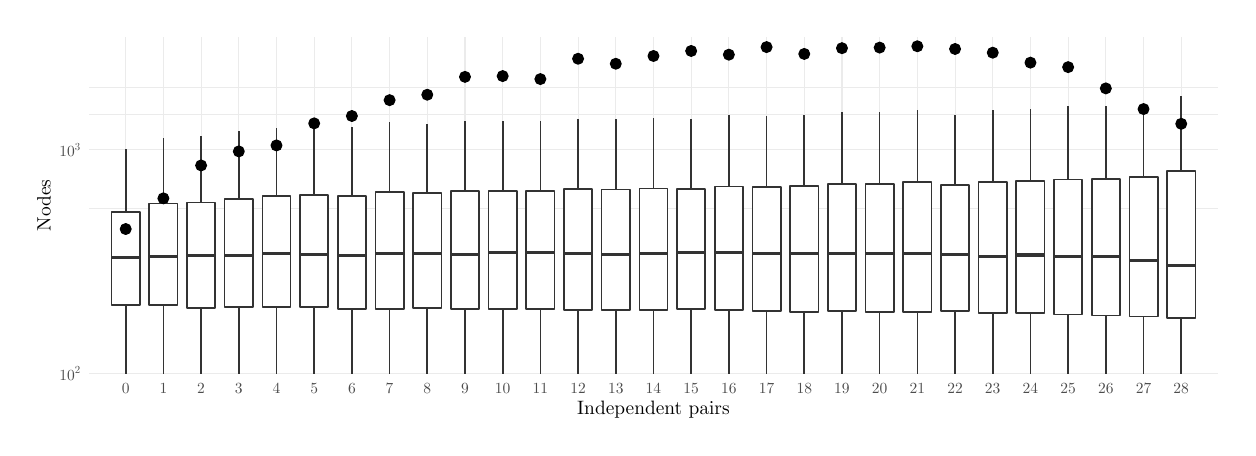
\begin{tikzpicture}[x=1pt,y=1pt]
\definecolor{fillColor}{RGB}{255,255,255}
\path[use as bounding box,fill=fillColor,fill opacity=0.00] (0,0) rectangle (433.62,144.54);
\begin{scope}
\path[clip] ( 22.14, 19.53) rectangle (430.12,141.04);
\definecolor{drawColor}{gray}{0.92}

\path[draw=drawColor,line width= 0.2pt,line join=round] ( 22.14, 79.39) --
	(430.12, 79.39);

\path[draw=drawColor,line width= 0.2pt,line join=round] ( 22.14,113.42) --
	(430.12,113.42);

\path[draw=drawColor,line width= 0.2pt,line join=round] ( 22.14,122.92) --
	(430.12,122.92);

\path[draw=drawColor,line width= 0.4pt,line join=round] ( 22.14, 19.53) --
	(430.12, 19.53);

\path[draw=drawColor,line width= 0.4pt,line join=round] ( 22.14,100.38) --
	(430.12,100.38);

\path[draw=drawColor,line width= 0.4pt,line join=round] ( 35.42, 19.53) --
	( 35.42,141.04);

\path[draw=drawColor,line width= 0.4pt,line join=round] ( 49.04, 19.53) --
	( 49.04,141.04);

\path[draw=drawColor,line width= 0.4pt,line join=round] ( 62.67, 19.53) --
	( 62.67,141.04);

\path[draw=drawColor,line width= 0.4pt,line join=round] ( 76.29, 19.53) --
	( 76.29,141.04);

\path[draw=drawColor,line width= 0.4pt,line join=round] ( 89.91, 19.53) --
	( 89.91,141.04);

\path[draw=drawColor,line width= 0.4pt,line join=round] (103.53, 19.53) --
	(103.53,141.04);

\path[draw=drawColor,line width= 0.4pt,line join=round] (117.15, 19.53) --
	(117.15,141.04);

\path[draw=drawColor,line width= 0.4pt,line join=round] (130.78, 19.53) --
	(130.78,141.04);

\path[draw=drawColor,line width= 0.4pt,line join=round] (144.40, 19.53) --
	(144.40,141.04);

\path[draw=drawColor,line width= 0.4pt,line join=round] (158.02, 19.53) --
	(158.02,141.04);

\path[draw=drawColor,line width= 0.4pt,line join=round] (171.64, 19.53) --
	(171.64,141.04);

\path[draw=drawColor,line width= 0.4pt,line join=round] (185.26, 19.53) --
	(185.26,141.04);

\path[draw=drawColor,line width= 0.4pt,line join=round] (198.89, 19.53) --
	(198.89,141.04);

\path[draw=drawColor,line width= 0.4pt,line join=round] (212.51, 19.53) --
	(212.51,141.04);

\path[draw=drawColor,line width= 0.4pt,line join=round] (226.13, 19.53) --
	(226.13,141.04);

\path[draw=drawColor,line width= 0.4pt,line join=round] (239.75, 19.53) --
	(239.75,141.04);

\path[draw=drawColor,line width= 0.4pt,line join=round] (253.37, 19.53) --
	(253.37,141.04);

\path[draw=drawColor,line width= 0.4pt,line join=round] (267.00, 19.53) --
	(267.00,141.04);

\path[draw=drawColor,line width= 0.4pt,line join=round] (280.62, 19.53) --
	(280.62,141.04);

\path[draw=drawColor,line width= 0.4pt,line join=round] (294.24, 19.53) --
	(294.24,141.04);

\path[draw=drawColor,line width= 0.4pt,line join=round] (307.86, 19.53) --
	(307.86,141.04);

\path[draw=drawColor,line width= 0.4pt,line join=round] (321.48, 19.53) --
	(321.48,141.04);

\path[draw=drawColor,line width= 0.4pt,line join=round] (335.11, 19.53) --
	(335.11,141.04);

\path[draw=drawColor,line width= 0.4pt,line join=round] (348.73, 19.53) --
	(348.73,141.04);

\path[draw=drawColor,line width= 0.4pt,line join=round] (362.35, 19.53) --
	(362.35,141.04);

\path[draw=drawColor,line width= 0.4pt,line join=round] (375.97, 19.53) --
	(375.97,141.04);

\path[draw=drawColor,line width= 0.4pt,line join=round] (389.59, 19.53) --
	(389.59,141.04);

\path[draw=drawColor,line width= 0.4pt,line join=round] (403.22, 19.53) --
	(403.22,141.04);

\path[draw=drawColor,line width= 0.4pt,line join=round] (416.84, 19.53) --
	(416.84,141.04);
\definecolor{drawColor}{gray}{0.20}

\path[draw=drawColor,line width= 0.6pt,line join=round] ( 35.42, 77.89) --
	( 35.42,100.83);

\path[draw=drawColor,line width= 0.6pt,line join=round] ( 35.42, 44.22) --
	( 35.42, 32.09) --
	( 35.42, 13.41) --
	( 35.42,  0.00);
\definecolor{fillColor}{RGB}{255,255,255}

\path[draw=drawColor,line width= 0.6pt,line join=round,line cap=round,fill=fillColor] ( 30.31, 77.89) --
	( 30.31, 44.22) --
	( 35.42, 44.22) --
	( 40.53, 44.22) --
	( 40.53, 77.89) --
	( 35.42, 77.89) --
	( 30.31, 77.89) --
	cycle;

\path[draw=drawColor,line width= 1.1pt,line join=round] ( 30.31, 61.34) --
	( 35.42, 61.34) --
	( 40.53, 61.34);

\path[draw=drawColor,line width= 0.6pt,line join=round] ( 49.04, 80.95) --
	( 49.04,104.79);

\path[draw=drawColor,line width= 0.6pt,line join=round] ( 49.04, 44.22) --
	( 49.04, 25.49) --
	( 49.04,  0.00);

\path[draw=drawColor,line width= 0.6pt,line join=round,line cap=round,fill=fillColor] ( 43.94, 80.95) --
	( 43.94, 44.22) --
	( 49.04, 44.22) --
	( 54.15, 44.22) --
	( 54.15, 80.95) --
	( 49.04, 80.95) --
	( 43.94, 80.95) --
	cycle;

\path[draw=drawColor,line width= 1.1pt,line join=round] ( 43.94, 61.98) --
	( 49.04, 61.98) --
	( 54.15, 61.98);

\path[draw=drawColor,line width= 0.6pt,line join=round] ( 62.67, 81.37) --
	( 62.67,105.47);

\path[draw=drawColor,line width= 0.6pt,line join=round] ( 62.67, 43.33) --
	( 62.67, 23.51) --
	( 62.67,  0.00);

\path[draw=drawColor,line width= 0.6pt,line join=round,line cap=round,fill=fillColor] ( 57.56, 81.37) --
	( 57.56, 43.33) --
	( 62.67, 43.33) --
	( 67.77, 43.33) --
	( 67.77, 81.37) --
	( 62.67, 81.37) --
	( 57.56, 81.37) --
	cycle;

\path[draw=drawColor,line width= 1.1pt,line join=round] ( 57.56, 62.29) --
	( 62.67, 62.29) --
	( 67.77, 62.29);

\path[draw=drawColor,line width= 0.6pt,line join=round] ( 76.29, 82.62) --
	( 76.29,107.07);

\path[draw=drawColor,line width= 0.6pt,line join=round] ( 76.29, 43.51) --
	( 76.29, 24.13) --
	( 76.29,  0.00);

\path[draw=drawColor,line width= 0.6pt,line join=round,line cap=round,fill=fillColor] ( 71.18, 82.62) --
	( 71.18, 43.51) --
	( 76.29, 43.51) --
	( 81.40, 43.51) --
	( 81.40, 82.62) --
	( 76.29, 82.62) --
	( 71.18, 82.62) --
	cycle;

\path[draw=drawColor,line width= 1.1pt,line join=round] ( 71.18, 62.29) --
	( 76.29, 62.29) --
	( 81.40, 62.29);

\path[draw=drawColor,line width= 0.6pt,line join=round] ( 89.91, 83.65) --
	( 89.91,108.35);

\path[draw=drawColor,line width= 0.6pt,line join=round] ( 89.91, 43.51) --
	( 89.91, 24.13) --
	( 89.91,  0.00);

\path[draw=drawColor,line width= 0.6pt,line join=round,line cap=round,fill=fillColor] ( 84.80, 83.65) --
	( 84.80, 43.51) --
	( 89.91, 43.51) --
	( 95.02, 43.51) --
	( 95.02, 83.65) --
	( 89.91, 83.65) --
	( 84.80, 83.65) --
	cycle;

\path[draw=drawColor,line width= 1.1pt,line join=round] ( 84.80, 63.01) --
	( 89.91, 63.01) --
	( 95.02, 63.01);

\path[draw=drawColor,line width= 0.6pt,line join=round] (103.53, 84.04) --
	(103.53,108.80);

\path[draw=drawColor,line width= 0.6pt,line join=round] (103.53, 43.69) --
	(103.53, 23.97) --
	(103.53,  0.00);

\path[draw=drawColor,line width= 0.6pt,line join=round,line cap=round,fill=fillColor] ( 98.42, 84.04) --
	( 98.42, 43.69) --
	(103.53, 43.69) --
	(108.64, 43.69) --
	(108.64, 84.04) --
	(103.53, 84.04) --
	( 98.42, 84.04) --
	cycle;

\path[draw=drawColor,line width= 1.1pt,line join=round] ( 98.42, 62.70) --
	(103.53, 62.70) --
	(108.64, 62.70);

\path[draw=drawColor,line width= 0.6pt,line join=round] (117.15, 83.71) --
	(117.15,108.60);

\path[draw=drawColor,line width= 0.6pt,line join=round] (117.15, 42.80) --
	(117.15, 23.51) --
	(117.15,  0.00);

\path[draw=drawColor,line width= 0.6pt,line join=round,line cap=round,fill=fillColor] (112.05, 83.71) --
	(112.05, 42.80) --
	(117.15, 42.80) --
	(122.26, 42.80) --
	(122.26, 83.71) --
	(117.15, 83.71) --
	(112.05, 83.71) --
	cycle;

\path[draw=drawColor,line width= 1.1pt,line join=round] (112.05, 62.29) --
	(117.15, 62.29) --
	(122.26, 62.29);

\path[draw=drawColor,line width= 0.6pt,line join=round] (130.78, 85.20) --
	(130.78,110.42);

\path[draw=drawColor,line width= 0.6pt,line join=round] (130.78, 42.80) --
	(130.78, 23.82) --
	(130.78,  0.00);

\path[draw=drawColor,line width= 0.6pt,line join=round,line cap=round,fill=fillColor] (125.67, 85.20) --
	(125.67, 42.80) --
	(130.78, 42.80) --
	(135.88, 42.80) --
	(135.88, 85.20) --
	(130.78, 85.20) --
	(125.67, 85.20) --
	cycle;

\path[draw=drawColor,line width= 1.1pt,line join=round] (125.67, 62.81) --
	(130.78, 62.81) --
	(135.88, 62.81);

\path[draw=drawColor,line width= 0.6pt,line join=round] (144.40, 84.71) --
	(144.40,109.70);

\path[draw=drawColor,line width= 0.6pt,line join=round] (144.40, 43.33) --
	(144.40, 24.74) --
	(144.40,  0.00);

\path[draw=drawColor,line width= 0.6pt,line join=round,line cap=round,fill=fillColor] (139.29, 84.71) --
	(139.29, 43.33) --
	(144.40, 43.33) --
	(149.51, 43.33) --
	(149.51, 84.71) --
	(144.40, 84.71) --
	(139.29, 84.71) --
	cycle;

\path[draw=drawColor,line width= 1.1pt,line join=round] (139.29, 62.91) --
	(144.40, 62.91) --
	(149.51, 62.91);

\path[draw=drawColor,line width= 0.6pt,line join=round] (158.02, 85.52) --
	(158.02,110.81);

\path[draw=drawColor,line width= 0.6pt,line join=round] (158.02, 42.80) --
	(158.02, 23.35) --
	(158.02,  0.00);

\path[draw=drawColor,line width= 0.6pt,line join=round,line cap=round,fill=fillColor] (152.91, 85.52) --
	(152.91, 42.80) --
	(158.02, 42.80) --
	(163.13, 42.80) --
	(163.13, 85.52) --
	(158.02, 85.52) --
	(152.91, 85.52) --
	cycle;

\path[draw=drawColor,line width= 1.1pt,line join=round] (152.91, 62.70) --
	(158.02, 62.70) --
	(163.13, 62.70);

\path[draw=drawColor,line width= 0.6pt,line join=round] (171.64, 85.52) --
	(171.64,110.65);

\path[draw=drawColor,line width= 0.6pt,line join=round] (171.64, 42.98) --
	(171.64, 30.84) --
	(171.64, 12.13) --
	(171.64,  0.00);

\path[draw=drawColor,line width= 0.6pt,line join=round,line cap=round,fill=fillColor] (166.53, 85.52) --
	(166.53, 42.98) --
	(171.64, 42.98) --
	(176.75, 42.98) --
	(176.75, 85.52) --
	(171.64, 85.52) --
	(166.53, 85.52) --
	cycle;

\path[draw=drawColor,line width= 1.1pt,line join=round] (166.53, 63.21) --
	(171.64, 63.21) --
	(176.75, 63.21);

\path[draw=drawColor,line width= 0.6pt,line join=round] (185.26, 85.63) --
	(185.26,110.94);

\path[draw=drawColor,line width= 0.6pt,line join=round] (185.26, 42.80) --
	(185.26, 23.82) --
	(185.26,  0.00);

\path[draw=drawColor,line width= 0.6pt,line join=round,line cap=round,fill=fillColor] (180.16, 85.63) --
	(180.16, 42.80) --
	(185.26, 42.80) --
	(190.37, 42.80) --
	(190.37, 85.63) --
	(185.26, 85.63) --
	(180.16, 85.63) --
	cycle;

\path[draw=drawColor,line width= 1.1pt,line join=round] (180.16, 63.21) --
	(185.26, 63.21) --
	(190.37, 63.21);

\path[draw=drawColor,line width= 0.6pt,line join=round] (198.89, 86.17) --
	(198.89,111.64);

\path[draw=drawColor,line width= 0.6pt,line join=round] (198.89, 42.61) --
	(198.89, 23.19) --
	(198.89,  0.00);

\path[draw=drawColor,line width= 0.6pt,line join=round,line cap=round,fill=fillColor] (193.78, 86.17) --
	(193.78, 42.61) --
	(198.89, 42.61) --
	(203.99, 42.61) --
	(203.99, 86.17) --
	(198.89, 86.17) --
	(193.78, 86.17) --
	cycle;

\path[draw=drawColor,line width= 1.1pt,line join=round] (193.78, 62.91) --
	(198.89, 62.91) --
	(203.99, 62.91);

\path[draw=drawColor,line width= 0.6pt,line join=round] (212.51, 86.11) --
	(212.51,111.59);

\path[draw=drawColor,line width= 0.6pt,line join=round] (212.51, 42.43) --
	(212.51, 23.35) --
	(212.51,  0.00);

\path[draw=drawColor,line width= 0.6pt,line join=round,line cap=round,fill=fillColor] (207.40, 86.11) --
	(207.40, 42.43) --
	(212.51, 42.43) --
	(217.62, 42.43) --
	(217.62, 86.11) --
	(212.51, 86.11) --
	(207.40, 86.11) --
	cycle;

\path[draw=drawColor,line width= 1.1pt,line join=round] (207.40, 62.50) --
	(212.51, 62.50) --
	(217.62, 62.50);

\path[draw=drawColor,line width= 0.6pt,line join=round] (226.13, 86.42) --
	(226.13,111.81);

\path[draw=drawColor,line width= 0.6pt,line join=round] (226.13, 42.61) --
	(226.13, 23.82) --
	(226.13,  0.00);

\path[draw=drawColor,line width= 0.6pt,line join=round,line cap=round,fill=fillColor] (221.02, 86.42) --
	(221.02, 42.61) --
	(226.13, 42.61) --
	(231.24, 42.61) --
	(231.24, 86.42) --
	(226.13, 86.42) --
	(221.02, 86.42) --
	cycle;

\path[draw=drawColor,line width= 1.1pt,line join=round] (221.02, 62.91) --
	(226.13, 62.91) --
	(231.24, 62.91);

\path[draw=drawColor,line width= 0.6pt,line join=round] (239.75, 86.32) --
	(239.75,111.71);

\path[draw=drawColor,line width= 0.6pt,line join=round] (239.75, 42.98) --
	(239.75, 24.13) --
	(239.75,  0.00);

\path[draw=drawColor,line width= 0.6pt,line join=round,line cap=round,fill=fillColor] (234.64, 86.32) --
	(234.64, 42.98) --
	(239.75, 42.98) --
	(244.86, 42.98) --
	(244.86, 86.32) --
	(239.75, 86.32) --
	(234.64, 86.32) --
	cycle;

\path[draw=drawColor,line width= 1.1pt,line join=round] (234.64, 63.21) --
	(239.75, 63.21) --
	(244.86, 63.21);

\path[draw=drawColor,line width= 0.6pt,line join=round] (253.37, 87.11) --
	(253.37,112.81);

\path[draw=drawColor,line width= 0.6pt,line join=round] (253.37, 42.43) --
	(253.37, 23.19) --
	(253.37,  0.00);

\path[draw=drawColor,line width= 0.6pt,line join=round,line cap=round,fill=fillColor] (248.27, 87.11) --
	(248.27, 42.43) --
	(253.37, 42.43) --
	(258.48, 42.43) --
	(258.48, 87.11) --
	(253.37, 87.11) --
	(248.27, 87.11) --
	cycle;

\path[draw=drawColor,line width= 1.1pt,line join=round] (248.27, 63.26) --
	(253.37, 63.26) --
	(258.48, 63.26);

\path[draw=drawColor,line width= 0.6pt,line join=round] (267.00, 87.00) --
	(267.00,112.67);

\path[draw=drawColor,line width= 0.6pt,line join=round] (267.00, 42.25) --
	(267.00, 23.82) --
	(267.00,  0.00);

\path[draw=drawColor,line width= 0.6pt,line join=round,line cap=round,fill=fillColor] (261.89, 87.00) --
	(261.89, 42.25) --
	(267.00, 42.25) --
	(272.10, 42.25) --
	(272.10, 87.00) --
	(267.00, 87.00) --
	(261.89, 87.00) --
	cycle;

\path[draw=drawColor,line width= 1.1pt,line join=round] (261.89, 62.91) --
	(267.00, 62.91) --
	(272.10, 62.91);

\path[draw=drawColor,line width= 0.6pt,line join=round] (280.62, 87.31) --
	(280.62,113.16);

\path[draw=drawColor,line width= 0.6pt,line join=round] (280.62, 41.88) --
	(280.62, 22.87) --
	(280.62,  0.00);

\path[draw=drawColor,line width= 0.6pt,line join=round,line cap=round,fill=fillColor] (275.51, 87.31) --
	(275.51, 41.88) --
	(280.62, 41.88) --
	(285.73, 41.88) --
	(285.73, 87.31) --
	(280.62, 87.31) --
	(275.51, 87.31) --
	cycle;

\path[draw=drawColor,line width= 1.1pt,line join=round] (275.51, 62.81) --
	(280.62, 62.81) --
	(285.73, 62.81);

\path[draw=drawColor,line width= 0.6pt,line join=round] (294.24, 88.10) --
	(294.24,113.98);

\path[draw=drawColor,line width= 0.6pt,line join=round] (294.24, 42.25) --
	(294.24, 23.19) --
	(294.24,  0.00);

\path[draw=drawColor,line width= 0.6pt,line join=round,line cap=round,fill=fillColor] (289.13, 88.10) --
	(289.13, 42.25) --
	(294.24, 42.25) --
	(299.35, 42.25) --
	(299.35, 88.10) --
	(294.24, 88.10) --
	(289.13, 88.10) --
	cycle;

\path[draw=drawColor,line width= 1.1pt,line join=round] (289.13, 63.01) --
	(294.24, 63.01) --
	(299.35, 63.01);

\path[draw=drawColor,line width= 0.6pt,line join=round] (307.86, 87.97) --
	(307.86,113.91);

\path[draw=drawColor,line width= 0.6pt,line join=round] (307.86, 41.88) --
	(307.86, 22.39) --
	(307.86,  0.00);

\path[draw=drawColor,line width= 0.6pt,line join=round,line cap=round,fill=fillColor] (302.75, 87.97) --
	(302.75, 41.88) --
	(307.86, 41.88) --
	(312.97, 41.88) --
	(312.97, 87.97) --
	(307.86, 87.97) --
	(302.75, 87.97) --
	cycle;

\path[draw=drawColor,line width= 1.1pt,line join=round] (302.75, 62.81) --
	(307.86, 62.81) --
	(312.97, 62.81);

\path[draw=drawColor,line width= 0.6pt,line join=round] (321.48, 88.70) --
	(321.48,114.80);

\path[draw=drawColor,line width= 0.6pt,line join=round] (321.48, 41.69) --
	(321.48, 22.39) --
	(321.48,  0.00);

\path[draw=drawColor,line width= 0.6pt,line join=round,line cap=round,fill=fillColor] (316.38, 88.70) --
	(316.38, 41.69) --
	(321.48, 41.69) --
	(326.59, 41.69) --
	(326.59, 88.70) --
	(321.48, 88.70) --
	(316.38, 88.70) --
	cycle;

\path[draw=drawColor,line width= 1.1pt,line join=round] (316.38, 62.81) --
	(321.48, 62.81) --
	(326.59, 62.81);

\path[draw=drawColor,line width= 0.6pt,line join=round] (335.11, 87.70) --
	(335.11,113.08);

\path[draw=drawColor,line width= 0.6pt,line join=round] (335.11, 42.06) --
	(335.11, 23.19) --
	(335.11,  0.00);

\path[draw=drawColor,line width= 0.6pt,line join=round,line cap=round,fill=fillColor] (330.00, 87.70) --
	(330.00, 42.06) --
	(335.11, 42.06) --
	(340.21, 42.06) --
	(340.21, 87.70) --
	(335.11, 87.70) --
	(330.00, 87.70) --
	cycle;

\path[draw=drawColor,line width= 1.1pt,line join=round] (330.00, 62.60) --
	(335.11, 62.60) --
	(340.21, 62.60);

\path[draw=drawColor,line width= 0.6pt,line join=round] (348.73, 88.75) --
	(348.73,114.92);

\path[draw=drawColor,line width= 0.6pt,line join=round] (348.73, 41.51) --
	(348.73, 22.55) --
	(348.73,  0.00);

\path[draw=drawColor,line width= 0.6pt,line join=round,line cap=round,fill=fillColor] (343.62, 88.75) --
	(343.62, 41.51) --
	(348.73, 41.51) --
	(353.84, 41.51) --
	(353.84, 88.75) --
	(348.73, 88.75) --
	(343.62, 88.75) --
	cycle;

\path[draw=drawColor,line width= 1.1pt,line join=round] (343.62, 61.98) --
	(348.73, 61.98) --
	(353.84, 61.98);

\path[draw=drawColor,line width= 0.6pt,line join=round] (362.35, 89.04) --
	(362.35,115.15);

\path[draw=drawColor,line width= 0.6pt,line join=round] (362.35, 41.32) --
	(362.35, 22.39) --
	(362.35,  0.00);

\path[draw=drawColor,line width= 0.6pt,line join=round,line cap=round,fill=fillColor] (357.24, 89.04) --
	(357.24, 41.32) --
	(362.35, 41.32) --
	(367.46, 41.32) --
	(367.46, 89.04) --
	(362.35, 89.04) --
	(357.24, 89.04) --
	cycle;

\path[draw=drawColor,line width= 1.1pt,line join=round] (357.24, 62.39) --
	(362.35, 62.39) --
	(367.46, 62.39);

\path[draw=drawColor,line width= 0.6pt,line join=round] (375.97, 89.66) --
	(375.97,116.10);

\path[draw=drawColor,line width= 0.6pt,line join=round] (375.97, 40.94) --
	(375.97, 22.87) --
	(375.97,  0.00);

\path[draw=drawColor,line width= 0.6pt,line join=round,line cap=round,fill=fillColor] (370.86, 89.66) --
	(370.86, 73.15) --
	(370.86, 40.94) --
	(375.97, 40.94) --
	(381.08, 40.94) --
	(381.08, 73.15) --
	(381.08, 89.66) --
	(375.97, 89.66) --
	(370.86, 89.66) --
	cycle;

\path[draw=drawColor,line width= 1.1pt,line join=round] (370.86, 61.98) --
	(375.97, 61.98) --
	(381.08, 61.98);

\path[draw=drawColor,line width= 0.6pt,line join=round] (389.59, 89.81) --
	(389.59,116.33);

\path[draw=drawColor,line width= 0.6pt,line join=round] (389.59, 40.55) --
	(389.59, 21.41) --
	(389.59,  0.00);

\path[draw=drawColor,line width= 0.6pt,line join=round,line cap=round,fill=fillColor] (384.49, 89.81) --
	(384.49, 73.19) --
	(384.49, 40.55) --
	(389.59, 40.55) --
	(394.70, 40.55) --
	(394.70, 73.19) --
	(394.70, 89.81) --
	(389.59, 89.81) --
	(384.49, 89.81) --
	cycle;

\path[draw=drawColor,line width= 1.1pt,line join=round] (384.49, 61.77) --
	(389.59, 61.77) --
	(394.70, 61.77);

\path[draw=drawColor,line width= 0.6pt,line join=round] (403.22, 90.61) --
	(403.22,117.36);

\path[draw=drawColor,line width= 0.6pt,line join=round] (403.22, 40.17) --
	(403.22, 21.57) --
	(403.22,  0.00);

\path[draw=drawColor,line width= 0.6pt,line join=round,line cap=round,fill=fillColor] (398.11, 90.61) --
	(398.11, 73.76) --
	(398.11, 40.17) --
	(403.22, 40.17) --
	(408.32, 40.17) --
	(408.32, 73.76) --
	(408.32, 90.61) --
	(403.22, 90.61) --
	(398.11, 90.61) --
	cycle;

\path[draw=drawColor,line width= 1.1pt,line join=round] (398.11, 60.26) --
	(403.22, 60.26) --
	(408.32, 60.26);

\path[draw=drawColor,line width= 0.6pt,line join=round] (416.84, 92.67) --
	(416.84,119.87);

\path[draw=drawColor,line width= 0.6pt,line join=round] (416.84, 39.58) --
	(416.84, 20.74) --
	(416.84,  0.00);

\path[draw=drawColor,line width= 0.6pt,line join=round,line cap=round,fill=fillColor] (411.73, 92.67) --
	(411.73, 75.33) --
	(411.73, 39.58) --
	(416.84, 39.58) --
	(421.95, 39.58) --
	(421.95, 75.33) --
	(421.95, 92.67) --
	(416.84, 92.67) --
	(411.73, 92.67) --
	cycle;

\path[draw=drawColor,line width= 1.1pt,line join=round] (411.73, 58.57) --
	(416.84, 58.57) --
	(421.95, 58.57);
\definecolor{drawColor}{RGB}{0,0,0}
\definecolor{fillColor}{RGB}{0,0,0}

\path[draw=drawColor,line width= 0.4pt,line join=round,line cap=round,fill=fillColor] ( 35.42, 71.78) circle (  1.96);

\path[draw=drawColor,line width= 0.4pt,line join=round,line cap=round,fill=fillColor] ( 49.04, 82.87) circle (  1.96);

\path[draw=drawColor,line width= 0.4pt,line join=round,line cap=round,fill=fillColor] ( 62.67, 94.76) circle (  1.96);

\path[draw=drawColor,line width= 0.4pt,line join=round,line cap=round,fill=fillColor] ( 76.29, 99.83) circle (  1.96);

\path[draw=drawColor,line width= 0.4pt,line join=round,line cap=round,fill=fillColor] ( 89.91,101.99) circle (  1.96);

\path[draw=drawColor,line width= 0.4pt,line join=round,line cap=round,fill=fillColor] (103.53,109.96) circle (  1.96);

\path[draw=drawColor,line width= 0.4pt,line join=round,line cap=round,fill=fillColor] (117.15,112.62) circle (  1.96);

\path[draw=drawColor,line width= 0.4pt,line join=round,line cap=round,fill=fillColor] (130.78,118.35) circle (  1.96);

\path[draw=drawColor,line width= 0.4pt,line join=round,line cap=round,fill=fillColor] (144.40,120.31) circle (  1.96);

\path[draw=drawColor,line width= 0.4pt,line join=round,line cap=round,fill=fillColor] (158.02,126.76) circle (  1.96);

\path[draw=drawColor,line width= 0.4pt,line join=round,line cap=round,fill=fillColor] (171.64,127.05) circle (  1.96);

\path[draw=drawColor,line width= 0.4pt,line join=round,line cap=round,fill=fillColor] (185.26,125.96) circle (  1.96);

\path[draw=drawColor,line width= 0.4pt,line join=round,line cap=round,fill=fillColor] (198.89,133.31) circle (  1.96);

\path[draw=drawColor,line width= 0.4pt,line join=round,line cap=round,fill=fillColor] (212.51,131.50) circle (  1.96);

\path[draw=drawColor,line width= 0.4pt,line join=round,line cap=round,fill=fillColor] (226.13,134.31) circle (  1.96);

\path[draw=drawColor,line width= 0.4pt,line join=round,line cap=round,fill=fillColor] (239.75,136.12) circle (  1.96);

\path[draw=drawColor,line width= 0.4pt,line join=round,line cap=round,fill=fillColor] (253.37,134.78) circle (  1.96);

\path[draw=drawColor,line width= 0.4pt,line join=round,line cap=round,fill=fillColor] (267.00,137.52) circle (  1.96);

\path[draw=drawColor,line width= 0.4pt,line join=round,line cap=round,fill=fillColor] (280.62,135.05) circle (  1.96);

\path[draw=drawColor,line width= 0.4pt,line join=round,line cap=round,fill=fillColor] (294.24,137.13) circle (  1.96);

\path[draw=drawColor,line width= 0.4pt,line join=round,line cap=round,fill=fillColor] (307.86,137.34) circle (  1.96);

\path[draw=drawColor,line width= 0.4pt,line join=round,line cap=round,fill=fillColor] (321.48,137.82) circle (  1.96);

\path[draw=drawColor,line width= 0.4pt,line join=round,line cap=round,fill=fillColor] (335.11,136.84) circle (  1.96);

\path[draw=drawColor,line width= 0.4pt,line join=round,line cap=round,fill=fillColor] (348.73,135.50) circle (  1.96);

\path[draw=drawColor,line width= 0.4pt,line join=round,line cap=round,fill=fillColor] (362.35,131.90) circle (  1.96);

\path[draw=drawColor,line width= 0.4pt,line join=round,line cap=round,fill=fillColor] (375.97,130.28) circle (  1.96);

\path[draw=drawColor,line width= 0.4pt,line join=round,line cap=round,fill=fillColor] (389.59,122.60) circle (  1.96);

\path[draw=drawColor,line width= 0.4pt,line join=round,line cap=round,fill=fillColor] (403.22,115.13) circle (  1.96);

\path[draw=drawColor,line width= 0.4pt,line join=round,line cap=round,fill=fillColor] (416.84,109.80) circle (  1.96);
\end{scope}
\begin{scope}
\path[clip] (  0.00,  0.00) rectangle (433.62,144.54);
\definecolor{drawColor}{gray}{0.30}

\node[text=drawColor,anchor=base west,inner sep=0pt, outer sep=0pt, scale=  0.56] at ( 11.43, 17.12) {10};

\node[text=drawColor,anchor=base west,inner sep=0pt, outer sep=0pt, scale=  0.39] at ( 17.03, 19.41) {2};

\node[text=drawColor,anchor=base west,inner sep=0pt, outer sep=0pt, scale=  0.56] at ( 11.43, 97.98) {10};

\node[text=drawColor,anchor=base west,inner sep=0pt, outer sep=0pt, scale=  0.39] at ( 17.03,100.27) {3};
\end{scope}
\begin{scope}
\path[clip] (  0.00,  0.00) rectangle (433.62,144.54);
\definecolor{drawColor}{gray}{0.30}

\node[text=drawColor,anchor=base,inner sep=0pt, outer sep=0pt, scale=  0.56] at ( 35.42, 12.52) {0};

\node[text=drawColor,anchor=base,inner sep=0pt, outer sep=0pt, scale=  0.56] at ( 49.04, 12.52) {1};

\node[text=drawColor,anchor=base,inner sep=0pt, outer sep=0pt, scale=  0.56] at ( 62.67, 12.52) {2};

\node[text=drawColor,anchor=base,inner sep=0pt, outer sep=0pt, scale=  0.56] at ( 76.29, 12.52) {3};

\node[text=drawColor,anchor=base,inner sep=0pt, outer sep=0pt, scale=  0.56] at ( 89.91, 12.52) {4};

\node[text=drawColor,anchor=base,inner sep=0pt, outer sep=0pt, scale=  0.56] at (103.53, 12.52) {5};

\node[text=drawColor,anchor=base,inner sep=0pt, outer sep=0pt, scale=  0.56] at (117.15, 12.52) {6};

\node[text=drawColor,anchor=base,inner sep=0pt, outer sep=0pt, scale=  0.56] at (130.78, 12.52) {7};

\node[text=drawColor,anchor=base,inner sep=0pt, outer sep=0pt, scale=  0.56] at (144.40, 12.52) {8};

\node[text=drawColor,anchor=base,inner sep=0pt, outer sep=0pt, scale=  0.56] at (158.02, 12.52) {9};

\node[text=drawColor,anchor=base,inner sep=0pt, outer sep=0pt, scale=  0.56] at (171.64, 12.52) {10};

\node[text=drawColor,anchor=base,inner sep=0pt, outer sep=0pt, scale=  0.56] at (185.26, 12.52) {11};

\node[text=drawColor,anchor=base,inner sep=0pt, outer sep=0pt, scale=  0.56] at (198.89, 12.52) {12};

\node[text=drawColor,anchor=base,inner sep=0pt, outer sep=0pt, scale=  0.56] at (212.51, 12.52) {13};

\node[text=drawColor,anchor=base,inner sep=0pt, outer sep=0pt, scale=  0.56] at (226.13, 12.52) {14};

\node[text=drawColor,anchor=base,inner sep=0pt, outer sep=0pt, scale=  0.56] at (239.75, 12.52) {15};

\node[text=drawColor,anchor=base,inner sep=0pt, outer sep=0pt, scale=  0.56] at (253.37, 12.52) {16};

\node[text=drawColor,anchor=base,inner sep=0pt, outer sep=0pt, scale=  0.56] at (267.00, 12.52) {17};

\node[text=drawColor,anchor=base,inner sep=0pt, outer sep=0pt, scale=  0.56] at (280.62, 12.52) {18};

\node[text=drawColor,anchor=base,inner sep=0pt, outer sep=0pt, scale=  0.56] at (294.24, 12.52) {19};

\node[text=drawColor,anchor=base,inner sep=0pt, outer sep=0pt, scale=  0.56] at (307.86, 12.52) {20};

\node[text=drawColor,anchor=base,inner sep=0pt, outer sep=0pt, scale=  0.56] at (321.48, 12.52) {21};

\node[text=drawColor,anchor=base,inner sep=0pt, outer sep=0pt, scale=  0.56] at (335.11, 12.52) {22};

\node[text=drawColor,anchor=base,inner sep=0pt, outer sep=0pt, scale=  0.56] at (348.73, 12.52) {23};

\node[text=drawColor,anchor=base,inner sep=0pt, outer sep=0pt, scale=  0.56] at (362.35, 12.52) {24};

\node[text=drawColor,anchor=base,inner sep=0pt, outer sep=0pt, scale=  0.56] at (375.97, 12.52) {25};

\node[text=drawColor,anchor=base,inner sep=0pt, outer sep=0pt, scale=  0.56] at (389.59, 12.52) {26};

\node[text=drawColor,anchor=base,inner sep=0pt, outer sep=0pt, scale=  0.56] at (403.22, 12.52) {27};

\node[text=drawColor,anchor=base,inner sep=0pt, outer sep=0pt, scale=  0.56] at (416.84, 12.52) {28};
\end{scope}
\begin{scope}
\path[clip] (  0.00,  0.00) rectangle (433.62,144.54);
\definecolor{drawColor}{RGB}{0,0,0}

\node[text=drawColor,anchor=base,inner sep=0pt, outer sep=0pt, scale=  0.70] at (226.13,  4.86) {Independent pairs};
\end{scope}
\begin{scope}
\path[clip] (  0.00,  0.00) rectangle (433.62,144.54);
\definecolor{drawColor}{RGB}{0,0,0}

\node[text=drawColor,rotate= 90.00,anchor=base,inner sep=0pt, outer sep=0pt, scale=  0.70] at (  8.32, 80.28) {Nodes};
\end{scope}
\end{tikzpicture}
}
  \end{figure}
\end{frame}

\begin{frame}{How Program Features Influence Inference Time}
  \begin{figure}
    \centering
    \resizebox{\linewidth}{!}{% Created by tikzDevice version 0.12.3 on 2020-05-15 17:19:15
% !TEX encoding = UTF-8 Unicode
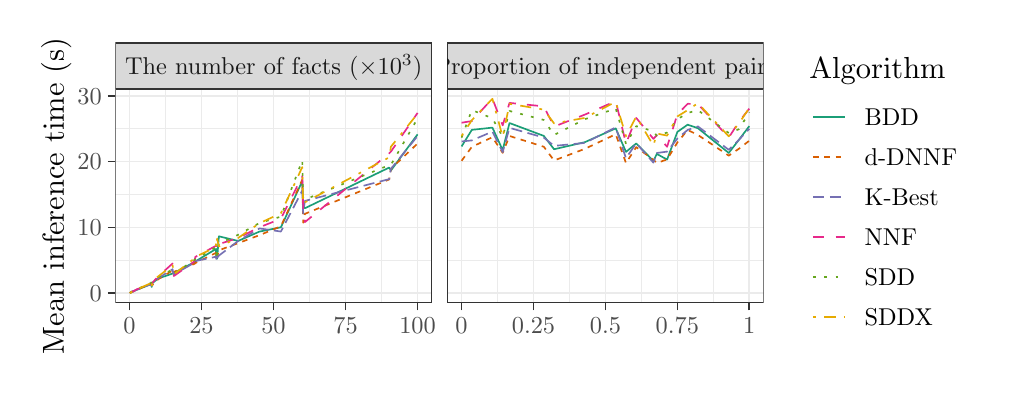
\begin{tikzpicture}[x=1pt,y=1pt]
\definecolor{fillColor}{RGB}{255,255,255}
\path[use as bounding box,fill=fillColor,fill opacity=0.00] (0,0) rectangle (346.90,130.09);
\begin{scope}
\path[clip] (  0.00,  0.00) rectangle (346.90,130.09);
\definecolor{drawColor}{RGB}{255,255,255}
\definecolor{fillColor}{RGB}{255,255,255}

\path[draw=drawColor,line width= 0.6pt,line join=round,line cap=round,fill=fillColor] (  0.00,  0.00) rectangle (346.90,130.09);
\end{scope}
\begin{scope}
\path[clip] ( 31.71, 30.69) rectangle (146.09,108.01);
\definecolor{fillColor}{RGB}{255,255,255}

\path[fill=fillColor] ( 31.71, 30.69) rectangle (146.09,108.01);
\definecolor{drawColor}{gray}{0.92}

\path[draw=drawColor,line width= 0.3pt,line join=round] ( 31.71, 46.03) --
	(146.09, 46.03);

\path[draw=drawColor,line width= 0.3pt,line join=round] ( 31.71, 69.81) --
	(146.09, 69.81);

\path[draw=drawColor,line width= 0.3pt,line join=round] ( 31.71, 93.59) --
	(146.09, 93.59);

\path[draw=drawColor,line width= 0.3pt,line join=round] ( 49.77, 30.69) --
	( 49.77,108.01);

\path[draw=drawColor,line width= 0.3pt,line join=round] ( 75.80, 30.69) --
	( 75.80,108.01);

\path[draw=drawColor,line width= 0.3pt,line join=round] (101.84, 30.69) --
	(101.84,108.01);

\path[draw=drawColor,line width= 0.3pt,line join=round] (127.87, 30.69) --
	(127.87,108.01);

\path[draw=drawColor,line width= 0.6pt,line join=round] ( 31.71, 34.14) --
	(146.09, 34.14);

\path[draw=drawColor,line width= 0.6pt,line join=round] ( 31.71, 57.92) --
	(146.09, 57.92);

\path[draw=drawColor,line width= 0.6pt,line join=round] ( 31.71, 81.70) --
	(146.09, 81.70);

\path[draw=drawColor,line width= 0.6pt,line join=round] ( 31.71,105.48) --
	(146.09,105.48);

\path[draw=drawColor,line width= 0.6pt,line join=round] ( 36.75, 30.69) --
	( 36.75,108.01);

\path[draw=drawColor,line width= 0.6pt,line join=round] ( 62.79, 30.69) --
	( 62.79,108.01);

\path[draw=drawColor,line width= 0.6pt,line join=round] ( 88.82, 30.69) --
	( 88.82,108.01);

\path[draw=drawColor,line width= 0.6pt,line join=round] (114.85, 30.69) --
	(114.85,108.01);

\path[draw=drawColor,line width= 0.6pt,line join=round] (140.89, 30.69) --
	(140.89,108.01);
\definecolor{drawColor}{RGB}{27,158,119}

\path[draw=drawColor,line width= 0.6pt,line join=round] ( 36.91, 34.22) --
	( 37.07, 34.28) --
	( 37.38, 34.45) --
	( 37.80, 34.74) --
	( 38.00, 34.74) --
	( 39.25, 35.27) --
	( 44.64, 37.45) --
	( 44.80, 36.38) --
	( 45.11, 37.84) --
	( 47.17, 39.46) --
	( 52.37, 41.24) --
	( 52.53, 41.31) --
	( 52.84, 41.51) --
	( 60.26, 45.33) --
	( 60.58, 45.62) --
	( 67.99, 50.08) --
	( 68.15, 47.64) --
	( 68.31, 50.15) --
	( 68.46, 46.59) --
	( 69.09, 54.70) --
	( 76.04, 53.02) --
	( 83.77, 56.41) --
	( 91.50, 57.95) --
	( 99.23, 74.63) --
	( 99.55, 65.78) --
	(100.17, 64.84) --
	(130.63, 79.54) --
	(131.26, 78.48) --
	(140.89, 91.54);
\definecolor{drawColor}{RGB}{217,95,2}

\path[draw=drawColor,line width= 0.6pt,dash pattern=on 2pt off 2pt ,line join=round] ( 36.91, 34.20) --
	( 37.07, 34.26) --
	( 37.38, 34.41) --
	( 37.80, 34.70) --
	( 38.00, 34.68) --
	( 39.25, 35.23) --
	( 44.64, 37.74) --
	( 44.80, 37.05) --
	( 45.11, 37.14) --
	( 47.17, 39.19) --
	( 52.37, 42.35) --
	( 52.53, 40.98) --
	( 52.84, 41.86) --
	( 60.26, 44.75) --
	( 60.58, 45.01) --
	( 67.99, 48.70) --
	( 68.15, 46.51) --
	( 68.31, 47.05) --
	( 68.46, 47.32) --
	( 69.09, 49.64) --
	( 76.04, 52.22) --
	( 83.77, 55.11) --
	( 91.50, 58.33) --
	( 99.23, 75.16) --
	( 99.55, 59.59) --
	(100.17, 62.82) --
	(130.63, 75.24) --
	(131.26, 79.11) --
	(140.89, 88.23);
\definecolor{drawColor}{RGB}{117,112,179}

\path[draw=drawColor,line width= 0.6pt,dash pattern=on 4pt off 2pt ,line join=round] ( 36.91, 34.22) --
	( 37.07, 34.33) --
	( 37.38, 34.49) --
	( 37.80, 34.77) --
	( 38.00, 34.77) --
	( 39.25, 35.37) --
	( 44.64, 37.40) --
	( 44.80, 36.84) --
	( 45.11, 37.68) --
	( 47.17, 39.58) --
	( 52.37, 42.81) --
	( 52.53, 41.77) --
	( 52.84, 40.98) --
	( 60.26, 45.16) --
	( 60.58, 45.74) --
	( 67.99, 47.31) --
	( 68.15, 46.52) --
	( 68.31, 48.59) --
	( 68.46, 46.96) --
	( 69.09, 47.72) --
	( 76.04, 52.99) --
	( 83.77, 57.55) --
	( 91.50, 56.42) --
	( 99.23, 71.23) --
	( 99.55, 62.93) --
	(100.17, 67.49) --
	(130.63, 75.36) --
	(131.26, 79.09) --
	(140.89, 90.92);
\definecolor{drawColor}{RGB}{231,41,138}

\path[draw=drawColor,line width= 0.6pt,dash pattern=on 4pt off 4pt ,line join=round] ( 36.91, 34.22) --
	( 37.07, 34.29) --
	( 37.38, 34.48) --
	( 37.80, 34.79) --
	( 38.00, 34.74) --
	( 39.25, 35.45) --
	( 44.64, 37.64) --
	( 44.80, 37.18) --
	( 45.11, 37.98) --
	( 47.17, 40.20) --
	( 52.37, 44.88) --
	( 52.53, 42.06) --
	( 52.84, 40.35) --
	( 60.26, 45.65) --
	( 60.58, 47.25) --
	( 67.99, 51.25) --
	( 68.15, 51.16) --
	( 68.31, 51.25) --
	( 68.46, 52.79) --
	( 69.09, 51.87) --
	( 76.04, 54.08) --
	( 83.77, 57.97) --
	( 91.50, 61.03) --
	( 99.23, 76.47) --
	( 99.55, 65.20) --
	(100.17, 59.83) --
	(130.63, 84.66) --
	(131.26, 85.31) --
	(140.89, 99.29);
\definecolor{drawColor}{RGB}{102,166,30}

\path[draw=drawColor,line width= 0.6pt,dash pattern=on 1pt off 3pt ,line join=round] ( 36.91, 34.24) --
	( 37.07, 34.31) --
	( 37.38, 34.48) --
	( 37.80, 34.81) --
	( 38.00, 34.77) --
	( 39.25, 35.45) --
	( 44.64, 37.88) --
	( 44.80, 38.54) --
	( 45.11, 38.69) --
	( 47.17, 39.95) --
	( 52.37, 42.70) --
	( 52.53, 41.93) --
	( 52.84, 41.20) --
	( 60.26, 46.14) --
	( 60.58, 46.43) --
	( 67.99, 50.70) --
	( 68.15, 47.87) --
	( 68.31, 50.28) --
	( 68.46, 47.98) --
	( 69.09, 52.07) --
	( 76.04, 55.24) --
	( 83.77, 59.51) --
	( 91.50, 61.81) --
	( 99.23, 82.15) --
	( 99.55, 68.77) --
	(100.17, 67.98) --
	(130.63, 80.43) --
	(131.26, 80.51) --
	(140.89, 97.30);
\definecolor{drawColor}{RGB}{230,171,2}

\path[draw=drawColor,line width= 0.6pt,dash pattern=on 1pt off 3pt on 4pt off 3pt ,line join=round] ( 36.91, 34.20) --
	( 37.07, 34.32) --
	( 37.38, 34.47) --
	( 37.80, 34.80) --
	( 38.00, 34.78) --
	( 39.25, 35.44) --
	( 44.64, 37.83) --
	( 44.80, 36.07) --
	( 45.11, 38.73) --
	( 47.17, 40.20) --
	( 52.37, 44.23) --
	( 52.53, 43.29) --
	( 52.84, 40.97) --
	( 60.26, 46.70) --
	( 60.58, 47.28) --
	( 67.99, 50.76) --
	( 68.15, 52.81) --
	( 68.31, 51.86) --
	( 68.46, 53.84) --
	( 69.09, 51.03) --
	( 76.04, 54.08) --
	( 83.77, 59.44) --
	( 91.50, 63.01) --
	( 99.23, 79.72) --
	( 99.55, 66.18) --
	(100.17, 66.97) --
	(130.63, 83.22) --
	(131.26, 87.08) --
	(140.89, 98.99);
\definecolor{drawColor}{gray}{0.20}

\path[draw=drawColor,line width= 0.6pt,line join=round,line cap=round] ( 31.71, 30.69) rectangle (146.09,108.01);
\end{scope}
\begin{scope}
\path[clip] (151.59, 30.69) rectangle (265.96,108.01);
\definecolor{fillColor}{RGB}{255,255,255}

\path[fill=fillColor] (151.59, 30.69) rectangle (265.96,108.01);
\definecolor{drawColor}{gray}{0.92}

\path[draw=drawColor,line width= 0.3pt,line join=round] (151.59, 46.03) --
	(265.96, 46.03);

\path[draw=drawColor,line width= 0.3pt,line join=round] (151.59, 69.81) --
	(265.96, 69.81);

\path[draw=drawColor,line width= 0.3pt,line join=round] (151.59, 93.59) --
	(265.96, 93.59);

\path[draw=drawColor,line width= 0.3pt,line join=round] (169.78, 30.69) --
	(169.78,108.01);

\path[draw=drawColor,line width= 0.3pt,line join=round] (195.78, 30.69) --
	(195.78,108.01);

\path[draw=drawColor,line width= 0.3pt,line join=round] (221.77, 30.69) --
	(221.77,108.01);

\path[draw=drawColor,line width= 0.3pt,line join=round] (247.77, 30.69) --
	(247.77,108.01);

\path[draw=drawColor,line width= 0.6pt,line join=round] (151.59, 34.14) --
	(265.96, 34.14);

\path[draw=drawColor,line width= 0.6pt,line join=round] (151.59, 57.92) --
	(265.96, 57.92);

\path[draw=drawColor,line width= 0.6pt,line join=round] (151.59, 81.70) --
	(265.96, 81.70);

\path[draw=drawColor,line width= 0.6pt,line join=round] (151.59,105.48) --
	(265.96,105.48);

\path[draw=drawColor,line width= 0.6pt,line join=round] (156.79, 30.69) --
	(156.79,108.01);

\path[draw=drawColor,line width= 0.6pt,line join=round] (182.78, 30.69) --
	(182.78,108.01);

\path[draw=drawColor,line width= 0.6pt,line join=round] (208.77, 30.69) --
	(208.77,108.01);

\path[draw=drawColor,line width= 0.6pt,line join=round] (234.77, 30.69) --
	(234.77,108.01);

\path[draw=drawColor,line width= 0.6pt,line join=round] (260.76, 30.69) --
	(260.76,108.01);
\definecolor{drawColor}{RGB}{27,158,119}

\path[draw=drawColor,line width= 0.6pt,line join=round] (156.79, 87.17) --
	(160.50, 93.17) --
	(167.93, 93.97) --
	(171.64, 85.86) --
	(174.11, 95.63) --
	(186.49, 90.99) --
	(190.21, 86.16) --
	(201.35, 88.72) --
	(212.49, 93.71) --
	(216.20, 85.21) --
	(219.91, 88.26) --
	(226.10, 81.94) --
	(227.34, 84.46) --
	(231.05, 82.43) --
	(234.77, 92.42) --
	(238.48, 95.04) --
	(242.19, 93.76) --
	(253.34, 84.82) --
	(257.05, 89.64) --
	(260.76, 94.51);
\definecolor{drawColor}{RGB}{217,95,2}

\path[draw=drawColor,line width= 0.6pt,dash pattern=on 2pt off 2pt ,line join=round] (156.79, 81.98) --
	(160.50, 87.03) --
	(167.93, 90.51) --
	(171.64, 84.86) --
	(174.11, 90.95) --
	(186.49, 87.07) --
	(190.21, 82.10) --
	(201.35, 86.31) --
	(212.49, 91.58) --
	(216.20, 81.17) --
	(219.91, 86.92) --
	(226.10, 82.36) --
	(227.34, 81.20) --
	(231.05, 82.46) --
	(234.77, 88.61) --
	(238.48, 93.14) --
	(242.19, 91.31) --
	(253.34, 83.85) --
	(257.05, 86.37) --
	(260.76, 89.25);
\definecolor{drawColor}{RGB}{117,112,179}

\path[draw=drawColor,line width= 0.6pt,dash pattern=on 4pt off 2pt ,line join=round] (156.79, 88.97) --
	(160.50, 89.35) --
	(167.93, 92.54) --
	(171.64, 85.10) --
	(174.11, 93.89) --
	(186.49, 90.38) --
	(190.21, 87.37) --
	(201.35, 88.45) --
	(212.49, 94.07) --
	(216.20, 82.90) --
	(219.91, 88.35) --
	(226.10, 81.32) --
	(227.34, 84.81) --
	(231.05, 85.30) --
	(234.77, 90.02) --
	(238.48, 93.14) --
	(242.19, 94.41) --
	(253.34, 85.94) --
	(257.05, 89.62) --
	(260.76, 93.56);
\definecolor{drawColor}{RGB}{231,41,138}

\path[draw=drawColor,line width= 0.6pt,dash pattern=on 4pt off 4pt ,line join=round] (156.79, 95.74) --
	(160.50, 96.35) --
	(167.93,104.50) --
	(171.64, 94.79) --
	(174.11,102.91) --
	(186.49,101.65) --
	(190.21, 94.35) --
	(201.35, 98.68) --
	(212.49,103.55) --
	(216.20, 88.20) --
	(219.91, 97.47) --
	(226.10, 89.92) --
	(227.34, 91.22) --
	(231.05, 87.06) --
	(234.77, 98.75) --
	(238.48,102.58) --
	(242.19,102.50) --
	(253.34, 90.37) --
	(257.05, 96.15) --
	(260.76,100.82);
\definecolor{drawColor}{RGB}{102,166,30}

\path[draw=drawColor,line width= 0.6pt,dash pattern=on 1pt off 3pt ,line join=round] (156.79, 90.34) --
	(160.50,100.33) --
	(167.93, 97.34) --
	(171.64, 90.63) --
	(174.11, 99.99) --
	(186.49, 96.75) --
	(190.21, 91.32) --
	(201.35, 97.00) --
	(212.49,100.90) --
	(216.20, 88.11) --
	(219.91, 94.51) --
	(226.10, 92.66) --
	(227.34, 90.99) --
	(231.05, 92.19) --
	(234.77, 96.98) --
	(238.48, 99.26) --
	(242.19,100.29) --
	(253.34, 92.01) --
	(257.05, 93.41) --
	(260.76, 99.52);
\definecolor{drawColor}{RGB}{230,171,2}

\path[draw=drawColor,line width= 0.6pt,dash pattern=on 1pt off 3pt on 4pt off 3pt ,line join=round] (156.79, 90.96) --
	(160.50, 96.67) --
	(167.93,104.39) --
	(171.64, 90.59) --
	(174.11,102.58) --
	(186.49,100.48) --
	(190.21, 95.50) --
	(201.35, 97.48) --
	(212.49,103.31) --
	(216.20, 90.87) --
	(219.91, 97.96) --
	(226.10, 87.48) --
	(227.34, 91.85) --
	(231.05, 91.08) --
	(234.77, 98.02) --
	(238.48,100.29) --
	(242.19,102.81) --
	(253.34, 90.81) --
	(257.05, 95.58) --
	(260.76,101.07);
\definecolor{drawColor}{gray}{0.20}

\path[draw=drawColor,line width= 0.6pt,line join=round,line cap=round] (151.59, 30.69) rectangle (265.96,108.01);
\end{scope}
\begin{scope}
\path[clip] ( 31.71,108.01) rectangle (146.09,124.59);
\definecolor{drawColor}{gray}{0.20}
\definecolor{fillColor}{gray}{0.85}

\path[draw=drawColor,line width= 0.6pt,line join=round,line cap=round,fill=fillColor] ( 31.71,108.01) rectangle (146.09,124.59);
\definecolor{drawColor}{gray}{0.10}

\node[text=drawColor,anchor=base,inner sep=0pt, outer sep=0pt, scale=  0.88] at ( 88.90,113.27) {The number of facts ($\times 10^3$)};
\end{scope}
\begin{scope}
\path[clip] (151.59,108.01) rectangle (265.96,124.59);
\definecolor{drawColor}{gray}{0.20}
\definecolor{fillColor}{gray}{0.85}

\path[draw=drawColor,line width= 0.6pt,line join=round,line cap=round,fill=fillColor] (151.59,108.01) rectangle (265.96,124.59);
\definecolor{drawColor}{gray}{0.10}

\node[text=drawColor,anchor=base,inner sep=0pt, outer sep=0pt, scale=  0.88] at (208.77,113.27) {Proportion of independent pairs};
\end{scope}
\begin{scope}
\path[clip] (  0.00,  0.00) rectangle (346.90,130.09);
\definecolor{drawColor}{gray}{0.20}

\path[draw=drawColor,line width= 0.6pt,line join=round] ( 36.75, 27.94) --
	( 36.75, 30.69);

\path[draw=drawColor,line width= 0.6pt,line join=round] ( 62.79, 27.94) --
	( 62.79, 30.69);

\path[draw=drawColor,line width= 0.6pt,line join=round] ( 88.82, 27.94) --
	( 88.82, 30.69);

\path[draw=drawColor,line width= 0.6pt,line join=round] (114.85, 27.94) --
	(114.85, 30.69);

\path[draw=drawColor,line width= 0.6pt,line join=round] (140.89, 27.94) --
	(140.89, 30.69);
\end{scope}
\begin{scope}
\path[clip] (  0.00,  0.00) rectangle (346.90,130.09);
\definecolor{drawColor}{gray}{0.30}

\node[text=drawColor,anchor=base,inner sep=0pt, outer sep=0pt, scale=  0.88] at ( 36.75, 19.68) {0};

\node[text=drawColor,anchor=base,inner sep=0pt, outer sep=0pt, scale=  0.88] at ( 62.79, 19.68) {25};

\node[text=drawColor,anchor=base,inner sep=0pt, outer sep=0pt, scale=  0.88] at ( 88.82, 19.68) {50};

\node[text=drawColor,anchor=base,inner sep=0pt, outer sep=0pt, scale=  0.88] at (114.85, 19.68) {75};

\node[text=drawColor,anchor=base,inner sep=0pt, outer sep=0pt, scale=  0.88] at (140.89, 19.68) {100};
\end{scope}
\begin{scope}
\path[clip] (  0.00,  0.00) rectangle (346.90,130.09);
\definecolor{drawColor}{gray}{0.20}

\path[draw=drawColor,line width= 0.6pt,line join=round] (156.79, 27.94) --
	(156.79, 30.69);

\path[draw=drawColor,line width= 0.6pt,line join=round] (182.78, 27.94) --
	(182.78, 30.69);

\path[draw=drawColor,line width= 0.6pt,line join=round] (208.77, 27.94) --
	(208.77, 30.69);

\path[draw=drawColor,line width= 0.6pt,line join=round] (234.77, 27.94) --
	(234.77, 30.69);

\path[draw=drawColor,line width= 0.6pt,line join=round] (260.76, 27.94) --
	(260.76, 30.69);
\end{scope}
\begin{scope}
\path[clip] (  0.00,  0.00) rectangle (346.90,130.09);
\definecolor{drawColor}{gray}{0.30}

\node[text=drawColor,anchor=base,inner sep=0pt, outer sep=0pt, scale=  0.88] at (156.79, 19.68) {0};

\node[text=drawColor,anchor=base,inner sep=0pt, outer sep=0pt, scale=  0.88] at (182.78, 19.68) {0.25};

\node[text=drawColor,anchor=base,inner sep=0pt, outer sep=0pt, scale=  0.88] at (208.77, 19.68) {0.5};

\node[text=drawColor,anchor=base,inner sep=0pt, outer sep=0pt, scale=  0.88] at (234.77, 19.68) {0.75};

\node[text=drawColor,anchor=base,inner sep=0pt, outer sep=0pt, scale=  0.88] at (260.76, 19.68) {1};
\end{scope}
\begin{scope}
\path[clip] (  0.00,  0.00) rectangle (346.90,130.09);
\definecolor{drawColor}{gray}{0.30}

\node[text=drawColor,anchor=base east,inner sep=0pt, outer sep=0pt, scale=  0.88] at ( 26.76, 31.11) {0};

\node[text=drawColor,anchor=base east,inner sep=0pt, outer sep=0pt, scale=  0.88] at ( 26.76, 54.89) {10};

\node[text=drawColor,anchor=base east,inner sep=0pt, outer sep=0pt, scale=  0.88] at ( 26.76, 78.67) {20};

\node[text=drawColor,anchor=base east,inner sep=0pt, outer sep=0pt, scale=  0.88] at ( 26.76,102.45) {30};
\end{scope}
\begin{scope}
\path[clip] (  0.00,  0.00) rectangle (346.90,130.09);
\definecolor{drawColor}{gray}{0.20}

\path[draw=drawColor,line width= 0.6pt,line join=round] ( 28.96, 34.14) --
	( 31.71, 34.14);

\path[draw=drawColor,line width= 0.6pt,line join=round] ( 28.96, 57.92) --
	( 31.71, 57.92);

\path[draw=drawColor,line width= 0.6pt,line join=round] ( 28.96, 81.70) --
	( 31.71, 81.70);

\path[draw=drawColor,line width= 0.6pt,line join=round] ( 28.96,105.48) --
	( 31.71,105.48);
\end{scope}
\begin{scope}
\path[clip] (  0.00,  0.00) rectangle (346.90,130.09);
\definecolor{drawColor}{RGB}{0,0,0}

\node[text=drawColor,rotate= 90.00,anchor=base,inner sep=0pt, outer sep=0pt, scale=  1.10] at ( 13.08, 69.35) {Mean inference time (s)};
\end{scope}
\begin{scope}
\path[clip] (  0.00,  0.00) rectangle (346.90,130.09);
\definecolor{fillColor}{RGB}{255,255,255}

\path[fill=fillColor] (276.96, 12.88) rectangle (341.40,125.82);
\end{scope}
\begin{scope}
\path[clip] (  0.00,  0.00) rectangle (346.90,130.09);
\definecolor{drawColor}{RGB}{0,0,0}

\node[text=drawColor,anchor=base west,inner sep=0pt, outer sep=0pt, scale=  1.10] at (282.46,111.67) {Algorithm};
\end{scope}
\begin{scope}
\path[clip] (  0.00,  0.00) rectangle (346.90,130.09);
\definecolor{fillColor}{RGB}{255,255,255}

\path[fill=fillColor] (282.46, 90.65) rectangle (296.92,105.10);
\end{scope}
\begin{scope}
\path[clip] (  0.00,  0.00) rectangle (346.90,130.09);
\definecolor{drawColor}{RGB}{27,158,119}

\path[draw=drawColor,line width= 0.6pt,line join=round] (283.91, 97.88) -- (295.47, 97.88);
\end{scope}
\begin{scope}
\path[clip] (  0.00,  0.00) rectangle (346.90,130.09);
\definecolor{fillColor}{RGB}{255,255,255}

\path[fill=fillColor] (282.46, 76.20) rectangle (296.92, 90.65);
\end{scope}
\begin{scope}
\path[clip] (  0.00,  0.00) rectangle (346.90,130.09);
\definecolor{drawColor}{RGB}{217,95,2}

\path[draw=drawColor,line width= 0.6pt,dash pattern=on 2pt off 2pt ,line join=round] (283.91, 83.42) -- (295.47, 83.42);
\end{scope}
\begin{scope}
\path[clip] (  0.00,  0.00) rectangle (346.90,130.09);
\definecolor{fillColor}{RGB}{255,255,255}

\path[fill=fillColor] (282.46, 61.74) rectangle (296.92, 76.20);
\end{scope}
\begin{scope}
\path[clip] (  0.00,  0.00) rectangle (346.90,130.09);
\definecolor{drawColor}{RGB}{117,112,179}

\path[draw=drawColor,line width= 0.6pt,dash pattern=on 4pt off 2pt ,line join=round] (283.91, 68.97) -- (295.47, 68.97);
\end{scope}
\begin{scope}
\path[clip] (  0.00,  0.00) rectangle (346.90,130.09);
\definecolor{fillColor}{RGB}{255,255,255}

\path[fill=fillColor] (282.46, 47.29) rectangle (296.92, 61.74);
\end{scope}
\begin{scope}
\path[clip] (  0.00,  0.00) rectangle (346.90,130.09);
\definecolor{drawColor}{RGB}{231,41,138}

\path[draw=drawColor,line width= 0.6pt,dash pattern=on 4pt off 4pt ,line join=round] (283.91, 54.52) -- (295.47, 54.52);
\end{scope}
\begin{scope}
\path[clip] (  0.00,  0.00) rectangle (346.90,130.09);
\definecolor{fillColor}{RGB}{255,255,255}

\path[fill=fillColor] (282.46, 32.83) rectangle (296.92, 47.29);
\end{scope}
\begin{scope}
\path[clip] (  0.00,  0.00) rectangle (346.90,130.09);
\definecolor{drawColor}{RGB}{102,166,30}

\path[draw=drawColor,line width= 0.6pt,dash pattern=on 1pt off 3pt ,line join=round] (283.91, 40.06) -- (295.47, 40.06);
\end{scope}
\begin{scope}
\path[clip] (  0.00,  0.00) rectangle (346.90,130.09);
\definecolor{fillColor}{RGB}{255,255,255}

\path[fill=fillColor] (282.46, 18.38) rectangle (296.92, 32.83);
\end{scope}
\begin{scope}
\path[clip] (  0.00,  0.00) rectangle (346.90,130.09);
\definecolor{drawColor}{RGB}{230,171,2}

\path[draw=drawColor,line width= 0.6pt,dash pattern=on 1pt off 3pt on 4pt off 3pt ,line join=round] (283.91, 25.61) -- (295.47, 25.61);
\end{scope}
\begin{scope}
\path[clip] (  0.00,  0.00) rectangle (346.90,130.09);
\definecolor{drawColor}{RGB}{0,0,0}

\node[text=drawColor,anchor=base west,inner sep=0pt, outer sep=0pt, scale=  0.88] at (302.42, 94.85) {BDD};
\end{scope}
\begin{scope}
\path[clip] (  0.00,  0.00) rectangle (346.90,130.09);
\definecolor{drawColor}{RGB}{0,0,0}

\node[text=drawColor,anchor=base west,inner sep=0pt, outer sep=0pt, scale=  0.88] at (302.42, 80.39) {d-DNNF};
\end{scope}
\begin{scope}
\path[clip] (  0.00,  0.00) rectangle (346.90,130.09);
\definecolor{drawColor}{RGB}{0,0,0}

\node[text=drawColor,anchor=base west,inner sep=0pt, outer sep=0pt, scale=  0.88] at (302.42, 65.94) {K-Best};
\end{scope}
\begin{scope}
\path[clip] (  0.00,  0.00) rectangle (346.90,130.09);
\definecolor{drawColor}{RGB}{0,0,0}

\node[text=drawColor,anchor=base west,inner sep=0pt, outer sep=0pt, scale=  0.88] at (302.42, 51.49) {NNF};
\end{scope}
\begin{scope}
\path[clip] (  0.00,  0.00) rectangle (346.90,130.09);
\definecolor{drawColor}{RGB}{0,0,0}

\node[text=drawColor,anchor=base west,inner sep=0pt, outer sep=0pt, scale=  0.88] at (302.42, 37.03) {SDD};
\end{scope}
\begin{scope}
\path[clip] (  0.00,  0.00) rectangle (346.90,130.09);
\definecolor{drawColor}{RGB}{0,0,0}

\node[text=drawColor,anchor=base west,inner sep=0pt, outer sep=0pt, scale=  0.88] at (302.42, 22.58) {SDDX};
\end{scope}
\end{tikzpicture}
}
  \end{figure}
\end{frame}

\begin{frame}{How Program Features Influence Inference Time}
  \begin{figure}
    \centering
    % Created by tikzDevice version 0.12.3 on 2020-05-14 17:55:45
% !TEX encoding = UTF-8 Unicode
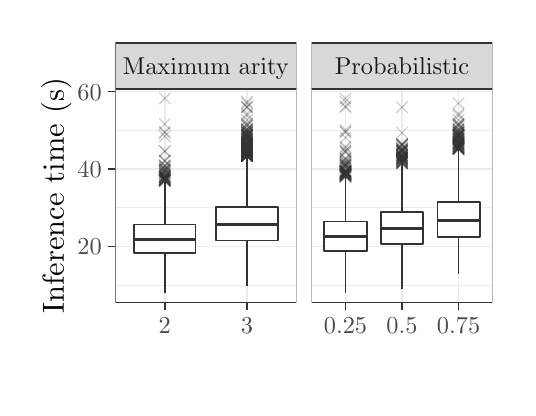
\begin{tikzpicture}[x=1pt,y=1pt]
\definecolor{fillColor}{RGB}{255,255,255}
\path[use as bounding box,fill=fillColor,fill opacity=0.00] (0,0) rectangle (173.45,130.09);
\begin{scope}
\path[clip] (  0.00,  0.00) rectangle (173.45,130.09);
\definecolor{drawColor}{RGB}{255,255,255}
\definecolor{fillColor}{RGB}{255,255,255}

\path[draw=drawColor,line width= 0.6pt,line join=round,line cap=round,fill=fillColor] ( -0.00,  0.00) rectangle (173.45,130.09);
\end{scope}
\begin{scope}
\path[clip] ( 31.71, 30.69) rectangle ( 97.08,108.01);
\definecolor{fillColor}{RGB}{255,255,255}

\path[fill=fillColor] ( 31.71, 30.69) rectangle ( 97.08,108.01);
\definecolor{drawColor}{gray}{0.92}

\path[draw=drawColor,line width= 0.3pt,line join=round] ( 31.71, 36.97) --
	( 97.08, 36.97);

\path[draw=drawColor,line width= 0.3pt,line join=round] ( 31.71, 64.98) --
	( 97.08, 64.98);

\path[draw=drawColor,line width= 0.3pt,line join=round] ( 31.71, 92.98) --
	( 97.08, 92.98);

\path[draw=drawColor,line width= 0.6pt,line join=round] ( 31.71, 50.98) --
	( 97.08, 50.98);

\path[draw=drawColor,line width= 0.6pt,line join=round] ( 31.71, 78.98) --
	( 97.08, 78.98);

\path[draw=drawColor,line width= 0.6pt,line join=round] ( 31.71,106.99) --
	( 97.08,106.99);

\path[draw=drawColor,line width= 0.6pt,line join=round] ( 49.54, 30.69) --
	( 49.54,108.01);

\path[draw=drawColor,line width= 0.6pt,line join=round] ( 79.25, 30.69) --
	( 79.25,108.01);
\definecolor{drawColor}{RGB}{51,51,51}

\path[draw=drawColor,draw opacity=0.25,line width= 0.4pt,line join=round,line cap=round] ( 47.58, 74.50) -- ( 51.50, 78.42);

\path[draw=drawColor,draw opacity=0.25,line width= 0.4pt,line join=round,line cap=round] ( 47.58, 78.42) -- ( 51.50, 74.50);

\path[draw=drawColor,draw opacity=0.25,line width= 0.4pt,line join=round,line cap=round] ( 47.58, 73.55) -- ( 51.50, 77.47);

\path[draw=drawColor,draw opacity=0.25,line width= 0.4pt,line join=round,line cap=round] ( 47.58, 77.47) -- ( 51.50, 73.55);

\path[draw=drawColor,draw opacity=0.25,line width= 0.4pt,line join=round,line cap=round] ( 47.58, 83.41) -- ( 51.50, 87.33);

\path[draw=drawColor,draw opacity=0.25,line width= 0.4pt,line join=round,line cap=round] ( 47.58, 87.33) -- ( 51.50, 83.41);

\path[draw=drawColor,draw opacity=0.25,line width= 0.4pt,line join=round,line cap=round] ( 47.58, 78.42) -- ( 51.50, 82.34);

\path[draw=drawColor,draw opacity=0.25,line width= 0.4pt,line join=round,line cap=round] ( 47.58, 82.34) -- ( 51.50, 78.42);

\path[draw=drawColor,draw opacity=0.25,line width= 0.4pt,line join=round,line cap=round] ( 47.58, 76.11) -- ( 51.50, 80.03);

\path[draw=drawColor,draw opacity=0.25,line width= 0.4pt,line join=round,line cap=round] ( 47.58, 80.03) -- ( 51.50, 76.11);

\path[draw=drawColor,draw opacity=0.25,line width= 0.4pt,line join=round,line cap=round] ( 47.58, 74.48) -- ( 51.50, 78.40);

\path[draw=drawColor,draw opacity=0.25,line width= 0.4pt,line join=round,line cap=round] ( 47.58, 78.40) -- ( 51.50, 74.48);

\path[draw=drawColor,draw opacity=0.25,line width= 0.4pt,line join=round,line cap=round] ( 47.58, 76.90) -- ( 51.50, 80.82);

\path[draw=drawColor,draw opacity=0.25,line width= 0.4pt,line join=round,line cap=round] ( 47.58, 80.82) -- ( 51.50, 76.90);

\path[draw=drawColor,draw opacity=0.25,line width= 0.4pt,line join=round,line cap=round] ( 47.58, 72.95) -- ( 51.50, 76.87);

\path[draw=drawColor,draw opacity=0.25,line width= 0.4pt,line join=round,line cap=round] ( 47.58, 76.87) -- ( 51.50, 72.95);

\path[draw=drawColor,draw opacity=0.25,line width= 0.4pt,line join=round,line cap=round] ( 47.58, 77.09) -- ( 51.50, 81.02);

\path[draw=drawColor,draw opacity=0.25,line width= 0.4pt,line join=round,line cap=round] ( 47.58, 81.02) -- ( 51.50, 77.09);

\path[draw=drawColor,draw opacity=0.25,line width= 0.4pt,line join=round,line cap=round] ( 47.58, 74.11) -- ( 51.50, 78.03);

\path[draw=drawColor,draw opacity=0.25,line width= 0.4pt,line join=round,line cap=round] ( 47.58, 78.03) -- ( 51.50, 74.11);

\path[draw=drawColor,draw opacity=0.25,line width= 0.4pt,line join=round,line cap=round] ( 47.58, 76.69) -- ( 51.50, 80.62);

\path[draw=drawColor,draw opacity=0.25,line width= 0.4pt,line join=round,line cap=round] ( 47.58, 80.62) -- ( 51.50, 76.69);

\path[draw=drawColor,draw opacity=0.25,line width= 0.4pt,line join=round,line cap=round] ( 47.58, 75.42) -- ( 51.50, 79.34);

\path[draw=drawColor,draw opacity=0.25,line width= 0.4pt,line join=round,line cap=round] ( 47.58, 79.34) -- ( 51.50, 75.42);

\path[draw=drawColor,draw opacity=0.25,line width= 0.4pt,line join=round,line cap=round] ( 47.58, 73.74) -- ( 51.50, 77.67);

\path[draw=drawColor,draw opacity=0.25,line width= 0.4pt,line join=round,line cap=round] ( 47.58, 77.67) -- ( 51.50, 73.74);

\path[draw=drawColor,draw opacity=0.25,line width= 0.4pt,line join=round,line cap=round] ( 47.58, 74.11) -- ( 51.50, 78.03);

\path[draw=drawColor,draw opacity=0.25,line width= 0.4pt,line join=round,line cap=round] ( 47.58, 78.03) -- ( 51.50, 74.11);

\path[draw=drawColor,draw opacity=0.25,line width= 0.4pt,line join=round,line cap=round] ( 47.58, 74.03) -- ( 51.50, 77.96);

\path[draw=drawColor,draw opacity=0.25,line width= 0.4pt,line join=round,line cap=round] ( 47.58, 77.96) -- ( 51.50, 74.03);

\path[draw=drawColor,draw opacity=0.25,line width= 0.4pt,line join=round,line cap=round] ( 47.58, 76.80) -- ( 51.50, 80.72);

\path[draw=drawColor,draw opacity=0.25,line width= 0.4pt,line join=round,line cap=round] ( 47.58, 80.72) -- ( 51.50, 76.80);

\path[draw=drawColor,draw opacity=0.25,line width= 0.4pt,line join=round,line cap=round] ( 47.58, 74.58) -- ( 51.50, 78.50);

\path[draw=drawColor,draw opacity=0.25,line width= 0.4pt,line join=round,line cap=round] ( 47.58, 78.50) -- ( 51.50, 74.58);

\path[draw=drawColor,draw opacity=0.25,line width= 0.4pt,line join=round,line cap=round] ( 47.58, 73.04) -- ( 51.50, 76.96);

\path[draw=drawColor,draw opacity=0.25,line width= 0.4pt,line join=round,line cap=round] ( 47.58, 76.96) -- ( 51.50, 73.04);

\path[draw=drawColor,draw opacity=0.25,line width= 0.4pt,line join=round,line cap=round] ( 47.58, 74.11) -- ( 51.50, 78.03);

\path[draw=drawColor,draw opacity=0.25,line width= 0.4pt,line join=round,line cap=round] ( 47.58, 78.03) -- ( 51.50, 74.11);

\path[draw=drawColor,draw opacity=0.25,line width= 0.4pt,line join=round,line cap=round] ( 47.58, 74.24) -- ( 51.50, 78.16);

\path[draw=drawColor,draw opacity=0.25,line width= 0.4pt,line join=round,line cap=round] ( 47.58, 78.16) -- ( 51.50, 74.24);

\path[draw=drawColor,draw opacity=0.25,line width= 0.4pt,line join=round,line cap=round] ( 47.58, 73.75) -- ( 51.50, 77.68);

\path[draw=drawColor,draw opacity=0.25,line width= 0.4pt,line join=round,line cap=round] ( 47.58, 77.68) -- ( 51.50, 73.75);

\path[draw=drawColor,draw opacity=0.25,line width= 0.4pt,line join=round,line cap=round] ( 47.58, 73.33) -- ( 51.50, 77.25);

\path[draw=drawColor,draw opacity=0.25,line width= 0.4pt,line join=round,line cap=round] ( 47.58, 77.25) -- ( 51.50, 73.33);

\path[draw=drawColor,draw opacity=0.25,line width= 0.4pt,line join=round,line cap=round] ( 47.58, 75.34) -- ( 51.50, 79.26);

\path[draw=drawColor,draw opacity=0.25,line width= 0.4pt,line join=round,line cap=round] ( 47.58, 79.26) -- ( 51.50, 75.34);

\path[draw=drawColor,draw opacity=0.25,line width= 0.4pt,line join=round,line cap=round] ( 47.58, 75.66) -- ( 51.50, 79.58);

\path[draw=drawColor,draw opacity=0.25,line width= 0.4pt,line join=round,line cap=round] ( 47.58, 79.58) -- ( 51.50, 75.66);

\path[draw=drawColor,draw opacity=0.25,line width= 0.4pt,line join=round,line cap=round] ( 47.58, 72.71) -- ( 51.50, 76.63);

\path[draw=drawColor,draw opacity=0.25,line width= 0.4pt,line join=round,line cap=round] ( 47.58, 76.63) -- ( 51.50, 72.71);

\path[draw=drawColor,draw opacity=0.25,line width= 0.4pt,line join=round,line cap=round] ( 47.58, 77.76) -- ( 51.50, 81.69);

\path[draw=drawColor,draw opacity=0.25,line width= 0.4pt,line join=round,line cap=round] ( 47.58, 81.69) -- ( 51.50, 77.76);

\path[draw=drawColor,draw opacity=0.25,line width= 0.4pt,line join=round,line cap=round] ( 47.58, 76.89) -- ( 51.50, 80.82);

\path[draw=drawColor,draw opacity=0.25,line width= 0.4pt,line join=round,line cap=round] ( 47.58, 80.82) -- ( 51.50, 76.89);

\path[draw=drawColor,draw opacity=0.25,line width= 0.4pt,line join=round,line cap=round] ( 47.58, 74.43) -- ( 51.50, 78.36);

\path[draw=drawColor,draw opacity=0.25,line width= 0.4pt,line join=round,line cap=round] ( 47.58, 78.36) -- ( 51.50, 74.43);

\path[draw=drawColor,draw opacity=0.25,line width= 0.4pt,line join=round,line cap=round] ( 47.58, 73.36) -- ( 51.50, 77.29);

\path[draw=drawColor,draw opacity=0.25,line width= 0.4pt,line join=round,line cap=round] ( 47.58, 77.29) -- ( 51.50, 73.36);

\path[draw=drawColor,draw opacity=0.25,line width= 0.4pt,line join=round,line cap=round] ( 47.58, 73.28) -- ( 51.50, 77.20);

\path[draw=drawColor,draw opacity=0.25,line width= 0.4pt,line join=round,line cap=round] ( 47.58, 77.20) -- ( 51.50, 73.28);

\path[draw=drawColor,draw opacity=0.25,line width= 0.4pt,line join=round,line cap=round] ( 47.58, 73.81) -- ( 51.50, 77.73);

\path[draw=drawColor,draw opacity=0.25,line width= 0.4pt,line join=round,line cap=round] ( 47.58, 77.73) -- ( 51.50, 73.81);

\path[draw=drawColor,draw opacity=0.25,line width= 0.4pt,line join=round,line cap=round] ( 47.58, 76.10) -- ( 51.50, 80.03);

\path[draw=drawColor,draw opacity=0.25,line width= 0.4pt,line join=round,line cap=round] ( 47.58, 80.03) -- ( 51.50, 76.10);

\path[draw=drawColor,draw opacity=0.25,line width= 0.4pt,line join=round,line cap=round] ( 47.58, 75.24) -- ( 51.50, 79.16);

\path[draw=drawColor,draw opacity=0.25,line width= 0.4pt,line join=round,line cap=round] ( 47.58, 79.16) -- ( 51.50, 75.24);

\path[draw=drawColor,draw opacity=0.25,line width= 0.4pt,line join=round,line cap=round] ( 47.58, 78.38) -- ( 51.50, 82.31);

\path[draw=drawColor,draw opacity=0.25,line width= 0.4pt,line join=round,line cap=round] ( 47.58, 82.31) -- ( 51.50, 78.38);

\path[draw=drawColor,draw opacity=0.25,line width= 0.4pt,line join=round,line cap=round] ( 47.58, 72.51) -- ( 51.50, 76.43);

\path[draw=drawColor,draw opacity=0.25,line width= 0.4pt,line join=round,line cap=round] ( 47.58, 76.43) -- ( 51.50, 72.51);

\path[draw=drawColor,draw opacity=0.25,line width= 0.4pt,line join=round,line cap=round] ( 47.58, 74.85) -- ( 51.50, 78.78);

\path[draw=drawColor,draw opacity=0.25,line width= 0.4pt,line join=round,line cap=round] ( 47.58, 78.78) -- ( 51.50, 74.85);

\path[draw=drawColor,draw opacity=0.25,line width= 0.4pt,line join=round,line cap=round] ( 47.58, 72.89) -- ( 51.50, 76.82);

\path[draw=drawColor,draw opacity=0.25,line width= 0.4pt,line join=round,line cap=round] ( 47.58, 76.82) -- ( 51.50, 72.89);

\path[draw=drawColor,draw opacity=0.25,line width= 0.4pt,line join=round,line cap=round] ( 47.58, 73.54) -- ( 51.50, 77.46);

\path[draw=drawColor,draw opacity=0.25,line width= 0.4pt,line join=round,line cap=round] ( 47.58, 77.46) -- ( 51.50, 73.54);

\path[draw=drawColor,draw opacity=0.25,line width= 0.4pt,line join=round,line cap=round] ( 47.58, 79.88) -- ( 51.50, 83.81);

\path[draw=drawColor,draw opacity=0.25,line width= 0.4pt,line join=round,line cap=round] ( 47.58, 83.81) -- ( 51.50, 79.88);

\path[draw=drawColor,draw opacity=0.25,line width= 0.4pt,line join=round,line cap=round] ( 47.58,102.54) -- ( 51.50,106.46);

\path[draw=drawColor,draw opacity=0.25,line width= 0.4pt,line join=round,line cap=round] ( 47.58,106.46) -- ( 51.50,102.54);

\path[draw=drawColor,draw opacity=0.25,line width= 0.4pt,line join=round,line cap=round] ( 47.58, 88.89) -- ( 51.50, 92.81);

\path[draw=drawColor,draw opacity=0.25,line width= 0.4pt,line join=round,line cap=round] ( 47.58, 92.81) -- ( 51.50, 88.89);

\path[draw=drawColor,draw opacity=0.25,line width= 0.4pt,line join=round,line cap=round] ( 47.58, 73.05) -- ( 51.50, 76.97);

\path[draw=drawColor,draw opacity=0.25,line width= 0.4pt,line join=round,line cap=round] ( 47.58, 76.97) -- ( 51.50, 73.05);

\path[draw=drawColor,draw opacity=0.25,line width= 0.4pt,line join=round,line cap=round] ( 47.58, 73.11) -- ( 51.50, 77.03);

\path[draw=drawColor,draw opacity=0.25,line width= 0.4pt,line join=round,line cap=round] ( 47.58, 77.03) -- ( 51.50, 73.11);

\path[draw=drawColor,draw opacity=0.25,line width= 0.4pt,line join=round,line cap=round] ( 47.58, 73.17) -- ( 51.50, 77.09);

\path[draw=drawColor,draw opacity=0.25,line width= 0.4pt,line join=round,line cap=round] ( 47.58, 77.09) -- ( 51.50, 73.17);

\path[draw=drawColor,draw opacity=0.25,line width= 0.4pt,line join=round,line cap=round] ( 47.58, 72.85) -- ( 51.50, 76.77);

\path[draw=drawColor,draw opacity=0.25,line width= 0.4pt,line join=round,line cap=round] ( 47.58, 76.77) -- ( 51.50, 72.85);

\path[draw=drawColor,draw opacity=0.25,line width= 0.4pt,line join=round,line cap=round] ( 47.58, 80.27) -- ( 51.50, 84.20);

\path[draw=drawColor,draw opacity=0.25,line width= 0.4pt,line join=round,line cap=round] ( 47.58, 84.20) -- ( 51.50, 80.27);

\path[draw=drawColor,draw opacity=0.25,line width= 0.4pt,line join=round,line cap=round] ( 47.58, 83.55) -- ( 51.50, 87.47);

\path[draw=drawColor,draw opacity=0.25,line width= 0.4pt,line join=round,line cap=round] ( 47.58, 87.47) -- ( 51.50, 83.55);

\path[draw=drawColor,draw opacity=0.25,line width= 0.4pt,line join=round,line cap=round] ( 47.58, 90.50) -- ( 51.50, 94.42);

\path[draw=drawColor,draw opacity=0.25,line width= 0.4pt,line join=round,line cap=round] ( 47.58, 94.42) -- ( 51.50, 90.50);

\path[draw=drawColor,draw opacity=0.25,line width= 0.4pt,line join=round,line cap=round] ( 47.58, 76.52) -- ( 51.50, 80.45);

\path[draw=drawColor,draw opacity=0.25,line width= 0.4pt,line join=round,line cap=round] ( 47.58, 80.45) -- ( 51.50, 76.52);

\path[draw=drawColor,draw opacity=0.25,line width= 0.4pt,line join=round,line cap=round] ( 47.58, 75.93) -- ( 51.50, 79.85);

\path[draw=drawColor,draw opacity=0.25,line width= 0.4pt,line join=round,line cap=round] ( 47.58, 79.85) -- ( 51.50, 75.93);

\path[draw=drawColor,draw opacity=0.25,line width= 0.4pt,line join=round,line cap=round] ( 47.58, 73.09) -- ( 51.50, 77.02);

\path[draw=drawColor,draw opacity=0.25,line width= 0.4pt,line join=round,line cap=round] ( 47.58, 77.02) -- ( 51.50, 73.09);

\path[draw=drawColor,draw opacity=0.25,line width= 0.4pt,line join=round,line cap=round] ( 47.58, 73.21) -- ( 51.50, 77.13);

\path[draw=drawColor,draw opacity=0.25,line width= 0.4pt,line join=round,line cap=round] ( 47.58, 77.13) -- ( 51.50, 73.21);

\path[draw=drawColor,draw opacity=0.25,line width= 0.4pt,line join=round,line cap=round] ( 47.58, 77.77) -- ( 51.50, 81.69);

\path[draw=drawColor,draw opacity=0.25,line width= 0.4pt,line join=round,line cap=round] ( 47.58, 81.69) -- ( 51.50, 77.77);

\path[draw=drawColor,draw opacity=0.25,line width= 0.4pt,line join=round,line cap=round] ( 47.58, 73.08) -- ( 51.50, 77.01);

\path[draw=drawColor,draw opacity=0.25,line width= 0.4pt,line join=round,line cap=round] ( 47.58, 77.01) -- ( 51.50, 73.08);

\path[draw=drawColor,draw opacity=0.25,line width= 0.4pt,line join=round,line cap=round] ( 47.58, 90.09) -- ( 51.50, 94.01);

\path[draw=drawColor,draw opacity=0.25,line width= 0.4pt,line join=round,line cap=round] ( 47.58, 94.01) -- ( 51.50, 90.09);

\path[draw=drawColor,draw opacity=0.25,line width= 0.4pt,line join=round,line cap=round] ( 47.58, 74.16) -- ( 51.50, 78.08);

\path[draw=drawColor,draw opacity=0.25,line width= 0.4pt,line join=round,line cap=round] ( 47.58, 78.08) -- ( 51.50, 74.16);

\path[draw=drawColor,draw opacity=0.25,line width= 0.4pt,line join=round,line cap=round] ( 47.58, 79.84) -- ( 51.50, 83.77);

\path[draw=drawColor,draw opacity=0.25,line width= 0.4pt,line join=round,line cap=round] ( 47.58, 83.77) -- ( 51.50, 79.84);

\path[draw=drawColor,draw opacity=0.25,line width= 0.4pt,line join=round,line cap=round] ( 47.58, 78.15) -- ( 51.50, 82.08);

\path[draw=drawColor,draw opacity=0.25,line width= 0.4pt,line join=round,line cap=round] ( 47.58, 82.08) -- ( 51.50, 78.15);

\path[draw=drawColor,draw opacity=0.25,line width= 0.4pt,line join=round,line cap=round] ( 47.58, 93.27) -- ( 51.50, 97.19);

\path[draw=drawColor,draw opacity=0.25,line width= 0.4pt,line join=round,line cap=round] ( 47.58, 97.19) -- ( 51.50, 93.27);
\definecolor{drawColor}{gray}{0.20}

\path[draw=drawColor,line width= 0.6pt,line join=round] ( 49.54, 58.91) -- ( 49.54, 74.30);

\path[draw=drawColor,line width= 0.6pt,line join=round] ( 49.54, 48.64) -- ( 49.54, 34.20);

\path[draw=drawColor,line width= 0.6pt,line join=round,line cap=round,fill=fillColor] ( 38.40, 58.91) --
	( 38.40, 48.64) --
	( 60.68, 48.64) --
	( 60.68, 58.91) --
	( 38.40, 58.91) --
	cycle;

\path[draw=drawColor,line width= 1.1pt,line join=round] ( 38.40, 53.42) -- ( 60.68, 53.42);
\definecolor{drawColor}{RGB}{51,51,51}

\path[draw=drawColor,draw opacity=0.25,line width= 0.4pt,line join=round,line cap=round] ( 77.29, 84.78) -- ( 81.21, 88.71);

\path[draw=drawColor,draw opacity=0.25,line width= 0.4pt,line join=round,line cap=round] ( 77.29, 88.71) -- ( 81.21, 84.78);

\path[draw=drawColor,draw opacity=0.25,line width= 0.4pt,line join=round,line cap=round] ( 77.29, 85.38) -- ( 81.21, 89.30);

\path[draw=drawColor,draw opacity=0.25,line width= 0.4pt,line join=round,line cap=round] ( 77.29, 89.30) -- ( 81.21, 85.38);

\path[draw=drawColor,draw opacity=0.25,line width= 0.4pt,line join=round,line cap=round] ( 77.29, 81.95) -- ( 81.21, 85.87);

\path[draw=drawColor,draw opacity=0.25,line width= 0.4pt,line join=round,line cap=round] ( 77.29, 85.87) -- ( 81.21, 81.95);

\path[draw=drawColor,draw opacity=0.25,line width= 0.4pt,line join=round,line cap=round] ( 77.29, 81.90) -- ( 81.21, 85.82);

\path[draw=drawColor,draw opacity=0.25,line width= 0.4pt,line join=round,line cap=round] ( 77.29, 85.82) -- ( 81.21, 81.90);

\path[draw=drawColor,draw opacity=0.25,line width= 0.4pt,line join=round,line cap=round] ( 77.29, 85.85) -- ( 81.21, 89.78);

\path[draw=drawColor,draw opacity=0.25,line width= 0.4pt,line join=round,line cap=round] ( 77.29, 89.78) -- ( 81.21, 85.85);

\path[draw=drawColor,draw opacity=0.25,line width= 0.4pt,line join=round,line cap=round] ( 77.29, 83.71) -- ( 81.21, 87.63);

\path[draw=drawColor,draw opacity=0.25,line width= 0.4pt,line join=round,line cap=round] ( 77.29, 87.63) -- ( 81.21, 83.71);

\path[draw=drawColor,draw opacity=0.25,line width= 0.4pt,line join=round,line cap=round] ( 77.29, 83.40) -- ( 81.21, 87.32);

\path[draw=drawColor,draw opacity=0.25,line width= 0.4pt,line join=round,line cap=round] ( 77.29, 87.32) -- ( 81.21, 83.40);

\path[draw=drawColor,draw opacity=0.25,line width= 0.4pt,line join=round,line cap=round] ( 77.29, 90.88) -- ( 81.21, 94.80);

\path[draw=drawColor,draw opacity=0.25,line width= 0.4pt,line join=round,line cap=round] ( 77.29, 94.80) -- ( 81.21, 90.88);

\path[draw=drawColor,draw opacity=0.25,line width= 0.4pt,line join=round,line cap=round] ( 77.29, 83.57) -- ( 81.21, 87.49);

\path[draw=drawColor,draw opacity=0.25,line width= 0.4pt,line join=round,line cap=round] ( 77.29, 87.49) -- ( 81.21, 83.57);

\path[draw=drawColor,draw opacity=0.25,line width= 0.4pt,line join=round,line cap=round] ( 77.29, 86.24) -- ( 81.21, 90.16);

\path[draw=drawColor,draw opacity=0.25,line width= 0.4pt,line join=round,line cap=round] ( 77.29, 90.16) -- ( 81.21, 86.24);

\path[draw=drawColor,draw opacity=0.25,line width= 0.4pt,line join=round,line cap=round] ( 77.29, 82.08) -- ( 81.21, 86.01);

\path[draw=drawColor,draw opacity=0.25,line width= 0.4pt,line join=round,line cap=round] ( 77.29, 86.01) -- ( 81.21, 82.08);

\path[draw=drawColor,draw opacity=0.25,line width= 0.4pt,line join=round,line cap=round] ( 77.29, 82.15) -- ( 81.21, 86.08);

\path[draw=drawColor,draw opacity=0.25,line width= 0.4pt,line join=round,line cap=round] ( 77.29, 86.08) -- ( 81.21, 82.15);

\path[draw=drawColor,draw opacity=0.25,line width= 0.4pt,line join=round,line cap=round] ( 77.29, 82.14) -- ( 81.21, 86.07);

\path[draw=drawColor,draw opacity=0.25,line width= 0.4pt,line join=round,line cap=round] ( 77.29, 86.07) -- ( 81.21, 82.14);

\path[draw=drawColor,draw opacity=0.25,line width= 0.4pt,line join=round,line cap=round] ( 77.29, 90.13) -- ( 81.21, 94.06);

\path[draw=drawColor,draw opacity=0.25,line width= 0.4pt,line join=round,line cap=round] ( 77.29, 94.06) -- ( 81.21, 90.13);

\path[draw=drawColor,draw opacity=0.25,line width= 0.4pt,line join=round,line cap=round] ( 77.29, 87.67) -- ( 81.21, 91.60);

\path[draw=drawColor,draw opacity=0.25,line width= 0.4pt,line join=round,line cap=round] ( 77.29, 91.60) -- ( 81.21, 87.67);

\path[draw=drawColor,draw opacity=0.25,line width= 0.4pt,line join=round,line cap=round] ( 77.29, 90.35) -- ( 81.21, 94.27);

\path[draw=drawColor,draw opacity=0.25,line width= 0.4pt,line join=round,line cap=round] ( 77.29, 94.27) -- ( 81.21, 90.35);

\path[draw=drawColor,draw opacity=0.25,line width= 0.4pt,line join=round,line cap=round] ( 77.29, 85.62) -- ( 81.21, 89.55);

\path[draw=drawColor,draw opacity=0.25,line width= 0.4pt,line join=round,line cap=round] ( 77.29, 89.55) -- ( 81.21, 85.62);

\path[draw=drawColor,draw opacity=0.25,line width= 0.4pt,line join=round,line cap=round] ( 77.29, 89.38) -- ( 81.21, 93.30);

\path[draw=drawColor,draw opacity=0.25,line width= 0.4pt,line join=round,line cap=round] ( 77.29, 93.30) -- ( 81.21, 89.38);

\path[draw=drawColor,draw opacity=0.25,line width= 0.4pt,line join=round,line cap=round] ( 77.29, 89.21) -- ( 81.21, 93.13);

\path[draw=drawColor,draw opacity=0.25,line width= 0.4pt,line join=round,line cap=round] ( 77.29, 93.13) -- ( 81.21, 89.21);

\path[draw=drawColor,draw opacity=0.25,line width= 0.4pt,line join=round,line cap=round] ( 77.29, 84.61) -- ( 81.21, 88.53);

\path[draw=drawColor,draw opacity=0.25,line width= 0.4pt,line join=round,line cap=round] ( 77.29, 88.53) -- ( 81.21, 84.61);

\path[draw=drawColor,draw opacity=0.25,line width= 0.4pt,line join=round,line cap=round] ( 77.29, 93.10) -- ( 81.21, 97.03);

\path[draw=drawColor,draw opacity=0.25,line width= 0.4pt,line join=round,line cap=round] ( 77.29, 97.03) -- ( 81.21, 93.10);

\path[draw=drawColor,draw opacity=0.25,line width= 0.4pt,line join=round,line cap=round] ( 77.29, 87.41) -- ( 81.21, 91.33);

\path[draw=drawColor,draw opacity=0.25,line width= 0.4pt,line join=round,line cap=round] ( 77.29, 91.33) -- ( 81.21, 87.41);

\path[draw=drawColor,draw opacity=0.25,line width= 0.4pt,line join=round,line cap=round] ( 77.29, 86.23) -- ( 81.21, 90.15);

\path[draw=drawColor,draw opacity=0.25,line width= 0.4pt,line join=round,line cap=round] ( 77.29, 90.15) -- ( 81.21, 86.23);

\path[draw=drawColor,draw opacity=0.25,line width= 0.4pt,line join=round,line cap=round] ( 77.29, 83.22) -- ( 81.21, 87.15);

\path[draw=drawColor,draw opacity=0.25,line width= 0.4pt,line join=round,line cap=round] ( 77.29, 87.15) -- ( 81.21, 83.22);

\path[draw=drawColor,draw opacity=0.25,line width= 0.4pt,line join=round,line cap=round] ( 77.29, 93.52) -- ( 81.21, 97.44);

\path[draw=drawColor,draw opacity=0.25,line width= 0.4pt,line join=round,line cap=round] ( 77.29, 97.44) -- ( 81.21, 93.52);

\path[draw=drawColor,draw opacity=0.25,line width= 0.4pt,line join=round,line cap=round] ( 77.29, 86.51) -- ( 81.21, 90.43);

\path[draw=drawColor,draw opacity=0.25,line width= 0.4pt,line join=round,line cap=round] ( 77.29, 90.43) -- ( 81.21, 86.51);

\path[draw=drawColor,draw opacity=0.25,line width= 0.4pt,line join=round,line cap=round] ( 77.29, 85.70) -- ( 81.21, 89.63);

\path[draw=drawColor,draw opacity=0.25,line width= 0.4pt,line join=round,line cap=round] ( 77.29, 89.63) -- ( 81.21, 85.70);

\path[draw=drawColor,draw opacity=0.25,line width= 0.4pt,line join=round,line cap=round] ( 77.29, 86.06) -- ( 81.21, 89.98);

\path[draw=drawColor,draw opacity=0.25,line width= 0.4pt,line join=round,line cap=round] ( 77.29, 89.98) -- ( 81.21, 86.06);

\path[draw=drawColor,draw opacity=0.25,line width= 0.4pt,line join=round,line cap=round] ( 77.29, 82.27) -- ( 81.21, 86.19);

\path[draw=drawColor,draw opacity=0.25,line width= 0.4pt,line join=round,line cap=round] ( 77.29, 86.19) -- ( 81.21, 82.27);

\path[draw=drawColor,draw opacity=0.25,line width= 0.4pt,line join=round,line cap=round] ( 77.29, 86.35) -- ( 81.21, 90.28);

\path[draw=drawColor,draw opacity=0.25,line width= 0.4pt,line join=round,line cap=round] ( 77.29, 90.28) -- ( 81.21, 86.35);

\path[draw=drawColor,draw opacity=0.25,line width= 0.4pt,line join=round,line cap=round] ( 77.29, 82.22) -- ( 81.21, 86.14);

\path[draw=drawColor,draw opacity=0.25,line width= 0.4pt,line join=round,line cap=round] ( 77.29, 86.14) -- ( 81.21, 82.22);

\path[draw=drawColor,draw opacity=0.25,line width= 0.4pt,line join=round,line cap=round] ( 77.29, 90.48) -- ( 81.21, 94.40);

\path[draw=drawColor,draw opacity=0.25,line width= 0.4pt,line join=round,line cap=round] ( 77.29, 94.40) -- ( 81.21, 90.48);

\path[draw=drawColor,draw opacity=0.25,line width= 0.4pt,line join=round,line cap=round] ( 77.29, 81.74) -- ( 81.21, 85.66);

\path[draw=drawColor,draw opacity=0.25,line width= 0.4pt,line join=round,line cap=round] ( 77.29, 85.66) -- ( 81.21, 81.74);

\path[draw=drawColor,draw opacity=0.25,line width= 0.4pt,line join=round,line cap=round] ( 77.29, 85.21) -- ( 81.21, 89.14);

\path[draw=drawColor,draw opacity=0.25,line width= 0.4pt,line join=round,line cap=round] ( 77.29, 89.14) -- ( 81.21, 85.21);

\path[draw=drawColor,draw opacity=0.25,line width= 0.4pt,line join=round,line cap=round] ( 77.29, 81.82) -- ( 81.21, 85.75);

\path[draw=drawColor,draw opacity=0.25,line width= 0.4pt,line join=round,line cap=round] ( 77.29, 85.75) -- ( 81.21, 81.82);

\path[draw=drawColor,draw opacity=0.25,line width= 0.4pt,line join=round,line cap=round] ( 77.29, 84.84) -- ( 81.21, 88.77);

\path[draw=drawColor,draw opacity=0.25,line width= 0.4pt,line join=round,line cap=round] ( 77.29, 88.77) -- ( 81.21, 84.84);

\path[draw=drawColor,draw opacity=0.25,line width= 0.4pt,line join=round,line cap=round] ( 77.29, 83.38) -- ( 81.21, 87.31);

\path[draw=drawColor,draw opacity=0.25,line width= 0.4pt,line join=round,line cap=round] ( 77.29, 87.31) -- ( 81.21, 83.38);

\path[draw=drawColor,draw opacity=0.25,line width= 0.4pt,line join=round,line cap=round] ( 77.29, 82.11) -- ( 81.21, 86.03);

\path[draw=drawColor,draw opacity=0.25,line width= 0.4pt,line join=round,line cap=round] ( 77.29, 86.03) -- ( 81.21, 82.11);

\path[draw=drawColor,draw opacity=0.25,line width= 0.4pt,line join=round,line cap=round] ( 77.29, 84.90) -- ( 81.21, 88.82);

\path[draw=drawColor,draw opacity=0.25,line width= 0.4pt,line join=round,line cap=round] ( 77.29, 88.82) -- ( 81.21, 84.90);

\path[draw=drawColor,draw opacity=0.25,line width= 0.4pt,line join=round,line cap=round] ( 77.29, 81.68) -- ( 81.21, 85.61);

\path[draw=drawColor,draw opacity=0.25,line width= 0.4pt,line join=round,line cap=round] ( 77.29, 85.61) -- ( 81.21, 81.68);

\path[draw=drawColor,draw opacity=0.25,line width= 0.4pt,line join=round,line cap=round] ( 77.29, 85.29) -- ( 81.21, 89.21);

\path[draw=drawColor,draw opacity=0.25,line width= 0.4pt,line join=round,line cap=round] ( 77.29, 89.21) -- ( 81.21, 85.29);

\path[draw=drawColor,draw opacity=0.25,line width= 0.4pt,line join=round,line cap=round] ( 77.29, 88.48) -- ( 81.21, 92.41);

\path[draw=drawColor,draw opacity=0.25,line width= 0.4pt,line join=round,line cap=round] ( 77.29, 92.41) -- ( 81.21, 88.48);

\path[draw=drawColor,draw opacity=0.25,line width= 0.4pt,line join=round,line cap=round] ( 77.29, 84.59) -- ( 81.21, 88.51);

\path[draw=drawColor,draw opacity=0.25,line width= 0.4pt,line join=round,line cap=round] ( 77.29, 88.51) -- ( 81.21, 84.59);

\path[draw=drawColor,draw opacity=0.25,line width= 0.4pt,line join=round,line cap=round] ( 77.29, 84.55) -- ( 81.21, 88.47);

\path[draw=drawColor,draw opacity=0.25,line width= 0.4pt,line join=round,line cap=round] ( 77.29, 88.47) -- ( 81.21, 84.55);

\path[draw=drawColor,draw opacity=0.25,line width= 0.4pt,line join=round,line cap=round] ( 77.29, 83.00) -- ( 81.21, 86.92);

\path[draw=drawColor,draw opacity=0.25,line width= 0.4pt,line join=round,line cap=round] ( 77.29, 86.92) -- ( 81.21, 83.00);

\path[draw=drawColor,draw opacity=0.25,line width= 0.4pt,line join=round,line cap=round] ( 77.29, 84.34) -- ( 81.21, 88.27);

\path[draw=drawColor,draw opacity=0.25,line width= 0.4pt,line join=round,line cap=round] ( 77.29, 88.27) -- ( 81.21, 84.34);

\path[draw=drawColor,draw opacity=0.25,line width= 0.4pt,line join=round,line cap=round] ( 77.29, 84.53) -- ( 81.21, 88.45);

\path[draw=drawColor,draw opacity=0.25,line width= 0.4pt,line join=round,line cap=round] ( 77.29, 88.45) -- ( 81.21, 84.53);

\path[draw=drawColor,draw opacity=0.25,line width= 0.4pt,line join=round,line cap=round] ( 77.29, 82.06) -- ( 81.21, 85.98);

\path[draw=drawColor,draw opacity=0.25,line width= 0.4pt,line join=round,line cap=round] ( 77.29, 85.98) -- ( 81.21, 82.06);

\path[draw=drawColor,draw opacity=0.25,line width= 0.4pt,line join=round,line cap=round] ( 77.29, 89.07) -- ( 81.21, 92.99);

\path[draw=drawColor,draw opacity=0.25,line width= 0.4pt,line join=round,line cap=round] ( 77.29, 92.99) -- ( 81.21, 89.07);

\path[draw=drawColor,draw opacity=0.25,line width= 0.4pt,line join=round,line cap=round] ( 77.29, 82.56) -- ( 81.21, 86.48);

\path[draw=drawColor,draw opacity=0.25,line width= 0.4pt,line join=round,line cap=round] ( 77.29, 86.48) -- ( 81.21, 82.56);

\path[draw=drawColor,draw opacity=0.25,line width= 0.4pt,line join=round,line cap=round] ( 77.29, 83.74) -- ( 81.21, 87.66);

\path[draw=drawColor,draw opacity=0.25,line width= 0.4pt,line join=round,line cap=round] ( 77.29, 87.66) -- ( 81.21, 83.74);

\path[draw=drawColor,draw opacity=0.25,line width= 0.4pt,line join=round,line cap=round] ( 77.29, 86.71) -- ( 81.21, 90.64);

\path[draw=drawColor,draw opacity=0.25,line width= 0.4pt,line join=round,line cap=round] ( 77.29, 90.64) -- ( 81.21, 86.71);

\path[draw=drawColor,draw opacity=0.25,line width= 0.4pt,line join=round,line cap=round] ( 77.29, 84.08) -- ( 81.21, 88.00);

\path[draw=drawColor,draw opacity=0.25,line width= 0.4pt,line join=round,line cap=round] ( 77.29, 88.00) -- ( 81.21, 84.08);

\path[draw=drawColor,draw opacity=0.25,line width= 0.4pt,line join=round,line cap=round] ( 77.29, 88.21) -- ( 81.21, 92.13);

\path[draw=drawColor,draw opacity=0.25,line width= 0.4pt,line join=round,line cap=round] ( 77.29, 92.13) -- ( 81.21, 88.21);

\path[draw=drawColor,draw opacity=0.25,line width= 0.4pt,line join=round,line cap=round] ( 77.29, 89.18) -- ( 81.21, 93.10);

\path[draw=drawColor,draw opacity=0.25,line width= 0.4pt,line join=round,line cap=round] ( 77.29, 93.10) -- ( 81.21, 89.18);

\path[draw=drawColor,draw opacity=0.25,line width= 0.4pt,line join=round,line cap=round] ( 77.29, 82.95) -- ( 81.21, 86.87);

\path[draw=drawColor,draw opacity=0.25,line width= 0.4pt,line join=round,line cap=round] ( 77.29, 86.87) -- ( 81.21, 82.95);

\path[draw=drawColor,draw opacity=0.25,line width= 0.4pt,line join=round,line cap=round] ( 77.29, 86.59) -- ( 81.21, 90.51);

\path[draw=drawColor,draw opacity=0.25,line width= 0.4pt,line join=round,line cap=round] ( 77.29, 90.51) -- ( 81.21, 86.59);

\path[draw=drawColor,draw opacity=0.25,line width= 0.4pt,line join=round,line cap=round] ( 77.29, 87.02) -- ( 81.21, 90.94);

\path[draw=drawColor,draw opacity=0.25,line width= 0.4pt,line join=round,line cap=round] ( 77.29, 90.94) -- ( 81.21, 87.02);

\path[draw=drawColor,draw opacity=0.25,line width= 0.4pt,line join=round,line cap=round] ( 77.29, 86.30) -- ( 81.21, 90.22);

\path[draw=drawColor,draw opacity=0.25,line width= 0.4pt,line join=round,line cap=round] ( 77.29, 90.22) -- ( 81.21, 86.30);

\path[draw=drawColor,draw opacity=0.25,line width= 0.4pt,line join=round,line cap=round] ( 77.29, 89.11) -- ( 81.21, 93.03);

\path[draw=drawColor,draw opacity=0.25,line width= 0.4pt,line join=round,line cap=round] ( 77.29, 93.03) -- ( 81.21, 89.11);

\path[draw=drawColor,draw opacity=0.25,line width= 0.4pt,line join=round,line cap=round] ( 77.29, 84.54) -- ( 81.21, 88.46);

\path[draw=drawColor,draw opacity=0.25,line width= 0.4pt,line join=round,line cap=round] ( 77.29, 88.46) -- ( 81.21, 84.54);

\path[draw=drawColor,draw opacity=0.25,line width= 0.4pt,line join=round,line cap=round] ( 77.29, 82.69) -- ( 81.21, 86.61);

\path[draw=drawColor,draw opacity=0.25,line width= 0.4pt,line join=round,line cap=round] ( 77.29, 86.61) -- ( 81.21, 82.69);

\path[draw=drawColor,draw opacity=0.25,line width= 0.4pt,line join=round,line cap=round] ( 77.29, 81.89) -- ( 81.21, 85.82);

\path[draw=drawColor,draw opacity=0.25,line width= 0.4pt,line join=round,line cap=round] ( 77.29, 85.82) -- ( 81.21, 81.89);

\path[draw=drawColor,draw opacity=0.25,line width= 0.4pt,line join=round,line cap=round] ( 77.29, 81.73) -- ( 81.21, 85.66);

\path[draw=drawColor,draw opacity=0.25,line width= 0.4pt,line join=round,line cap=round] ( 77.29, 85.66) -- ( 81.21, 81.73);

\path[draw=drawColor,draw opacity=0.25,line width= 0.4pt,line join=round,line cap=round] ( 77.29, 83.11) -- ( 81.21, 87.03);

\path[draw=drawColor,draw opacity=0.25,line width= 0.4pt,line join=round,line cap=round] ( 77.29, 87.03) -- ( 81.21, 83.11);

\path[draw=drawColor,draw opacity=0.25,line width= 0.4pt,line join=round,line cap=round] ( 77.29, 82.85) -- ( 81.21, 86.77);

\path[draw=drawColor,draw opacity=0.25,line width= 0.4pt,line join=round,line cap=round] ( 77.29, 86.77) -- ( 81.21, 82.85);

\path[draw=drawColor,draw opacity=0.25,line width= 0.4pt,line join=round,line cap=round] ( 77.29, 84.16) -- ( 81.21, 88.09);

\path[draw=drawColor,draw opacity=0.25,line width= 0.4pt,line join=round,line cap=round] ( 77.29, 88.09) -- ( 81.21, 84.16);

\path[draw=drawColor,draw opacity=0.25,line width= 0.4pt,line join=round,line cap=round] ( 77.29, 84.18) -- ( 81.21, 88.11);

\path[draw=drawColor,draw opacity=0.25,line width= 0.4pt,line join=round,line cap=round] ( 77.29, 88.11) -- ( 81.21, 84.18);

\path[draw=drawColor,draw opacity=0.25,line width= 0.4pt,line join=round,line cap=round] ( 77.29, 84.30) -- ( 81.21, 88.22);

\path[draw=drawColor,draw opacity=0.25,line width= 0.4pt,line join=round,line cap=round] ( 77.29, 88.22) -- ( 81.21, 84.30);

\path[draw=drawColor,draw opacity=0.25,line width= 0.4pt,line join=round,line cap=round] ( 77.29, 83.08) -- ( 81.21, 87.00);

\path[draw=drawColor,draw opacity=0.25,line width= 0.4pt,line join=round,line cap=round] ( 77.29, 87.00) -- ( 81.21, 83.08);

\path[draw=drawColor,draw opacity=0.25,line width= 0.4pt,line join=round,line cap=round] ( 77.29, 86.10) -- ( 81.21, 90.02);

\path[draw=drawColor,draw opacity=0.25,line width= 0.4pt,line join=round,line cap=round] ( 77.29, 90.02) -- ( 81.21, 86.10);

\path[draw=drawColor,draw opacity=0.25,line width= 0.4pt,line join=round,line cap=round] ( 77.29, 84.17) -- ( 81.21, 88.10);

\path[draw=drawColor,draw opacity=0.25,line width= 0.4pt,line join=round,line cap=round] ( 77.29, 88.10) -- ( 81.21, 84.17);

\path[draw=drawColor,draw opacity=0.25,line width= 0.4pt,line join=round,line cap=round] ( 77.29, 86.98) -- ( 81.21, 90.90);

\path[draw=drawColor,draw opacity=0.25,line width= 0.4pt,line join=round,line cap=round] ( 77.29, 90.90) -- ( 81.21, 86.98);

\path[draw=drawColor,draw opacity=0.25,line width= 0.4pt,line join=round,line cap=round] ( 77.29, 84.23) -- ( 81.21, 88.16);

\path[draw=drawColor,draw opacity=0.25,line width= 0.4pt,line join=round,line cap=round] ( 77.29, 88.16) -- ( 81.21, 84.23);

\path[draw=drawColor,draw opacity=0.25,line width= 0.4pt,line join=round,line cap=round] ( 77.29, 84.78) -- ( 81.21, 88.70);

\path[draw=drawColor,draw opacity=0.25,line width= 0.4pt,line join=round,line cap=round] ( 77.29, 88.70) -- ( 81.21, 84.78);

\path[draw=drawColor,draw opacity=0.25,line width= 0.4pt,line join=round,line cap=round] ( 77.29, 86.11) -- ( 81.21, 90.04);

\path[draw=drawColor,draw opacity=0.25,line width= 0.4pt,line join=round,line cap=round] ( 77.29, 90.04) -- ( 81.21, 86.11);

\path[draw=drawColor,draw opacity=0.25,line width= 0.4pt,line join=round,line cap=round] ( 77.29, 81.85) -- ( 81.21, 85.77);

\path[draw=drawColor,draw opacity=0.25,line width= 0.4pt,line join=round,line cap=round] ( 77.29, 85.77) -- ( 81.21, 81.85);

\path[draw=drawColor,draw opacity=0.25,line width= 0.4pt,line join=round,line cap=round] ( 77.29, 84.91) -- ( 81.21, 88.83);

\path[draw=drawColor,draw opacity=0.25,line width= 0.4pt,line join=round,line cap=round] ( 77.29, 88.83) -- ( 81.21, 84.91);

\path[draw=drawColor,draw opacity=0.25,line width= 0.4pt,line join=round,line cap=round] ( 77.29, 82.89) -- ( 81.21, 86.81);

\path[draw=drawColor,draw opacity=0.25,line width= 0.4pt,line join=round,line cap=round] ( 77.29, 86.81) -- ( 81.21, 82.89);

\path[draw=drawColor,draw opacity=0.25,line width= 0.4pt,line join=round,line cap=round] ( 77.29, 84.53) -- ( 81.21, 88.45);

\path[draw=drawColor,draw opacity=0.25,line width= 0.4pt,line join=round,line cap=round] ( 77.29, 88.45) -- ( 81.21, 84.53);

\path[draw=drawColor,draw opacity=0.25,line width= 0.4pt,line join=round,line cap=round] ( 77.29, 89.55) -- ( 81.21, 93.47);

\path[draw=drawColor,draw opacity=0.25,line width= 0.4pt,line join=round,line cap=round] ( 77.29, 93.47) -- ( 81.21, 89.55);

\path[draw=drawColor,draw opacity=0.25,line width= 0.4pt,line join=round,line cap=round] ( 77.29, 86.05) -- ( 81.21, 89.97);

\path[draw=drawColor,draw opacity=0.25,line width= 0.4pt,line join=round,line cap=round] ( 77.29, 89.97) -- ( 81.21, 86.05);

\path[draw=drawColor,draw opacity=0.25,line width= 0.4pt,line join=round,line cap=round] ( 77.29, 81.94) -- ( 81.21, 85.87);

\path[draw=drawColor,draw opacity=0.25,line width= 0.4pt,line join=round,line cap=round] ( 77.29, 85.87) -- ( 81.21, 81.94);

\path[draw=drawColor,draw opacity=0.25,line width= 0.4pt,line join=round,line cap=round] ( 77.29, 91.37) -- ( 81.21, 95.29);

\path[draw=drawColor,draw opacity=0.25,line width= 0.4pt,line join=round,line cap=round] ( 77.29, 95.29) -- ( 81.21, 91.37);

\path[draw=drawColor,draw opacity=0.25,line width= 0.4pt,line join=round,line cap=round] ( 77.29, 83.84) -- ( 81.21, 87.76);

\path[draw=drawColor,draw opacity=0.25,line width= 0.4pt,line join=round,line cap=round] ( 77.29, 87.76) -- ( 81.21, 83.84);

\path[draw=drawColor,draw opacity=0.25,line width= 0.4pt,line join=round,line cap=round] ( 77.29, 89.17) -- ( 81.21, 93.09);

\path[draw=drawColor,draw opacity=0.25,line width= 0.4pt,line join=round,line cap=round] ( 77.29, 93.09) -- ( 81.21, 89.17);

\path[draw=drawColor,draw opacity=0.25,line width= 0.4pt,line join=round,line cap=round] ( 77.29, 83.59) -- ( 81.21, 87.52);

\path[draw=drawColor,draw opacity=0.25,line width= 0.4pt,line join=round,line cap=round] ( 77.29, 87.52) -- ( 81.21, 83.59);

\path[draw=drawColor,draw opacity=0.25,line width= 0.4pt,line join=round,line cap=round] ( 77.29, 87.94) -- ( 81.21, 91.87);

\path[draw=drawColor,draw opacity=0.25,line width= 0.4pt,line join=round,line cap=round] ( 77.29, 91.87) -- ( 81.21, 87.94);

\path[draw=drawColor,draw opacity=0.25,line width= 0.4pt,line join=round,line cap=round] ( 77.29, 82.76) -- ( 81.21, 86.68);

\path[draw=drawColor,draw opacity=0.25,line width= 0.4pt,line join=round,line cap=round] ( 77.29, 86.68) -- ( 81.21, 82.76);

\path[draw=drawColor,draw opacity=0.25,line width= 0.4pt,line join=round,line cap=round] ( 77.29, 86.05) -- ( 81.21, 89.97);

\path[draw=drawColor,draw opacity=0.25,line width= 0.4pt,line join=round,line cap=round] ( 77.29, 89.97) -- ( 81.21, 86.05);

\path[draw=drawColor,draw opacity=0.25,line width= 0.4pt,line join=round,line cap=round] ( 77.29, 85.55) -- ( 81.21, 89.47);

\path[draw=drawColor,draw opacity=0.25,line width= 0.4pt,line join=round,line cap=round] ( 77.29, 89.47) -- ( 81.21, 85.55);

\path[draw=drawColor,draw opacity=0.25,line width= 0.4pt,line join=round,line cap=round] ( 77.29, 85.87) -- ( 81.21, 89.79);

\path[draw=drawColor,draw opacity=0.25,line width= 0.4pt,line join=round,line cap=round] ( 77.29, 89.79) -- ( 81.21, 85.87);

\path[draw=drawColor,draw opacity=0.25,line width= 0.4pt,line join=round,line cap=round] ( 77.29, 83.18) -- ( 81.21, 87.11);

\path[draw=drawColor,draw opacity=0.25,line width= 0.4pt,line join=round,line cap=round] ( 77.29, 87.11) -- ( 81.21, 83.18);

\path[draw=drawColor,draw opacity=0.25,line width= 0.4pt,line join=round,line cap=round] ( 77.29, 89.44) -- ( 81.21, 93.36);

\path[draw=drawColor,draw opacity=0.25,line width= 0.4pt,line join=round,line cap=round] ( 77.29, 93.36) -- ( 81.21, 89.44);

\path[draw=drawColor,draw opacity=0.25,line width= 0.4pt,line join=round,line cap=round] ( 77.29, 82.14) -- ( 81.21, 86.07);

\path[draw=drawColor,draw opacity=0.25,line width= 0.4pt,line join=round,line cap=round] ( 77.29, 86.07) -- ( 81.21, 82.14);

\path[draw=drawColor,draw opacity=0.25,line width= 0.4pt,line join=round,line cap=round] ( 77.29, 82.03) -- ( 81.21, 85.95);

\path[draw=drawColor,draw opacity=0.25,line width= 0.4pt,line join=round,line cap=round] ( 77.29, 85.95) -- ( 81.21, 82.03);

\path[draw=drawColor,draw opacity=0.25,line width= 0.4pt,line join=round,line cap=round] ( 77.29, 87.91) -- ( 81.21, 91.84);

\path[draw=drawColor,draw opacity=0.25,line width= 0.4pt,line join=round,line cap=round] ( 77.29, 91.84) -- ( 81.21, 87.91);

\path[draw=drawColor,draw opacity=0.25,line width= 0.4pt,line join=round,line cap=round] ( 77.29, 83.16) -- ( 81.21, 87.08);

\path[draw=drawColor,draw opacity=0.25,line width= 0.4pt,line join=round,line cap=round] ( 77.29, 87.08) -- ( 81.21, 83.16);

\path[draw=drawColor,draw opacity=0.25,line width= 0.4pt,line join=round,line cap=round] ( 77.29, 81.90) -- ( 81.21, 85.83);

\path[draw=drawColor,draw opacity=0.25,line width= 0.4pt,line join=round,line cap=round] ( 77.29, 85.83) -- ( 81.21, 81.90);

\path[draw=drawColor,draw opacity=0.25,line width= 0.4pt,line join=round,line cap=round] ( 77.29, 90.40) -- ( 81.21, 94.33);

\path[draw=drawColor,draw opacity=0.25,line width= 0.4pt,line join=round,line cap=round] ( 77.29, 94.33) -- ( 81.21, 90.40);

\path[draw=drawColor,draw opacity=0.25,line width= 0.4pt,line join=round,line cap=round] ( 77.29, 81.74) -- ( 81.21, 85.66);

\path[draw=drawColor,draw opacity=0.25,line width= 0.4pt,line join=round,line cap=round] ( 77.29, 85.66) -- ( 81.21, 81.74);

\path[draw=drawColor,draw opacity=0.25,line width= 0.4pt,line join=round,line cap=round] ( 77.29, 85.58) -- ( 81.21, 89.50);

\path[draw=drawColor,draw opacity=0.25,line width= 0.4pt,line join=round,line cap=round] ( 77.29, 89.50) -- ( 81.21, 85.58);

\path[draw=drawColor,draw opacity=0.25,line width= 0.4pt,line join=round,line cap=round] ( 77.29, 87.56) -- ( 81.21, 91.49);

\path[draw=drawColor,draw opacity=0.25,line width= 0.4pt,line join=round,line cap=round] ( 77.29, 91.49) -- ( 81.21, 87.56);

\path[draw=drawColor,draw opacity=0.25,line width= 0.4pt,line join=round,line cap=round] ( 77.29, 85.02) -- ( 81.21, 88.94);

\path[draw=drawColor,draw opacity=0.25,line width= 0.4pt,line join=round,line cap=round] ( 77.29, 88.94) -- ( 81.21, 85.02);

\path[draw=drawColor,draw opacity=0.25,line width= 0.4pt,line join=round,line cap=round] ( 77.29, 86.63) -- ( 81.21, 90.55);

\path[draw=drawColor,draw opacity=0.25,line width= 0.4pt,line join=round,line cap=round] ( 77.29, 90.55) -- ( 81.21, 86.63);

\path[draw=drawColor,draw opacity=0.25,line width= 0.4pt,line join=round,line cap=round] ( 77.29, 84.16) -- ( 81.21, 88.09);

\path[draw=drawColor,draw opacity=0.25,line width= 0.4pt,line join=round,line cap=round] ( 77.29, 88.09) -- ( 81.21, 84.16);

\path[draw=drawColor,draw opacity=0.25,line width= 0.4pt,line join=round,line cap=round] ( 77.29,100.81) -- ( 81.21,104.73);

\path[draw=drawColor,draw opacity=0.25,line width= 0.4pt,line join=round,line cap=round] ( 77.29,104.73) -- ( 81.21,100.81);

\path[draw=drawColor,draw opacity=0.25,line width= 0.4pt,line join=round,line cap=round] ( 77.29, 89.34) -- ( 81.21, 93.27);

\path[draw=drawColor,draw opacity=0.25,line width= 0.4pt,line join=round,line cap=round] ( 77.29, 93.27) -- ( 81.21, 89.34);

\path[draw=drawColor,draw opacity=0.25,line width= 0.4pt,line join=round,line cap=round] ( 77.29, 85.30) -- ( 81.21, 89.23);

\path[draw=drawColor,draw opacity=0.25,line width= 0.4pt,line join=round,line cap=round] ( 77.29, 89.23) -- ( 81.21, 85.30);

\path[draw=drawColor,draw opacity=0.25,line width= 0.4pt,line join=round,line cap=round] ( 77.29, 87.90) -- ( 81.21, 91.82);

\path[draw=drawColor,draw opacity=0.25,line width= 0.4pt,line join=round,line cap=round] ( 77.29, 91.82) -- ( 81.21, 87.90);

\path[draw=drawColor,draw opacity=0.25,line width= 0.4pt,line join=round,line cap=round] ( 77.29, 89.35) -- ( 81.21, 93.27);

\path[draw=drawColor,draw opacity=0.25,line width= 0.4pt,line join=round,line cap=round] ( 77.29, 93.27) -- ( 81.21, 89.35);

\path[draw=drawColor,draw opacity=0.25,line width= 0.4pt,line join=round,line cap=round] ( 77.29, 82.16) -- ( 81.21, 86.09);

\path[draw=drawColor,draw opacity=0.25,line width= 0.4pt,line join=round,line cap=round] ( 77.29, 86.09) -- ( 81.21, 82.16);

\path[draw=drawColor,draw opacity=0.25,line width= 0.4pt,line join=round,line cap=round] ( 77.29, 84.33) -- ( 81.21, 88.25);

\path[draw=drawColor,draw opacity=0.25,line width= 0.4pt,line join=round,line cap=round] ( 77.29, 88.25) -- ( 81.21, 84.33);

\path[draw=drawColor,draw opacity=0.25,line width= 0.4pt,line join=round,line cap=round] ( 77.29, 82.86) -- ( 81.21, 86.78);

\path[draw=drawColor,draw opacity=0.25,line width= 0.4pt,line join=round,line cap=round] ( 77.29, 86.78) -- ( 81.21, 82.86);

\path[draw=drawColor,draw opacity=0.25,line width= 0.4pt,line join=round,line cap=round] ( 77.29, 83.68) -- ( 81.21, 87.61);

\path[draw=drawColor,draw opacity=0.25,line width= 0.4pt,line join=round,line cap=round] ( 77.29, 87.61) -- ( 81.21, 83.68);

\path[draw=drawColor,draw opacity=0.25,line width= 0.4pt,line join=round,line cap=round] ( 77.29, 96.37) -- ( 81.21,100.29);

\path[draw=drawColor,draw opacity=0.25,line width= 0.4pt,line join=round,line cap=round] ( 77.29,100.29) -- ( 81.21, 96.37);

\path[draw=drawColor,draw opacity=0.25,line width= 0.4pt,line join=round,line cap=round] ( 77.29, 83.53) -- ( 81.21, 87.46);

\path[draw=drawColor,draw opacity=0.25,line width= 0.4pt,line join=round,line cap=round] ( 77.29, 87.46) -- ( 81.21, 83.53);

\path[draw=drawColor,draw opacity=0.25,line width= 0.4pt,line join=round,line cap=round] ( 77.29, 91.63) -- ( 81.21, 95.55);

\path[draw=drawColor,draw opacity=0.25,line width= 0.4pt,line join=round,line cap=round] ( 77.29, 95.55) -- ( 81.21, 91.63);

\path[draw=drawColor,draw opacity=0.25,line width= 0.4pt,line join=round,line cap=round] ( 77.29, 82.99) -- ( 81.21, 86.92);

\path[draw=drawColor,draw opacity=0.25,line width= 0.4pt,line join=round,line cap=round] ( 77.29, 86.92) -- ( 81.21, 82.99);

\path[draw=drawColor,draw opacity=0.25,line width= 0.4pt,line join=round,line cap=round] ( 77.29, 88.40) -- ( 81.21, 92.33);

\path[draw=drawColor,draw opacity=0.25,line width= 0.4pt,line join=round,line cap=round] ( 77.29, 92.33) -- ( 81.21, 88.40);

\path[draw=drawColor,draw opacity=0.25,line width= 0.4pt,line join=round,line cap=round] ( 77.29, 99.38) -- ( 81.21,103.31);

\path[draw=drawColor,draw opacity=0.25,line width= 0.4pt,line join=round,line cap=round] ( 77.29,103.31) -- ( 81.21, 99.38);

\path[draw=drawColor,draw opacity=0.25,line width= 0.4pt,line join=round,line cap=round] ( 77.29, 85.59) -- ( 81.21, 89.51);

\path[draw=drawColor,draw opacity=0.25,line width= 0.4pt,line join=round,line cap=round] ( 77.29, 89.51) -- ( 81.21, 85.59);

\path[draw=drawColor,draw opacity=0.25,line width= 0.4pt,line join=round,line cap=round] ( 77.29, 83.21) -- ( 81.21, 87.14);

\path[draw=drawColor,draw opacity=0.25,line width= 0.4pt,line join=round,line cap=round] ( 77.29, 87.14) -- ( 81.21, 83.21);

\path[draw=drawColor,draw opacity=0.25,line width= 0.4pt,line join=round,line cap=round] ( 77.29, 82.52) -- ( 81.21, 86.44);

\path[draw=drawColor,draw opacity=0.25,line width= 0.4pt,line join=round,line cap=round] ( 77.29, 86.44) -- ( 81.21, 82.52);

\path[draw=drawColor,draw opacity=0.25,line width= 0.4pt,line join=round,line cap=round] ( 77.29, 81.63) -- ( 81.21, 85.56);

\path[draw=drawColor,draw opacity=0.25,line width= 0.4pt,line join=round,line cap=round] ( 77.29, 85.56) -- ( 81.21, 81.63);

\path[draw=drawColor,draw opacity=0.25,line width= 0.4pt,line join=round,line cap=round] ( 77.29, 82.05) -- ( 81.21, 85.97);

\path[draw=drawColor,draw opacity=0.25,line width= 0.4pt,line join=round,line cap=round] ( 77.29, 85.97) -- ( 81.21, 82.05);

\path[draw=drawColor,draw opacity=0.25,line width= 0.4pt,line join=round,line cap=round] ( 77.29, 82.99) -- ( 81.21, 86.91);

\path[draw=drawColor,draw opacity=0.25,line width= 0.4pt,line join=round,line cap=round] ( 77.29, 86.91) -- ( 81.21, 82.99);

\path[draw=drawColor,draw opacity=0.25,line width= 0.4pt,line join=round,line cap=round] ( 77.29, 83.70) -- ( 81.21, 87.62);

\path[draw=drawColor,draw opacity=0.25,line width= 0.4pt,line join=round,line cap=round] ( 77.29, 87.62) -- ( 81.21, 83.70);

\path[draw=drawColor,draw opacity=0.25,line width= 0.4pt,line join=round,line cap=round] ( 77.29, 81.92) -- ( 81.21, 85.85);

\path[draw=drawColor,draw opacity=0.25,line width= 0.4pt,line join=round,line cap=round] ( 77.29, 85.85) -- ( 81.21, 81.92);

\path[draw=drawColor,draw opacity=0.25,line width= 0.4pt,line join=round,line cap=round] ( 77.29, 81.94) -- ( 81.21, 85.87);

\path[draw=drawColor,draw opacity=0.25,line width= 0.4pt,line join=round,line cap=round] ( 77.29, 85.87) -- ( 81.21, 81.94);

\path[draw=drawColor,draw opacity=0.25,line width= 0.4pt,line join=round,line cap=round] ( 77.29,101.39) -- ( 81.21,105.31);

\path[draw=drawColor,draw opacity=0.25,line width= 0.4pt,line join=round,line cap=round] ( 77.29,105.31) -- ( 81.21,101.39);

\path[draw=drawColor,draw opacity=0.25,line width= 0.4pt,line join=round,line cap=round] ( 77.29, 94.76) -- ( 81.21, 98.69);

\path[draw=drawColor,draw opacity=0.25,line width= 0.4pt,line join=round,line cap=round] ( 77.29, 98.69) -- ( 81.21, 94.76);

\path[draw=drawColor,draw opacity=0.25,line width= 0.4pt,line join=round,line cap=round] ( 77.29, 92.65) -- ( 81.21, 96.57);

\path[draw=drawColor,draw opacity=0.25,line width= 0.4pt,line join=round,line cap=round] ( 77.29, 96.57) -- ( 81.21, 92.65);

\path[draw=drawColor,draw opacity=0.25,line width= 0.4pt,line join=round,line cap=round] ( 77.29, 93.09) -- ( 81.21, 97.01);

\path[draw=drawColor,draw opacity=0.25,line width= 0.4pt,line join=round,line cap=round] ( 77.29, 97.01) -- ( 81.21, 93.09);

\path[draw=drawColor,draw opacity=0.25,line width= 0.4pt,line join=round,line cap=round] ( 77.29, 99.31) -- ( 81.21,103.23);

\path[draw=drawColor,draw opacity=0.25,line width= 0.4pt,line join=round,line cap=round] ( 77.29,103.23) -- ( 81.21, 99.31);

\path[draw=drawColor,draw opacity=0.25,line width= 0.4pt,line join=round,line cap=round] ( 77.29, 90.65) -- ( 81.21, 94.58);

\path[draw=drawColor,draw opacity=0.25,line width= 0.4pt,line join=round,line cap=round] ( 77.29, 94.58) -- ( 81.21, 90.65);

\path[draw=drawColor,draw opacity=0.25,line width= 0.4pt,line join=round,line cap=round] ( 77.29, 84.67) -- ( 81.21, 88.59);

\path[draw=drawColor,draw opacity=0.25,line width= 0.4pt,line join=round,line cap=round] ( 77.29, 88.59) -- ( 81.21, 84.67);

\path[draw=drawColor,draw opacity=0.25,line width= 0.4pt,line join=round,line cap=round] ( 77.29, 82.09) -- ( 81.21, 86.01);

\path[draw=drawColor,draw opacity=0.25,line width= 0.4pt,line join=round,line cap=round] ( 77.29, 86.01) -- ( 81.21, 82.09);

\path[draw=drawColor,draw opacity=0.25,line width= 0.4pt,line join=round,line cap=round] ( 77.29, 84.49) -- ( 81.21, 88.41);

\path[draw=drawColor,draw opacity=0.25,line width= 0.4pt,line join=round,line cap=round] ( 77.29, 88.41) -- ( 81.21, 84.49);

\path[draw=drawColor,draw opacity=0.25,line width= 0.4pt,line join=round,line cap=round] ( 77.29, 86.70) -- ( 81.21, 90.63);

\path[draw=drawColor,draw opacity=0.25,line width= 0.4pt,line join=round,line cap=round] ( 77.29, 90.63) -- ( 81.21, 86.70);

\path[draw=drawColor,draw opacity=0.25,line width= 0.4pt,line join=round,line cap=round] ( 77.29, 82.72) -- ( 81.21, 86.65);

\path[draw=drawColor,draw opacity=0.25,line width= 0.4pt,line join=round,line cap=round] ( 77.29, 86.65) -- ( 81.21, 82.72);

\path[draw=drawColor,draw opacity=0.25,line width= 0.4pt,line join=round,line cap=round] ( 77.29, 85.53) -- ( 81.21, 89.46);

\path[draw=drawColor,draw opacity=0.25,line width= 0.4pt,line join=round,line cap=round] ( 77.29, 89.46) -- ( 81.21, 85.53);

\path[draw=drawColor,draw opacity=0.25,line width= 0.4pt,line join=round,line cap=round] ( 77.29, 81.84) -- ( 81.21, 85.76);

\path[draw=drawColor,draw opacity=0.25,line width= 0.4pt,line join=round,line cap=round] ( 77.29, 85.76) -- ( 81.21, 81.84);

\path[draw=drawColor,draw opacity=0.25,line width= 0.4pt,line join=round,line cap=round] ( 77.29, 82.77) -- ( 81.21, 86.69);

\path[draw=drawColor,draw opacity=0.25,line width= 0.4pt,line join=round,line cap=round] ( 77.29, 86.69) -- ( 81.21, 82.77);

\path[draw=drawColor,draw opacity=0.25,line width= 0.4pt,line join=round,line cap=round] ( 77.29, 82.26) -- ( 81.21, 86.18);

\path[draw=drawColor,draw opacity=0.25,line width= 0.4pt,line join=round,line cap=round] ( 77.29, 86.18) -- ( 81.21, 82.26);

\path[draw=drawColor,draw opacity=0.25,line width= 0.4pt,line join=round,line cap=round] ( 77.29, 87.33) -- ( 81.21, 91.25);

\path[draw=drawColor,draw opacity=0.25,line width= 0.4pt,line join=round,line cap=round] ( 77.29, 91.25) -- ( 81.21, 87.33);

\path[draw=drawColor,draw opacity=0.25,line width= 0.4pt,line join=round,line cap=round] ( 77.29, 85.69) -- ( 81.21, 89.61);

\path[draw=drawColor,draw opacity=0.25,line width= 0.4pt,line join=round,line cap=round] ( 77.29, 89.61) -- ( 81.21, 85.69);

\path[draw=drawColor,draw opacity=0.25,line width= 0.4pt,line join=round,line cap=round] ( 77.29, 81.73) -- ( 81.21, 85.66);

\path[draw=drawColor,draw opacity=0.25,line width= 0.4pt,line join=round,line cap=round] ( 77.29, 85.66) -- ( 81.21, 81.73);

\path[draw=drawColor,draw opacity=0.25,line width= 0.4pt,line join=round,line cap=round] ( 77.29, 83.17) -- ( 81.21, 87.09);

\path[draw=drawColor,draw opacity=0.25,line width= 0.4pt,line join=round,line cap=round] ( 77.29, 87.09) -- ( 81.21, 83.17);

\path[draw=drawColor,draw opacity=0.25,line width= 0.4pt,line join=round,line cap=round] ( 77.29, 83.12) -- ( 81.21, 87.04);

\path[draw=drawColor,draw opacity=0.25,line width= 0.4pt,line join=round,line cap=round] ( 77.29, 87.04) -- ( 81.21, 83.12);

\path[draw=drawColor,draw opacity=0.25,line width= 0.4pt,line join=round,line cap=round] ( 77.29, 84.69) -- ( 81.21, 88.61);

\path[draw=drawColor,draw opacity=0.25,line width= 0.4pt,line join=round,line cap=round] ( 77.29, 88.61) -- ( 81.21, 84.69);

\path[draw=drawColor,draw opacity=0.25,line width= 0.4pt,line join=round,line cap=round] ( 77.29, 91.28) -- ( 81.21, 95.21);

\path[draw=drawColor,draw opacity=0.25,line width= 0.4pt,line join=round,line cap=round] ( 77.29, 95.21) -- ( 81.21, 91.28);

\path[draw=drawColor,draw opacity=0.25,line width= 0.4pt,line join=round,line cap=round] ( 77.29, 82.34) -- ( 81.21, 86.26);

\path[draw=drawColor,draw opacity=0.25,line width= 0.4pt,line join=round,line cap=round] ( 77.29, 86.26) -- ( 81.21, 82.34);

\path[draw=drawColor,draw opacity=0.25,line width= 0.4pt,line join=round,line cap=round] ( 77.29, 90.37) -- ( 81.21, 94.29);

\path[draw=drawColor,draw opacity=0.25,line width= 0.4pt,line join=round,line cap=round] ( 77.29, 94.29) -- ( 81.21, 90.37);

\path[draw=drawColor,draw opacity=0.25,line width= 0.4pt,line join=round,line cap=round] ( 77.29, 99.67) -- ( 81.21,103.59);

\path[draw=drawColor,draw opacity=0.25,line width= 0.4pt,line join=round,line cap=round] ( 77.29,103.59) -- ( 81.21, 99.67);

\path[draw=drawColor,draw opacity=0.25,line width= 0.4pt,line join=round,line cap=round] ( 77.29, 83.63) -- ( 81.21, 87.56);

\path[draw=drawColor,draw opacity=0.25,line width= 0.4pt,line join=round,line cap=round] ( 77.29, 87.56) -- ( 81.21, 83.63);

\path[draw=drawColor,draw opacity=0.25,line width= 0.4pt,line join=round,line cap=round] ( 77.29, 83.14) -- ( 81.21, 87.07);

\path[draw=drawColor,draw opacity=0.25,line width= 0.4pt,line join=round,line cap=round] ( 77.29, 87.07) -- ( 81.21, 83.14);

\path[draw=drawColor,draw opacity=0.25,line width= 0.4pt,line join=round,line cap=round] ( 77.29, 86.14) -- ( 81.21, 90.06);

\path[draw=drawColor,draw opacity=0.25,line width= 0.4pt,line join=round,line cap=round] ( 77.29, 90.06) -- ( 81.21, 86.14);

\path[draw=drawColor,draw opacity=0.25,line width= 0.4pt,line join=round,line cap=round] ( 77.29, 82.23) -- ( 81.21, 86.16);

\path[draw=drawColor,draw opacity=0.25,line width= 0.4pt,line join=round,line cap=round] ( 77.29, 86.16) -- ( 81.21, 82.23);

\path[draw=drawColor,draw opacity=0.25,line width= 0.4pt,line join=round,line cap=round] ( 77.29, 83.64) -- ( 81.21, 87.57);

\path[draw=drawColor,draw opacity=0.25,line width= 0.4pt,line join=round,line cap=round] ( 77.29, 87.57) -- ( 81.21, 83.64);

\path[draw=drawColor,draw opacity=0.25,line width= 0.4pt,line join=round,line cap=round] ( 77.29, 83.12) -- ( 81.21, 87.04);

\path[draw=drawColor,draw opacity=0.25,line width= 0.4pt,line join=round,line cap=round] ( 77.29, 87.04) -- ( 81.21, 83.12);

\path[draw=drawColor,draw opacity=0.25,line width= 0.4pt,line join=round,line cap=round] ( 77.29, 83.79) -- ( 81.21, 87.71);

\path[draw=drawColor,draw opacity=0.25,line width= 0.4pt,line join=round,line cap=round] ( 77.29, 87.71) -- ( 81.21, 83.79);

\path[draw=drawColor,draw opacity=0.25,line width= 0.4pt,line join=round,line cap=round] ( 77.29, 97.01) -- ( 81.21,100.93);

\path[draw=drawColor,draw opacity=0.25,line width= 0.4pt,line join=round,line cap=round] ( 77.29,100.93) -- ( 81.21, 97.01);

\path[draw=drawColor,draw opacity=0.25,line width= 0.4pt,line join=round,line cap=round] ( 77.29, 85.67) -- ( 81.21, 89.59);

\path[draw=drawColor,draw opacity=0.25,line width= 0.4pt,line join=round,line cap=round] ( 77.29, 89.59) -- ( 81.21, 85.67);

\path[draw=drawColor,draw opacity=0.25,line width= 0.4pt,line join=round,line cap=round] ( 77.29, 90.04) -- ( 81.21, 93.97);

\path[draw=drawColor,draw opacity=0.25,line width= 0.4pt,line join=round,line cap=round] ( 77.29, 93.97) -- ( 81.21, 90.04);

\path[draw=drawColor,draw opacity=0.25,line width= 0.4pt,line join=round,line cap=round] ( 77.29, 89.39) -- ( 81.21, 93.32);

\path[draw=drawColor,draw opacity=0.25,line width= 0.4pt,line join=round,line cap=round] ( 77.29, 93.32) -- ( 81.21, 89.39);

\path[draw=drawColor,draw opacity=0.25,line width= 0.4pt,line join=round,line cap=round] ( 77.29, 82.02) -- ( 81.21, 85.94);

\path[draw=drawColor,draw opacity=0.25,line width= 0.4pt,line join=round,line cap=round] ( 77.29, 85.94) -- ( 81.21, 82.02);

\path[draw=drawColor,draw opacity=0.25,line width= 0.4pt,line join=round,line cap=round] ( 77.29, 88.59) -- ( 81.21, 92.51);

\path[draw=drawColor,draw opacity=0.25,line width= 0.4pt,line join=round,line cap=round] ( 77.29, 92.51) -- ( 81.21, 88.59);

\path[draw=drawColor,draw opacity=0.25,line width= 0.4pt,line join=round,line cap=round] ( 77.29, 89.22) -- ( 81.21, 93.15);

\path[draw=drawColor,draw opacity=0.25,line width= 0.4pt,line join=round,line cap=round] ( 77.29, 93.15) -- ( 81.21, 89.22);

\path[draw=drawColor,draw opacity=0.25,line width= 0.4pt,line join=round,line cap=round] ( 77.29, 92.53) -- ( 81.21, 96.45);

\path[draw=drawColor,draw opacity=0.25,line width= 0.4pt,line join=round,line cap=round] ( 77.29, 96.45) -- ( 81.21, 92.53);

\path[draw=drawColor,draw opacity=0.25,line width= 0.4pt,line join=round,line cap=round] ( 77.29, 87.87) -- ( 81.21, 91.79);

\path[draw=drawColor,draw opacity=0.25,line width= 0.4pt,line join=round,line cap=round] ( 77.29, 91.79) -- ( 81.21, 87.87);

\path[draw=drawColor,draw opacity=0.25,line width= 0.4pt,line join=round,line cap=round] ( 77.29, 82.02) -- ( 81.21, 85.94);

\path[draw=drawColor,draw opacity=0.25,line width= 0.4pt,line join=round,line cap=round] ( 77.29, 85.94) -- ( 81.21, 82.02);

\path[draw=drawColor,draw opacity=0.25,line width= 0.4pt,line join=round,line cap=round] ( 77.29, 91.38) -- ( 81.21, 95.30);

\path[draw=drawColor,draw opacity=0.25,line width= 0.4pt,line join=round,line cap=round] ( 77.29, 95.30) -- ( 81.21, 91.38);

\path[draw=drawColor,draw opacity=0.25,line width= 0.4pt,line join=round,line cap=round] ( 77.29, 88.33) -- ( 81.21, 92.25);

\path[draw=drawColor,draw opacity=0.25,line width= 0.4pt,line join=round,line cap=round] ( 77.29, 92.25) -- ( 81.21, 88.33);

\path[draw=drawColor,draw opacity=0.25,line width= 0.4pt,line join=round,line cap=round] ( 77.29, 88.83) -- ( 81.21, 92.75);

\path[draw=drawColor,draw opacity=0.25,line width= 0.4pt,line join=round,line cap=round] ( 77.29, 92.75) -- ( 81.21, 88.83);

\path[draw=drawColor,draw opacity=0.25,line width= 0.4pt,line join=round,line cap=round] ( 77.29, 87.10) -- ( 81.21, 91.03);

\path[draw=drawColor,draw opacity=0.25,line width= 0.4pt,line join=round,line cap=round] ( 77.29, 91.03) -- ( 81.21, 87.10);

\path[draw=drawColor,draw opacity=0.25,line width= 0.4pt,line join=round,line cap=round] ( 77.29, 90.05) -- ( 81.21, 93.98);

\path[draw=drawColor,draw opacity=0.25,line width= 0.4pt,line join=round,line cap=round] ( 77.29, 93.98) -- ( 81.21, 90.05);

\path[draw=drawColor,draw opacity=0.25,line width= 0.4pt,line join=round,line cap=round] ( 77.29, 85.15) -- ( 81.21, 89.07);

\path[draw=drawColor,draw opacity=0.25,line width= 0.4pt,line join=round,line cap=round] ( 77.29, 89.07) -- ( 81.21, 85.15);

\path[draw=drawColor,draw opacity=0.25,line width= 0.4pt,line join=round,line cap=round] ( 77.29, 84.87) -- ( 81.21, 88.79);

\path[draw=drawColor,draw opacity=0.25,line width= 0.4pt,line join=round,line cap=round] ( 77.29, 88.79) -- ( 81.21, 84.87);

\path[draw=drawColor,draw opacity=0.25,line width= 0.4pt,line join=round,line cap=round] ( 77.29, 81.64) -- ( 81.21, 85.56);

\path[draw=drawColor,draw opacity=0.25,line width= 0.4pt,line join=round,line cap=round] ( 77.29, 85.56) -- ( 81.21, 81.64);

\path[draw=drawColor,draw opacity=0.25,line width= 0.4pt,line join=round,line cap=round] ( 77.29, 82.16) -- ( 81.21, 86.08);

\path[draw=drawColor,draw opacity=0.25,line width= 0.4pt,line join=round,line cap=round] ( 77.29, 86.08) -- ( 81.21, 82.16);

\path[draw=drawColor,draw opacity=0.25,line width= 0.4pt,line join=round,line cap=round] ( 77.29, 83.79) -- ( 81.21, 87.72);

\path[draw=drawColor,draw opacity=0.25,line width= 0.4pt,line join=round,line cap=round] ( 77.29, 87.72) -- ( 81.21, 83.79);

\path[draw=drawColor,draw opacity=0.25,line width= 0.4pt,line join=round,line cap=round] ( 77.29, 91.15) -- ( 81.21, 95.08);

\path[draw=drawColor,draw opacity=0.25,line width= 0.4pt,line join=round,line cap=round] ( 77.29, 95.08) -- ( 81.21, 91.15);

\path[draw=drawColor,draw opacity=0.25,line width= 0.4pt,line join=round,line cap=round] ( 77.29, 83.79) -- ( 81.21, 87.72);

\path[draw=drawColor,draw opacity=0.25,line width= 0.4pt,line join=round,line cap=round] ( 77.29, 87.72) -- ( 81.21, 83.79);

\path[draw=drawColor,draw opacity=0.25,line width= 0.4pt,line join=round,line cap=round] ( 77.29, 81.70) -- ( 81.21, 85.63);

\path[draw=drawColor,draw opacity=0.25,line width= 0.4pt,line join=round,line cap=round] ( 77.29, 85.63) -- ( 81.21, 81.70);

\path[draw=drawColor,draw opacity=0.25,line width= 0.4pt,line join=round,line cap=round] ( 77.29, 82.65) -- ( 81.21, 86.57);

\path[draw=drawColor,draw opacity=0.25,line width= 0.4pt,line join=round,line cap=round] ( 77.29, 86.57) -- ( 81.21, 82.65);
\definecolor{drawColor}{gray}{0.20}

\path[draw=drawColor,line width= 0.6pt,line join=round] ( 79.25, 65.34) -- ( 79.25, 83.54);

\path[draw=drawColor,line width= 0.6pt,line join=round] ( 79.25, 53.18) -- ( 79.25, 36.71);

\path[draw=drawColor,line width= 0.6pt,line join=round,line cap=round,fill=fillColor] ( 68.11, 65.34) --
	( 68.11, 53.18) --
	( 90.39, 53.18) --
	( 90.39, 65.34) --
	( 68.11, 65.34) --
	cycle;

\path[draw=drawColor,line width= 1.1pt,line join=round] ( 68.11, 59.03) -- ( 90.39, 59.03);

\path[draw=drawColor,line width= 0.6pt,line join=round,line cap=round] ( 31.71, 30.69) rectangle ( 97.08,108.01);
\end{scope}
\begin{scope}
\path[clip] (102.58, 30.69) rectangle (167.95,108.01);
\definecolor{fillColor}{RGB}{255,255,255}

\path[fill=fillColor] (102.58, 30.69) rectangle (167.95,108.01);
\definecolor{drawColor}{gray}{0.92}

\path[draw=drawColor,line width= 0.3pt,line join=round] (102.58, 36.97) --
	(167.95, 36.97);

\path[draw=drawColor,line width= 0.3pt,line join=round] (102.58, 64.98) --
	(167.95, 64.98);

\path[draw=drawColor,line width= 0.3pt,line join=round] (102.58, 92.98) --
	(167.95, 92.98);

\path[draw=drawColor,line width= 0.6pt,line join=round] (102.58, 50.98) --
	(167.95, 50.98);

\path[draw=drawColor,line width= 0.6pt,line join=round] (102.58, 78.98) --
	(167.95, 78.98);

\path[draw=drawColor,line width= 0.6pt,line join=round] (102.58,106.99) --
	(167.95,106.99);

\path[draw=drawColor,line width= 0.6pt,line join=round] (114.84, 30.69) --
	(114.84,108.01);

\path[draw=drawColor,line width= 0.6pt,line join=round] (135.26, 30.69) --
	(135.26,108.01);

\path[draw=drawColor,line width= 0.6pt,line join=round] (155.69, 30.69) --
	(155.69,108.01);
\definecolor{drawColor}{RGB}{51,51,51}

\path[draw=drawColor,draw opacity=0.25,line width= 0.4pt,line join=round,line cap=round] (112.87, 75.01) -- (116.80, 78.93);

\path[draw=drawColor,draw opacity=0.25,line width= 0.4pt,line join=round,line cap=round] (112.87, 78.93) -- (116.80, 75.01);

\path[draw=drawColor,draw opacity=0.25,line width= 0.4pt,line join=round,line cap=round] (112.87, 74.68) -- (116.80, 78.60);

\path[draw=drawColor,draw opacity=0.25,line width= 0.4pt,line join=round,line cap=round] (112.87, 78.60) -- (116.80, 74.68);

\path[draw=drawColor,draw opacity=0.25,line width= 0.4pt,line join=round,line cap=round] (112.87, 79.12) -- (116.80, 83.05);

\path[draw=drawColor,draw opacity=0.25,line width= 0.4pt,line join=round,line cap=round] (112.87, 83.05) -- (116.80, 79.12);

\path[draw=drawColor,draw opacity=0.25,line width= 0.4pt,line join=round,line cap=round] (112.87, 76.22) -- (116.80, 80.15);

\path[draw=drawColor,draw opacity=0.25,line width= 0.4pt,line join=round,line cap=round] (112.87, 80.15) -- (116.80, 76.22);

\path[draw=drawColor,draw opacity=0.25,line width= 0.4pt,line join=round,line cap=round] (112.87, 76.54) -- (116.80, 80.46);

\path[draw=drawColor,draw opacity=0.25,line width= 0.4pt,line join=round,line cap=round] (112.87, 80.46) -- (116.80, 76.54);

\path[draw=drawColor,draw opacity=0.25,line width= 0.4pt,line join=round,line cap=round] (112.87, 78.20) -- (116.80, 82.12);

\path[draw=drawColor,draw opacity=0.25,line width= 0.4pt,line join=round,line cap=round] (112.87, 82.12) -- (116.80, 78.20);

\path[draw=drawColor,draw opacity=0.25,line width= 0.4pt,line join=round,line cap=round] (112.87, 75.08) -- (116.80, 79.00);

\path[draw=drawColor,draw opacity=0.25,line width= 0.4pt,line join=round,line cap=round] (112.87, 79.00) -- (116.80, 75.08);

\path[draw=drawColor,draw opacity=0.25,line width= 0.4pt,line join=round,line cap=round] (112.87, 74.11) -- (116.80, 78.03);

\path[draw=drawColor,draw opacity=0.25,line width= 0.4pt,line join=round,line cap=round] (112.87, 78.03) -- (116.80, 74.11);

\path[draw=drawColor,draw opacity=0.25,line width= 0.4pt,line join=round,line cap=round] (112.87, 76.26) -- (116.80, 80.19);

\path[draw=drawColor,draw opacity=0.25,line width= 0.4pt,line join=round,line cap=round] (112.87, 80.19) -- (116.80, 76.26);

\path[draw=drawColor,draw opacity=0.25,line width= 0.4pt,line join=round,line cap=round] (112.87, 75.17) -- (116.80, 79.10);

\path[draw=drawColor,draw opacity=0.25,line width= 0.4pt,line join=round,line cap=round] (112.87, 79.10) -- (116.80, 75.17);

\path[draw=drawColor,draw opacity=0.25,line width= 0.4pt,line join=round,line cap=round] (112.87, 74.58) -- (116.80, 78.50);

\path[draw=drawColor,draw opacity=0.25,line width= 0.4pt,line join=round,line cap=round] (112.87, 78.50) -- (116.80, 74.58);

\path[draw=drawColor,draw opacity=0.25,line width= 0.4pt,line join=round,line cap=round] (112.87, 78.60) -- (116.80, 82.53);

\path[draw=drawColor,draw opacity=0.25,line width= 0.4pt,line join=round,line cap=round] (112.87, 82.53) -- (116.80, 78.60);

\path[draw=drawColor,draw opacity=0.25,line width= 0.4pt,line join=round,line cap=round] (112.87, 75.66) -- (116.80, 79.58);

\path[draw=drawColor,draw opacity=0.25,line width= 0.4pt,line join=round,line cap=round] (112.87, 79.58) -- (116.80, 75.66);

\path[draw=drawColor,draw opacity=0.25,line width= 0.4pt,line join=round,line cap=round] (112.87, 74.96) -- (116.80, 78.89);

\path[draw=drawColor,draw opacity=0.25,line width= 0.4pt,line join=round,line cap=round] (112.87, 78.89) -- (116.80, 74.96);

\path[draw=drawColor,draw opacity=0.25,line width= 0.4pt,line join=round,line cap=round] (112.87, 80.63) -- (116.80, 84.56);

\path[draw=drawColor,draw opacity=0.25,line width= 0.4pt,line join=round,line cap=round] (112.87, 84.56) -- (116.80, 80.63);

\path[draw=drawColor,draw opacity=0.25,line width= 0.4pt,line join=round,line cap=round] (112.87, 75.61) -- (116.80, 79.54);

\path[draw=drawColor,draw opacity=0.25,line width= 0.4pt,line join=round,line cap=round] (112.87, 79.54) -- (116.80, 75.61);

\path[draw=drawColor,draw opacity=0.25,line width= 0.4pt,line join=round,line cap=round] (112.87, 75.75) -- (116.80, 79.67);

\path[draw=drawColor,draw opacity=0.25,line width= 0.4pt,line join=round,line cap=round] (112.87, 79.67) -- (116.80, 75.75);

\path[draw=drawColor,draw opacity=0.25,line width= 0.4pt,line join=round,line cap=round] (112.87, 75.44) -- (116.80, 79.36);

\path[draw=drawColor,draw opacity=0.25,line width= 0.4pt,line join=round,line cap=round] (112.87, 79.36) -- (116.80, 75.44);

\path[draw=drawColor,draw opacity=0.25,line width= 0.4pt,line join=round,line cap=round] (112.87, 76.35) -- (116.80, 80.27);

\path[draw=drawColor,draw opacity=0.25,line width= 0.4pt,line join=round,line cap=round] (112.87, 80.27) -- (116.80, 76.35);

\path[draw=drawColor,draw opacity=0.25,line width= 0.4pt,line join=round,line cap=round] (112.87, 75.94) -- (116.80, 79.87);

\path[draw=drawColor,draw opacity=0.25,line width= 0.4pt,line join=round,line cap=round] (112.87, 79.87) -- (116.80, 75.94);

\path[draw=drawColor,draw opacity=0.25,line width= 0.4pt,line join=round,line cap=round] (112.87, 76.12) -- (116.80, 80.05);

\path[draw=drawColor,draw opacity=0.25,line width= 0.4pt,line join=round,line cap=round] (112.87, 80.05) -- (116.80, 76.12);

\path[draw=drawColor,draw opacity=0.25,line width= 0.4pt,line join=round,line cap=round] (112.87, 75.34) -- (116.80, 79.26);

\path[draw=drawColor,draw opacity=0.25,line width= 0.4pt,line join=round,line cap=round] (112.87, 79.26) -- (116.80, 75.34);

\path[draw=drawColor,draw opacity=0.25,line width= 0.4pt,line join=round,line cap=round] (112.87, 76.44) -- (116.80, 80.36);

\path[draw=drawColor,draw opacity=0.25,line width= 0.4pt,line join=round,line cap=round] (112.87, 80.36) -- (116.80, 76.44);

\path[draw=drawColor,draw opacity=0.25,line width= 0.4pt,line join=round,line cap=round] (112.87, 76.07) -- (116.80, 80.00);

\path[draw=drawColor,draw opacity=0.25,line width= 0.4pt,line join=round,line cap=round] (112.87, 80.00) -- (116.80, 76.07);

\path[draw=drawColor,draw opacity=0.25,line width= 0.4pt,line join=round,line cap=round] (112.87, 76.47) -- (116.80, 80.39);

\path[draw=drawColor,draw opacity=0.25,line width= 0.4pt,line join=round,line cap=round] (112.87, 80.39) -- (116.80, 76.47);

\path[draw=drawColor,draw opacity=0.25,line width= 0.4pt,line join=round,line cap=round] (112.87, 74.55) -- (116.80, 78.47);

\path[draw=drawColor,draw opacity=0.25,line width= 0.4pt,line join=round,line cap=round] (112.87, 78.47) -- (116.80, 74.55);

\path[draw=drawColor,draw opacity=0.25,line width= 0.4pt,line join=round,line cap=round] (112.87, 76.70) -- (116.80, 80.63);

\path[draw=drawColor,draw opacity=0.25,line width= 0.4pt,line join=round,line cap=round] (112.87, 80.63) -- (116.80, 76.70);

\path[draw=drawColor,draw opacity=0.25,line width= 0.4pt,line join=round,line cap=round] (112.87, 75.82) -- (116.80, 79.74);

\path[draw=drawColor,draw opacity=0.25,line width= 0.4pt,line join=round,line cap=round] (112.87, 79.74) -- (116.80, 75.82);

\path[draw=drawColor,draw opacity=0.25,line width= 0.4pt,line join=round,line cap=round] (112.87, 75.87) -- (116.80, 79.79);

\path[draw=drawColor,draw opacity=0.25,line width= 0.4pt,line join=round,line cap=round] (112.87, 79.79) -- (116.80, 75.87);

\path[draw=drawColor,draw opacity=0.25,line width= 0.4pt,line join=round,line cap=round] (112.87, 75.60) -- (116.80, 79.52);

\path[draw=drawColor,draw opacity=0.25,line width= 0.4pt,line join=round,line cap=round] (112.87, 79.52) -- (116.80, 75.60);

\path[draw=drawColor,draw opacity=0.25,line width= 0.4pt,line join=round,line cap=round] (112.87, 79.85) -- (116.80, 83.77);

\path[draw=drawColor,draw opacity=0.25,line width= 0.4pt,line join=round,line cap=round] (112.87, 83.77) -- (116.80, 79.85);

\path[draw=drawColor,draw opacity=0.25,line width= 0.4pt,line join=round,line cap=round] (112.87, 77.38) -- (116.80, 81.30);

\path[draw=drawColor,draw opacity=0.25,line width= 0.4pt,line join=round,line cap=round] (112.87, 81.30) -- (116.80, 77.38);

\path[draw=drawColor,draw opacity=0.25,line width= 0.4pt,line join=round,line cap=round] (112.87, 83.68) -- (116.80, 87.61);

\path[draw=drawColor,draw opacity=0.25,line width= 0.4pt,line join=round,line cap=round] (112.87, 87.61) -- (116.80, 83.68);

\path[draw=drawColor,draw opacity=0.25,line width= 0.4pt,line join=round,line cap=round] (112.87, 88.40) -- (116.80, 92.33);

\path[draw=drawColor,draw opacity=0.25,line width= 0.4pt,line join=round,line cap=round] (112.87, 92.33) -- (116.80, 88.40);

\path[draw=drawColor,draw opacity=0.25,line width= 0.4pt,line join=round,line cap=round] (112.87, 74.19) -- (116.80, 78.11);

\path[draw=drawColor,draw opacity=0.25,line width= 0.4pt,line join=round,line cap=round] (112.87, 78.11) -- (116.80, 74.19);

\path[draw=drawColor,draw opacity=0.25,line width= 0.4pt,line join=round,line cap=round] (112.87, 74.48) -- (116.80, 78.41);

\path[draw=drawColor,draw opacity=0.25,line width= 0.4pt,line join=round,line cap=round] (112.87, 78.41) -- (116.80, 74.48);

\path[draw=drawColor,draw opacity=0.25,line width= 0.4pt,line join=round,line cap=round] (112.87, 79.88) -- (116.80, 83.81);

\path[draw=drawColor,draw opacity=0.25,line width= 0.4pt,line join=round,line cap=round] (112.87, 83.81) -- (116.80, 79.88);

\path[draw=drawColor,draw opacity=0.25,line width= 0.4pt,line join=round,line cap=round] (112.87,101.39) -- (116.80,105.31);

\path[draw=drawColor,draw opacity=0.25,line width= 0.4pt,line join=round,line cap=round] (112.87,105.31) -- (116.80,101.39);

\path[draw=drawColor,draw opacity=0.25,line width= 0.4pt,line join=round,line cap=round] (112.87,102.54) -- (116.80,106.46);

\path[draw=drawColor,draw opacity=0.25,line width= 0.4pt,line join=round,line cap=round] (112.87,106.46) -- (116.80,102.54);

\path[draw=drawColor,draw opacity=0.25,line width= 0.4pt,line join=round,line cap=round] (112.87, 99.31) -- (116.80,103.23);

\path[draw=drawColor,draw opacity=0.25,line width= 0.4pt,line join=round,line cap=round] (112.87,103.23) -- (116.80, 99.31);

\path[draw=drawColor,draw opacity=0.25,line width= 0.4pt,line join=round,line cap=round] (112.87, 78.81) -- (116.80, 82.73);

\path[draw=drawColor,draw opacity=0.25,line width= 0.4pt,line join=round,line cap=round] (112.87, 82.73) -- (116.80, 78.81);

\path[draw=drawColor,draw opacity=0.25,line width= 0.4pt,line join=round,line cap=round] (112.87, 77.57) -- (116.80, 81.50);

\path[draw=drawColor,draw opacity=0.25,line width= 0.4pt,line join=round,line cap=round] (112.87, 81.50) -- (116.80, 77.57);

\path[draw=drawColor,draw opacity=0.25,line width= 0.4pt,line join=round,line cap=round] (112.87, 74.85) -- (116.80, 78.77);

\path[draw=drawColor,draw opacity=0.25,line width= 0.4pt,line join=round,line cap=round] (112.87, 78.77) -- (116.80, 74.85);

\path[draw=drawColor,draw opacity=0.25,line width= 0.4pt,line join=round,line cap=round] (112.87, 74.84) -- (116.80, 78.77);

\path[draw=drawColor,draw opacity=0.25,line width= 0.4pt,line join=round,line cap=round] (112.87, 78.77) -- (116.80, 74.84);

\path[draw=drawColor,draw opacity=0.25,line width= 0.4pt,line join=round,line cap=round] (112.87, 75.19) -- (116.80, 79.11);

\path[draw=drawColor,draw opacity=0.25,line width= 0.4pt,line join=round,line cap=round] (112.87, 79.11) -- (116.80, 75.19);

\path[draw=drawColor,draw opacity=0.25,line width= 0.4pt,line join=round,line cap=round] (112.87, 74.78) -- (116.80, 78.70);

\path[draw=drawColor,draw opacity=0.25,line width= 0.4pt,line join=round,line cap=round] (112.87, 78.70) -- (116.80, 74.78);

\path[draw=drawColor,draw opacity=0.25,line width= 0.4pt,line join=round,line cap=round] (112.87, 76.14) -- (116.80, 80.06);

\path[draw=drawColor,draw opacity=0.25,line width= 0.4pt,line join=round,line cap=round] (112.87, 80.06) -- (116.80, 76.14);

\path[draw=drawColor,draw opacity=0.25,line width= 0.4pt,line join=round,line cap=round] (112.87, 83.12) -- (116.80, 87.04);

\path[draw=drawColor,draw opacity=0.25,line width= 0.4pt,line join=round,line cap=round] (112.87, 87.04) -- (116.80, 83.12);

\path[draw=drawColor,draw opacity=0.25,line width= 0.4pt,line join=round,line cap=round] (112.87, 80.96) -- (116.80, 84.89);

\path[draw=drawColor,draw opacity=0.25,line width= 0.4pt,line join=round,line cap=round] (112.87, 84.89) -- (116.80, 80.96);

\path[draw=drawColor,draw opacity=0.25,line width= 0.4pt,line join=round,line cap=round] (112.87, 84.69) -- (116.80, 88.61);

\path[draw=drawColor,draw opacity=0.25,line width= 0.4pt,line join=round,line cap=round] (112.87, 88.61) -- (116.80, 84.69);

\path[draw=drawColor,draw opacity=0.25,line width= 0.4pt,line join=round,line cap=round] (112.87, 79.54) -- (116.80, 83.47);

\path[draw=drawColor,draw opacity=0.25,line width= 0.4pt,line join=round,line cap=round] (112.87, 83.47) -- (116.80, 79.54);

\path[draw=drawColor,draw opacity=0.25,line width= 0.4pt,line join=round,line cap=round] (112.87, 80.78) -- (116.80, 84.71);

\path[draw=drawColor,draw opacity=0.25,line width= 0.4pt,line join=round,line cap=round] (112.87, 84.71) -- (116.80, 80.78);

\path[draw=drawColor,draw opacity=0.25,line width= 0.4pt,line join=round,line cap=round] (112.87, 90.37) -- (116.80, 94.29);

\path[draw=drawColor,draw opacity=0.25,line width= 0.4pt,line join=round,line cap=round] (112.87, 94.29) -- (116.80, 90.37);

\path[draw=drawColor,draw opacity=0.25,line width= 0.4pt,line join=round,line cap=round] (112.87, 99.67) -- (116.80,103.59);

\path[draw=drawColor,draw opacity=0.25,line width= 0.4pt,line join=round,line cap=round] (112.87,103.59) -- (116.80, 99.67);

\path[draw=drawColor,draw opacity=0.25,line width= 0.4pt,line join=round,line cap=round] (112.87, 83.14) -- (116.80, 87.07);

\path[draw=drawColor,draw opacity=0.25,line width= 0.4pt,line join=round,line cap=round] (112.87, 87.07) -- (116.80, 83.14);

\path[draw=drawColor,draw opacity=0.25,line width= 0.4pt,line join=round,line cap=round] (112.87, 90.50) -- (116.80, 94.42);

\path[draw=drawColor,draw opacity=0.25,line width= 0.4pt,line join=round,line cap=round] (112.87, 94.42) -- (116.80, 90.50);

\path[draw=drawColor,draw opacity=0.25,line width= 0.4pt,line join=round,line cap=round] (112.87, 83.79) -- (116.80, 87.71);

\path[draw=drawColor,draw opacity=0.25,line width= 0.4pt,line join=round,line cap=round] (112.87, 87.71) -- (116.80, 83.79);

\path[draw=drawColor,draw opacity=0.25,line width= 0.4pt,line join=round,line cap=round] (112.87, 78.77) -- (116.80, 82.70);

\path[draw=drawColor,draw opacity=0.25,line width= 0.4pt,line join=round,line cap=round] (112.87, 82.70) -- (116.80, 78.77);

\path[draw=drawColor,draw opacity=0.25,line width= 0.4pt,line join=round,line cap=round] (112.87, 74.52) -- (116.80, 78.45);

\path[draw=drawColor,draw opacity=0.25,line width= 0.4pt,line join=round,line cap=round] (112.87, 78.45) -- (116.80, 74.52);

\path[draw=drawColor,draw opacity=0.25,line width= 0.4pt,line join=round,line cap=round] (112.87, 74.78) -- (116.80, 78.71);

\path[draw=drawColor,draw opacity=0.25,line width= 0.4pt,line join=round,line cap=round] (112.87, 78.71) -- (116.80, 74.78);

\path[draw=drawColor,draw opacity=0.25,line width= 0.4pt,line join=round,line cap=round] (112.87, 75.33) -- (116.80, 79.25);

\path[draw=drawColor,draw opacity=0.25,line width= 0.4pt,line join=round,line cap=round] (112.87, 79.25) -- (116.80, 75.33);

\path[draw=drawColor,draw opacity=0.25,line width= 0.4pt,line join=round,line cap=round] (112.87, 78.24) -- (116.80, 82.17);

\path[draw=drawColor,draw opacity=0.25,line width= 0.4pt,line join=round,line cap=round] (112.87, 82.17) -- (116.80, 78.24);

\path[draw=drawColor,draw opacity=0.25,line width= 0.4pt,line join=round,line cap=round] (112.87, 75.25) -- (116.80, 79.18);

\path[draw=drawColor,draw opacity=0.25,line width= 0.4pt,line join=round,line cap=round] (112.87, 79.18) -- (116.80, 75.25);

\path[draw=drawColor,draw opacity=0.25,line width= 0.4pt,line join=round,line cap=round] (112.87, 75.55) -- (116.80, 79.48);

\path[draw=drawColor,draw opacity=0.25,line width= 0.4pt,line join=round,line cap=round] (112.87, 79.48) -- (116.80, 75.55);

\path[draw=drawColor,draw opacity=0.25,line width= 0.4pt,line join=round,line cap=round] (112.87, 75.18) -- (116.80, 79.11);

\path[draw=drawColor,draw opacity=0.25,line width= 0.4pt,line join=round,line cap=round] (112.87, 79.11) -- (116.80, 75.18);

\path[draw=drawColor,draw opacity=0.25,line width= 0.4pt,line join=round,line cap=round] (112.87, 78.22) -- (116.80, 82.14);

\path[draw=drawColor,draw opacity=0.25,line width= 0.4pt,line join=round,line cap=round] (112.87, 82.14) -- (116.80, 78.22);

\path[draw=drawColor,draw opacity=0.25,line width= 0.4pt,line join=round,line cap=round] (112.87, 77.74) -- (116.80, 81.67);

\path[draw=drawColor,draw opacity=0.25,line width= 0.4pt,line join=round,line cap=round] (112.87, 81.67) -- (116.80, 77.74);

\path[draw=drawColor,draw opacity=0.25,line width= 0.4pt,line join=round,line cap=round] (112.87, 75.24) -- (116.80, 79.16);

\path[draw=drawColor,draw opacity=0.25,line width= 0.4pt,line join=round,line cap=round] (112.87, 79.16) -- (116.80, 75.24);

\path[draw=drawColor,draw opacity=0.25,line width= 0.4pt,line join=round,line cap=round] (112.87, 85.15) -- (116.80, 89.07);

\path[draw=drawColor,draw opacity=0.25,line width= 0.4pt,line join=round,line cap=round] (112.87, 89.07) -- (116.80, 85.15);

\path[draw=drawColor,draw opacity=0.25,line width= 0.4pt,line join=round,line cap=round] (112.87, 76.03) -- (116.80, 79.96);

\path[draw=drawColor,draw opacity=0.25,line width= 0.4pt,line join=round,line cap=round] (112.87, 79.96) -- (116.80, 76.03);

\path[draw=drawColor,draw opacity=0.25,line width= 0.4pt,line join=round,line cap=round] (112.87, 78.69) -- (116.80, 82.61);

\path[draw=drawColor,draw opacity=0.25,line width= 0.4pt,line join=round,line cap=round] (112.87, 82.61) -- (116.80, 78.69);

\path[draw=drawColor,draw opacity=0.25,line width= 0.4pt,line join=round,line cap=round] (112.87, 91.15) -- (116.80, 95.08);

\path[draw=drawColor,draw opacity=0.25,line width= 0.4pt,line join=round,line cap=round] (112.87, 95.08) -- (116.80, 91.15);

\path[draw=drawColor,draw opacity=0.25,line width= 0.4pt,line join=round,line cap=round] (112.87, 78.15) -- (116.80, 82.08);

\path[draw=drawColor,draw opacity=0.25,line width= 0.4pt,line join=round,line cap=round] (112.87, 82.08) -- (116.80, 78.15);
\definecolor{drawColor}{gray}{0.20}

\path[draw=drawColor,line width= 0.6pt,line join=round] (114.84, 60.05) -- (114.84, 76.03);

\path[draw=drawColor,line width= 0.6pt,line join=round] (114.84, 49.37) -- (114.84, 34.20);

\path[draw=drawColor,line width= 0.6pt,line join=round,line cap=round,fill=fillColor] (107.18, 60.05) --
	(107.18, 49.37) --
	(122.50, 49.37) --
	(122.50, 60.05) --
	(107.18, 60.05) --
	cycle;

\path[draw=drawColor,line width= 1.1pt,line join=round] (107.18, 54.57) -- (122.50, 54.57);
\definecolor{drawColor}{RGB}{51,51,51}

\path[draw=drawColor,draw opacity=0.25,line width= 0.4pt,line join=round,line cap=round] (133.30, 81.90) -- (137.23, 85.82);

\path[draw=drawColor,draw opacity=0.25,line width= 0.4pt,line join=round,line cap=round] (133.30, 85.82) -- (137.23, 81.90);

\path[draw=drawColor,draw opacity=0.25,line width= 0.4pt,line join=round,line cap=round] (133.30, 85.85) -- (137.23, 89.78);

\path[draw=drawColor,draw opacity=0.25,line width= 0.4pt,line join=round,line cap=round] (133.30, 89.78) -- (137.23, 85.85);

\path[draw=drawColor,draw opacity=0.25,line width= 0.4pt,line join=round,line cap=round] (133.30, 83.71) -- (137.23, 87.63);

\path[draw=drawColor,draw opacity=0.25,line width= 0.4pt,line join=round,line cap=round] (133.30, 87.63) -- (137.23, 83.71);

\path[draw=drawColor,draw opacity=0.25,line width= 0.4pt,line join=round,line cap=round] (133.30, 83.40) -- (137.23, 87.32);

\path[draw=drawColor,draw opacity=0.25,line width= 0.4pt,line join=round,line cap=round] (133.30, 87.32) -- (137.23, 83.40);

\path[draw=drawColor,draw opacity=0.25,line width= 0.4pt,line join=round,line cap=round] (133.30, 80.01) -- (137.23, 83.94);

\path[draw=drawColor,draw opacity=0.25,line width= 0.4pt,line join=round,line cap=round] (133.30, 83.94) -- (137.23, 80.01);

\path[draw=drawColor,draw opacity=0.25,line width= 0.4pt,line join=round,line cap=round] (133.30, 79.22) -- (137.23, 83.14);

\path[draw=drawColor,draw opacity=0.25,line width= 0.4pt,line join=round,line cap=round] (133.30, 83.14) -- (137.23, 79.22);

\path[draw=drawColor,draw opacity=0.25,line width= 0.4pt,line join=round,line cap=round] (133.30, 79.62) -- (137.23, 83.54);

\path[draw=drawColor,draw opacity=0.25,line width= 0.4pt,line join=round,line cap=round] (133.30, 83.54) -- (137.23, 79.62);

\path[draw=drawColor,draw opacity=0.25,line width= 0.4pt,line join=round,line cap=round] (133.30, 80.00) -- (137.23, 83.93);

\path[draw=drawColor,draw opacity=0.25,line width= 0.4pt,line join=round,line cap=round] (133.30, 83.93) -- (137.23, 80.00);

\path[draw=drawColor,draw opacity=0.25,line width= 0.4pt,line join=round,line cap=round] (133.30, 80.99) -- (137.23, 84.91);

\path[draw=drawColor,draw opacity=0.25,line width= 0.4pt,line join=round,line cap=round] (133.30, 84.91) -- (137.23, 80.99);

\path[draw=drawColor,draw opacity=0.25,line width= 0.4pt,line join=round,line cap=round] (133.30, 80.66) -- (137.23, 84.59);

\path[draw=drawColor,draw opacity=0.25,line width= 0.4pt,line join=round,line cap=round] (133.30, 84.59) -- (137.23, 80.66);

\path[draw=drawColor,draw opacity=0.25,line width= 0.4pt,line join=round,line cap=round] (133.30, 85.70) -- (137.23, 89.63);

\path[draw=drawColor,draw opacity=0.25,line width= 0.4pt,line join=round,line cap=round] (133.30, 89.63) -- (137.23, 85.70);

\path[draw=drawColor,draw opacity=0.25,line width= 0.4pt,line join=round,line cap=round] (133.30, 79.80) -- (137.23, 83.72);

\path[draw=drawColor,draw opacity=0.25,line width= 0.4pt,line join=round,line cap=round] (133.30, 83.72) -- (137.23, 79.80);

\path[draw=drawColor,draw opacity=0.25,line width= 0.4pt,line join=round,line cap=round] (133.30, 82.22) -- (137.23, 86.14);

\path[draw=drawColor,draw opacity=0.25,line width= 0.4pt,line join=round,line cap=round] (133.30, 86.14) -- (137.23, 82.22);

\path[draw=drawColor,draw opacity=0.25,line width= 0.4pt,line join=round,line cap=round] (133.30, 82.11) -- (137.23, 86.03);

\path[draw=drawColor,draw opacity=0.25,line width= 0.4pt,line join=round,line cap=round] (133.30, 86.03) -- (137.23, 82.11);

\path[draw=drawColor,draw opacity=0.25,line width= 0.4pt,line join=round,line cap=round] (133.30, 81.35) -- (137.23, 85.27);

\path[draw=drawColor,draw opacity=0.25,line width= 0.4pt,line join=round,line cap=round] (133.30, 85.27) -- (137.23, 81.35);

\path[draw=drawColor,draw opacity=0.25,line width= 0.4pt,line join=round,line cap=round] (133.30, 79.30) -- (137.23, 83.22);

\path[draw=drawColor,draw opacity=0.25,line width= 0.4pt,line join=round,line cap=round] (133.30, 83.22) -- (137.23, 79.30);

\path[draw=drawColor,draw opacity=0.25,line width= 0.4pt,line join=round,line cap=round] (133.30, 80.80) -- (137.23, 84.72);

\path[draw=drawColor,draw opacity=0.25,line width= 0.4pt,line join=round,line cap=round] (133.30, 84.72) -- (137.23, 80.80);

\path[draw=drawColor,draw opacity=0.25,line width= 0.4pt,line join=round,line cap=round] (133.30, 81.34) -- (137.23, 85.26);

\path[draw=drawColor,draw opacity=0.25,line width= 0.4pt,line join=round,line cap=round] (133.30, 85.26) -- (137.23, 81.34);

\path[draw=drawColor,draw opacity=0.25,line width= 0.4pt,line join=round,line cap=round] (133.30, 79.00) -- (137.23, 82.92);

\path[draw=drawColor,draw opacity=0.25,line width= 0.4pt,line join=round,line cap=round] (133.30, 82.92) -- (137.23, 79.00);

\path[draw=drawColor,draw opacity=0.25,line width= 0.4pt,line join=round,line cap=round] (133.30, 83.74) -- (137.23, 87.66);

\path[draw=drawColor,draw opacity=0.25,line width= 0.4pt,line join=round,line cap=round] (133.30, 87.66) -- (137.23, 83.74);

\path[draw=drawColor,draw opacity=0.25,line width= 0.4pt,line join=round,line cap=round] (133.30, 80.59) -- (137.23, 84.52);

\path[draw=drawColor,draw opacity=0.25,line width= 0.4pt,line join=round,line cap=round] (133.30, 84.52) -- (137.23, 80.59);

\path[draw=drawColor,draw opacity=0.25,line width= 0.4pt,line join=round,line cap=round] (133.30, 81.24) -- (137.23, 85.17);

\path[draw=drawColor,draw opacity=0.25,line width= 0.4pt,line join=round,line cap=round] (133.30, 85.17) -- (137.23, 81.24);

\path[draw=drawColor,draw opacity=0.25,line width= 0.4pt,line join=round,line cap=round] (133.30, 84.54) -- (137.23, 88.46);

\path[draw=drawColor,draw opacity=0.25,line width= 0.4pt,line join=round,line cap=round] (133.30, 88.46) -- (137.23, 84.54);

\path[draw=drawColor,draw opacity=0.25,line width= 0.4pt,line join=round,line cap=round] (133.30, 80.15) -- (137.23, 84.07);

\path[draw=drawColor,draw opacity=0.25,line width= 0.4pt,line join=round,line cap=round] (133.30, 84.07) -- (137.23, 80.15);

\path[draw=drawColor,draw opacity=0.25,line width= 0.4pt,line join=round,line cap=round] (133.30, 84.16) -- (137.23, 88.09);

\path[draw=drawColor,draw opacity=0.25,line width= 0.4pt,line join=round,line cap=round] (133.30, 88.09) -- (137.23, 84.16);

\path[draw=drawColor,draw opacity=0.25,line width= 0.4pt,line join=round,line cap=round] (133.30, 84.30) -- (137.23, 88.22);

\path[draw=drawColor,draw opacity=0.25,line width= 0.4pt,line join=round,line cap=round] (133.30, 88.22) -- (137.23, 84.30);

\path[draw=drawColor,draw opacity=0.25,line width= 0.4pt,line join=round,line cap=round] (133.30, 86.10) -- (137.23, 90.02);

\path[draw=drawColor,draw opacity=0.25,line width= 0.4pt,line join=round,line cap=round] (133.30, 90.02) -- (137.23, 86.10);

\path[draw=drawColor,draw opacity=0.25,line width= 0.4pt,line join=round,line cap=round] (133.30, 84.17) -- (137.23, 88.10);

\path[draw=drawColor,draw opacity=0.25,line width= 0.4pt,line join=round,line cap=round] (133.30, 88.10) -- (137.23, 84.17);

\path[draw=drawColor,draw opacity=0.25,line width= 0.4pt,line join=round,line cap=round] (133.30, 84.23) -- (137.23, 88.16);

\path[draw=drawColor,draw opacity=0.25,line width= 0.4pt,line join=round,line cap=round] (133.30, 88.16) -- (137.23, 84.23);

\path[draw=drawColor,draw opacity=0.25,line width= 0.4pt,line join=round,line cap=round] (133.30, 80.45) -- (137.23, 84.38);

\path[draw=drawColor,draw opacity=0.25,line width= 0.4pt,line join=round,line cap=round] (133.30, 84.38) -- (137.23, 80.45);

\path[draw=drawColor,draw opacity=0.25,line width= 0.4pt,line join=round,line cap=round] (133.30, 84.91) -- (137.23, 88.83);

\path[draw=drawColor,draw opacity=0.25,line width= 0.4pt,line join=round,line cap=round] (133.30, 88.83) -- (137.23, 84.91);

\path[draw=drawColor,draw opacity=0.25,line width= 0.4pt,line join=round,line cap=round] (133.30, 82.89) -- (137.23, 86.81);

\path[draw=drawColor,draw opacity=0.25,line width= 0.4pt,line join=round,line cap=round] (133.30, 86.81) -- (137.23, 82.89);

\path[draw=drawColor,draw opacity=0.25,line width= 0.4pt,line join=round,line cap=round] (133.30, 80.69) -- (137.23, 84.62);

\path[draw=drawColor,draw opacity=0.25,line width= 0.4pt,line join=round,line cap=round] (133.30, 84.62) -- (137.23, 80.69);

\path[draw=drawColor,draw opacity=0.25,line width= 0.4pt,line join=round,line cap=round] (133.30, 79.28) -- (137.23, 83.20);

\path[draw=drawColor,draw opacity=0.25,line width= 0.4pt,line join=round,line cap=round] (133.30, 83.20) -- (137.23, 79.28);

\path[draw=drawColor,draw opacity=0.25,line width= 0.4pt,line join=round,line cap=round] (133.30, 81.04) -- (137.23, 84.96);

\path[draw=drawColor,draw opacity=0.25,line width= 0.4pt,line join=round,line cap=round] (133.30, 84.96) -- (137.23, 81.04);

\path[draw=drawColor,draw opacity=0.25,line width= 0.4pt,line join=round,line cap=round] (133.30, 83.84) -- (137.23, 87.76);

\path[draw=drawColor,draw opacity=0.25,line width= 0.4pt,line join=round,line cap=round] (133.30, 87.76) -- (137.23, 83.84);

\path[draw=drawColor,draw opacity=0.25,line width= 0.4pt,line join=round,line cap=round] (133.30, 83.59) -- (137.23, 87.52);

\path[draw=drawColor,draw opacity=0.25,line width= 0.4pt,line join=round,line cap=round] (133.30, 87.52) -- (137.23, 83.59);

\path[draw=drawColor,draw opacity=0.25,line width= 0.4pt,line join=round,line cap=round] (133.30, 85.87) -- (137.23, 89.79);

\path[draw=drawColor,draw opacity=0.25,line width= 0.4pt,line join=round,line cap=round] (133.30, 89.79) -- (137.23, 85.87);

\path[draw=drawColor,draw opacity=0.25,line width= 0.4pt,line join=round,line cap=round] (133.30, 80.89) -- (137.23, 84.81);

\path[draw=drawColor,draw opacity=0.25,line width= 0.4pt,line join=round,line cap=round] (133.30, 84.81) -- (137.23, 80.89);

\path[draw=drawColor,draw opacity=0.25,line width= 0.4pt,line join=round,line cap=round] (133.30, 82.03) -- (137.23, 85.95);

\path[draw=drawColor,draw opacity=0.25,line width= 0.4pt,line join=round,line cap=round] (133.30, 85.95) -- (137.23, 82.03);

\path[draw=drawColor,draw opacity=0.25,line width= 0.4pt,line join=round,line cap=round] (133.30, 80.98) -- (137.23, 84.90);

\path[draw=drawColor,draw opacity=0.25,line width= 0.4pt,line join=round,line cap=round] (133.30, 84.90) -- (137.23, 80.98);

\path[draw=drawColor,draw opacity=0.25,line width= 0.4pt,line join=round,line cap=round] (133.30, 83.16) -- (137.23, 87.08);

\path[draw=drawColor,draw opacity=0.25,line width= 0.4pt,line join=round,line cap=round] (133.30, 87.08) -- (137.23, 83.16);

\path[draw=drawColor,draw opacity=0.25,line width= 0.4pt,line join=round,line cap=round] (133.30, 81.90) -- (137.23, 85.83);

\path[draw=drawColor,draw opacity=0.25,line width= 0.4pt,line join=round,line cap=round] (133.30, 85.83) -- (137.23, 81.90);

\path[draw=drawColor,draw opacity=0.25,line width= 0.4pt,line join=round,line cap=round] (133.30, 81.74) -- (137.23, 85.66);

\path[draw=drawColor,draw opacity=0.25,line width= 0.4pt,line join=round,line cap=round] (133.30, 85.66) -- (137.23, 81.74);

\path[draw=drawColor,draw opacity=0.25,line width= 0.4pt,line join=round,line cap=round] (133.30, 79.12) -- (137.23, 83.05);

\path[draw=drawColor,draw opacity=0.25,line width= 0.4pt,line join=round,line cap=round] (133.30, 83.05) -- (137.23, 79.12);

\path[draw=drawColor,draw opacity=0.25,line width= 0.4pt,line join=round,line cap=round] (133.30, 79.34) -- (137.23, 83.26);

\path[draw=drawColor,draw opacity=0.25,line width= 0.4pt,line join=round,line cap=round] (133.30, 83.26) -- (137.23, 79.34);

\path[draw=drawColor,draw opacity=0.25,line width= 0.4pt,line join=round,line cap=round] (133.30, 82.16) -- (137.23, 86.09);

\path[draw=drawColor,draw opacity=0.25,line width= 0.4pt,line join=round,line cap=round] (133.30, 86.09) -- (137.23, 82.16);

\path[draw=drawColor,draw opacity=0.25,line width= 0.4pt,line join=round,line cap=round] (133.30, 81.11) -- (137.23, 85.03);

\path[draw=drawColor,draw opacity=0.25,line width= 0.4pt,line join=round,line cap=round] (133.30, 85.03) -- (137.23, 81.11);

\path[draw=drawColor,draw opacity=0.25,line width= 0.4pt,line join=round,line cap=round] (133.30, 80.56) -- (137.23, 84.48);

\path[draw=drawColor,draw opacity=0.25,line width= 0.4pt,line join=round,line cap=round] (133.30, 84.48) -- (137.23, 80.56);

\path[draw=drawColor,draw opacity=0.25,line width= 0.4pt,line join=round,line cap=round] (133.30, 79.58) -- (137.23, 83.50);

\path[draw=drawColor,draw opacity=0.25,line width= 0.4pt,line join=round,line cap=round] (133.30, 83.50) -- (137.23, 79.58);

\path[draw=drawColor,draw opacity=0.25,line width= 0.4pt,line join=round,line cap=round] (133.30, 99.38) -- (137.23,103.31);

\path[draw=drawColor,draw opacity=0.25,line width= 0.4pt,line join=round,line cap=round] (133.30,103.31) -- (137.23, 99.38);

\path[draw=drawColor,draw opacity=0.25,line width= 0.4pt,line join=round,line cap=round] (133.30, 79.19) -- (137.23, 83.11);

\path[draw=drawColor,draw opacity=0.25,line width= 0.4pt,line join=round,line cap=round] (133.30, 83.11) -- (137.23, 79.19);

\path[draw=drawColor,draw opacity=0.25,line width= 0.4pt,line join=round,line cap=round] (133.30, 83.70) -- (137.23, 87.62);

\path[draw=drawColor,draw opacity=0.25,line width= 0.4pt,line join=round,line cap=round] (133.30, 87.62) -- (137.23, 83.70);

\path[draw=drawColor,draw opacity=0.25,line width= 0.4pt,line join=round,line cap=round] (133.30, 85.69) -- (137.23, 89.61);

\path[draw=drawColor,draw opacity=0.25,line width= 0.4pt,line join=round,line cap=round] (133.30, 89.61) -- (137.23, 85.69);

\path[draw=drawColor,draw opacity=0.25,line width= 0.4pt,line join=round,line cap=round] (133.30, 83.63) -- (137.23, 87.56);

\path[draw=drawColor,draw opacity=0.25,line width= 0.4pt,line join=round,line cap=round] (133.30, 87.56) -- (137.23, 83.63);

\path[draw=drawColor,draw opacity=0.25,line width= 0.4pt,line join=round,line cap=round] (133.30, 79.84) -- (137.23, 83.76);

\path[draw=drawColor,draw opacity=0.25,line width= 0.4pt,line join=round,line cap=round] (133.30, 83.76) -- (137.23, 79.84);

\path[draw=drawColor,draw opacity=0.25,line width= 0.4pt,line join=round,line cap=round] (133.30, 86.14) -- (137.23, 90.06);

\path[draw=drawColor,draw opacity=0.25,line width= 0.4pt,line join=round,line cap=round] (133.30, 90.06) -- (137.23, 86.14);

\path[draw=drawColor,draw opacity=0.25,line width= 0.4pt,line join=round,line cap=round] (133.30, 83.55) -- (137.23, 87.47);

\path[draw=drawColor,draw opacity=0.25,line width= 0.4pt,line join=round,line cap=round] (133.30, 87.47) -- (137.23, 83.55);

\path[draw=drawColor,draw opacity=0.25,line width= 0.4pt,line join=round,line cap=round] (133.30, 83.12) -- (137.23, 87.04);

\path[draw=drawColor,draw opacity=0.25,line width= 0.4pt,line join=round,line cap=round] (133.30, 87.04) -- (137.23, 83.12);

\path[draw=drawColor,draw opacity=0.25,line width= 0.4pt,line join=round,line cap=round] (133.30, 81.23) -- (137.23, 85.15);

\path[draw=drawColor,draw opacity=0.25,line width= 0.4pt,line join=round,line cap=round] (133.30, 85.15) -- (137.23, 81.23);

\path[draw=drawColor,draw opacity=0.25,line width= 0.4pt,line join=round,line cap=round] (133.30, 85.67) -- (137.23, 89.59);

\path[draw=drawColor,draw opacity=0.25,line width= 0.4pt,line join=round,line cap=round] (133.30, 89.59) -- (137.23, 85.67);

\path[draw=drawColor,draw opacity=0.25,line width= 0.4pt,line join=round,line cap=round] (133.30, 81.56) -- (137.23, 85.49);

\path[draw=drawColor,draw opacity=0.25,line width= 0.4pt,line join=round,line cap=round] (133.30, 85.49) -- (137.23, 81.56);

\path[draw=drawColor,draw opacity=0.25,line width= 0.4pt,line join=round,line cap=round] (133.30, 80.35) -- (137.23, 84.28);

\path[draw=drawColor,draw opacity=0.25,line width= 0.4pt,line join=round,line cap=round] (133.30, 84.28) -- (137.23, 80.35);

\path[draw=drawColor,draw opacity=0.25,line width= 0.4pt,line join=round,line cap=round] (133.30, 90.09) -- (137.23, 94.01);

\path[draw=drawColor,draw opacity=0.25,line width= 0.4pt,line join=round,line cap=round] (133.30, 94.01) -- (137.23, 90.09);

\path[draw=drawColor,draw opacity=0.25,line width= 0.4pt,line join=round,line cap=round] (133.30, 79.84) -- (137.23, 83.77);

\path[draw=drawColor,draw opacity=0.25,line width= 0.4pt,line join=round,line cap=round] (133.30, 83.77) -- (137.23, 79.84);

\path[draw=drawColor,draw opacity=0.25,line width= 0.4pt,line join=round,line cap=round] (133.30, 81.70) -- (137.23, 85.63);

\path[draw=drawColor,draw opacity=0.25,line width= 0.4pt,line join=round,line cap=round] (133.30, 85.63) -- (137.23, 81.70);

\path[draw=drawColor,draw opacity=0.25,line width= 0.4pt,line join=round,line cap=round] (133.30, 82.65) -- (137.23, 86.57);

\path[draw=drawColor,draw opacity=0.25,line width= 0.4pt,line join=round,line cap=round] (133.30, 86.57) -- (137.23, 82.65);
\definecolor{drawColor}{gray}{0.20}

\path[draw=drawColor,line width= 0.6pt,line join=round] (135.26, 63.50) -- (135.26, 80.88);

\path[draw=drawColor,line width= 0.6pt,line join=round] (135.26, 51.90) -- (135.26, 35.59);

\path[draw=drawColor,line width= 0.6pt,line join=round,line cap=round,fill=fillColor] (127.60, 63.50) --
	(127.60, 51.90) --
	(142.92, 51.90) --
	(142.92, 63.50) --
	(127.60, 63.50) --
	cycle;

\path[draw=drawColor,line width= 1.1pt,line join=round] (127.60, 57.67) -- (142.92, 57.67);
\definecolor{drawColor}{RGB}{51,51,51}

\path[draw=drawColor,draw opacity=0.25,line width= 0.4pt,line join=round,line cap=round] (153.73, 84.78) -- (157.65, 88.71);

\path[draw=drawColor,draw opacity=0.25,line width= 0.4pt,line join=round,line cap=round] (153.73, 88.71) -- (157.65, 84.78);

\path[draw=drawColor,draw opacity=0.25,line width= 0.4pt,line join=round,line cap=round] (153.73, 85.38) -- (157.65, 89.30);

\path[draw=drawColor,draw opacity=0.25,line width= 0.4pt,line join=round,line cap=round] (153.73, 89.30) -- (157.65, 85.38);

\path[draw=drawColor,draw opacity=0.25,line width= 0.4pt,line join=round,line cap=round] (153.73, 90.88) -- (157.65, 94.80);

\path[draw=drawColor,draw opacity=0.25,line width= 0.4pt,line join=round,line cap=round] (153.73, 94.80) -- (157.65, 90.88);

\path[draw=drawColor,draw opacity=0.25,line width= 0.4pt,line join=round,line cap=round] (153.73, 86.24) -- (157.65, 90.16);

\path[draw=drawColor,draw opacity=0.25,line width= 0.4pt,line join=round,line cap=round] (153.73, 90.16) -- (157.65, 86.24);

\path[draw=drawColor,draw opacity=0.25,line width= 0.4pt,line join=round,line cap=round] (153.73, 90.13) -- (157.65, 94.06);

\path[draw=drawColor,draw opacity=0.25,line width= 0.4pt,line join=round,line cap=round] (153.73, 94.06) -- (157.65, 90.13);

\path[draw=drawColor,draw opacity=0.25,line width= 0.4pt,line join=round,line cap=round] (153.73, 87.67) -- (157.65, 91.60);

\path[draw=drawColor,draw opacity=0.25,line width= 0.4pt,line join=round,line cap=round] (153.73, 91.60) -- (157.65, 87.67);

\path[draw=drawColor,draw opacity=0.25,line width= 0.4pt,line join=round,line cap=round] (153.73, 90.35) -- (157.65, 94.27);

\path[draw=drawColor,draw opacity=0.25,line width= 0.4pt,line join=round,line cap=round] (153.73, 94.27) -- (157.65, 90.35);

\path[draw=drawColor,draw opacity=0.25,line width= 0.4pt,line join=round,line cap=round] (153.73, 85.62) -- (157.65, 89.55);

\path[draw=drawColor,draw opacity=0.25,line width= 0.4pt,line join=round,line cap=round] (153.73, 89.55) -- (157.65, 85.62);

\path[draw=drawColor,draw opacity=0.25,line width= 0.4pt,line join=round,line cap=round] (153.73, 89.38) -- (157.65, 93.30);

\path[draw=drawColor,draw opacity=0.25,line width= 0.4pt,line join=round,line cap=round] (153.73, 93.30) -- (157.65, 89.38);

\path[draw=drawColor,draw opacity=0.25,line width= 0.4pt,line join=round,line cap=round] (153.73, 89.21) -- (157.65, 93.13);

\path[draw=drawColor,draw opacity=0.25,line width= 0.4pt,line join=round,line cap=round] (153.73, 93.13) -- (157.65, 89.21);

\path[draw=drawColor,draw opacity=0.25,line width= 0.4pt,line join=round,line cap=round] (153.73, 84.61) -- (157.65, 88.53);

\path[draw=drawColor,draw opacity=0.25,line width= 0.4pt,line join=round,line cap=round] (153.73, 88.53) -- (157.65, 84.61);

\path[draw=drawColor,draw opacity=0.25,line width= 0.4pt,line join=round,line cap=round] (153.73, 93.10) -- (157.65, 97.03);

\path[draw=drawColor,draw opacity=0.25,line width= 0.4pt,line join=round,line cap=round] (153.73, 97.03) -- (157.65, 93.10);

\path[draw=drawColor,draw opacity=0.25,line width= 0.4pt,line join=round,line cap=round] (153.73, 87.41) -- (157.65, 91.33);

\path[draw=drawColor,draw opacity=0.25,line width= 0.4pt,line join=round,line cap=round] (153.73, 91.33) -- (157.65, 87.41);

\path[draw=drawColor,draw opacity=0.25,line width= 0.4pt,line join=round,line cap=round] (153.73, 86.23) -- (157.65, 90.15);

\path[draw=drawColor,draw opacity=0.25,line width= 0.4pt,line join=round,line cap=round] (153.73, 90.15) -- (157.65, 86.23);

\path[draw=drawColor,draw opacity=0.25,line width= 0.4pt,line join=round,line cap=round] (153.73, 93.52) -- (157.65, 97.44);

\path[draw=drawColor,draw opacity=0.25,line width= 0.4pt,line join=round,line cap=round] (153.73, 97.44) -- (157.65, 93.52);

\path[draw=drawColor,draw opacity=0.25,line width= 0.4pt,line join=round,line cap=round] (153.73, 86.51) -- (157.65, 90.43);

\path[draw=drawColor,draw opacity=0.25,line width= 0.4pt,line join=round,line cap=round] (153.73, 90.43) -- (157.65, 86.51);

\path[draw=drawColor,draw opacity=0.25,line width= 0.4pt,line join=round,line cap=round] (153.73, 86.06) -- (157.65, 89.98);

\path[draw=drawColor,draw opacity=0.25,line width= 0.4pt,line join=round,line cap=round] (153.73, 89.98) -- (157.65, 86.06);

\path[draw=drawColor,draw opacity=0.25,line width= 0.4pt,line join=round,line cap=round] (153.73, 86.35) -- (157.65, 90.28);

\path[draw=drawColor,draw opacity=0.25,line width= 0.4pt,line join=round,line cap=round] (153.73, 90.28) -- (157.65, 86.35);

\path[draw=drawColor,draw opacity=0.25,line width= 0.4pt,line join=round,line cap=round] (153.73, 90.48) -- (157.65, 94.40);

\path[draw=drawColor,draw opacity=0.25,line width= 0.4pt,line join=round,line cap=round] (153.73, 94.40) -- (157.65, 90.48);

\path[draw=drawColor,draw opacity=0.25,line width= 0.4pt,line join=round,line cap=round] (153.73, 85.21) -- (157.65, 89.14);

\path[draw=drawColor,draw opacity=0.25,line width= 0.4pt,line join=round,line cap=round] (153.73, 89.14) -- (157.65, 85.21);

\path[draw=drawColor,draw opacity=0.25,line width= 0.4pt,line join=round,line cap=round] (153.73, 84.84) -- (157.65, 88.77);

\path[draw=drawColor,draw opacity=0.25,line width= 0.4pt,line join=round,line cap=round] (153.73, 88.77) -- (157.65, 84.84);

\path[draw=drawColor,draw opacity=0.25,line width= 0.4pt,line join=round,line cap=round] (153.73, 84.90) -- (157.65, 88.82);

\path[draw=drawColor,draw opacity=0.25,line width= 0.4pt,line join=round,line cap=round] (153.73, 88.82) -- (157.65, 84.90);

\path[draw=drawColor,draw opacity=0.25,line width= 0.4pt,line join=round,line cap=round] (153.73, 85.29) -- (157.65, 89.21);

\path[draw=drawColor,draw opacity=0.25,line width= 0.4pt,line join=round,line cap=round] (153.73, 89.21) -- (157.65, 85.29);

\path[draw=drawColor,draw opacity=0.25,line width= 0.4pt,line join=round,line cap=round] (153.73, 88.48) -- (157.65, 92.41);

\path[draw=drawColor,draw opacity=0.25,line width= 0.4pt,line join=round,line cap=round] (153.73, 92.41) -- (157.65, 88.48);

\path[draw=drawColor,draw opacity=0.25,line width= 0.4pt,line join=round,line cap=round] (153.73, 84.59) -- (157.65, 88.51);

\path[draw=drawColor,draw opacity=0.25,line width= 0.4pt,line join=round,line cap=round] (153.73, 88.51) -- (157.65, 84.59);

\path[draw=drawColor,draw opacity=0.25,line width= 0.4pt,line join=round,line cap=round] (153.73, 84.55) -- (157.65, 88.47);

\path[draw=drawColor,draw opacity=0.25,line width= 0.4pt,line join=round,line cap=round] (153.73, 88.47) -- (157.65, 84.55);

\path[draw=drawColor,draw opacity=0.25,line width= 0.4pt,line join=round,line cap=round] (153.73, 84.34) -- (157.65, 88.27);

\path[draw=drawColor,draw opacity=0.25,line width= 0.4pt,line join=round,line cap=round] (153.73, 88.27) -- (157.65, 84.34);

\path[draw=drawColor,draw opacity=0.25,line width= 0.4pt,line join=round,line cap=round] (153.73, 84.53) -- (157.65, 88.45);

\path[draw=drawColor,draw opacity=0.25,line width= 0.4pt,line join=round,line cap=round] (153.73, 88.45) -- (157.65, 84.53);

\path[draw=drawColor,draw opacity=0.25,line width= 0.4pt,line join=round,line cap=round] (153.73, 89.07) -- (157.65, 92.99);

\path[draw=drawColor,draw opacity=0.25,line width= 0.4pt,line join=round,line cap=round] (153.73, 92.99) -- (157.65, 89.07);

\path[draw=drawColor,draw opacity=0.25,line width= 0.4pt,line join=round,line cap=round] (153.73, 86.71) -- (157.65, 90.64);

\path[draw=drawColor,draw opacity=0.25,line width= 0.4pt,line join=round,line cap=round] (153.73, 90.64) -- (157.65, 86.71);

\path[draw=drawColor,draw opacity=0.25,line width= 0.4pt,line join=round,line cap=round] (153.73, 84.08) -- (157.65, 88.00);

\path[draw=drawColor,draw opacity=0.25,line width= 0.4pt,line join=round,line cap=round] (153.73, 88.00) -- (157.65, 84.08);

\path[draw=drawColor,draw opacity=0.25,line width= 0.4pt,line join=round,line cap=round] (153.73, 88.21) -- (157.65, 92.13);

\path[draw=drawColor,draw opacity=0.25,line width= 0.4pt,line join=round,line cap=round] (153.73, 92.13) -- (157.65, 88.21);

\path[draw=drawColor,draw opacity=0.25,line width= 0.4pt,line join=round,line cap=round] (153.73, 89.18) -- (157.65, 93.10);

\path[draw=drawColor,draw opacity=0.25,line width= 0.4pt,line join=round,line cap=round] (153.73, 93.10) -- (157.65, 89.18);

\path[draw=drawColor,draw opacity=0.25,line width= 0.4pt,line join=round,line cap=round] (153.73, 86.59) -- (157.65, 90.51);

\path[draw=drawColor,draw opacity=0.25,line width= 0.4pt,line join=round,line cap=round] (153.73, 90.51) -- (157.65, 86.59);

\path[draw=drawColor,draw opacity=0.25,line width= 0.4pt,line join=round,line cap=round] (153.73, 87.02) -- (157.65, 90.94);

\path[draw=drawColor,draw opacity=0.25,line width= 0.4pt,line join=round,line cap=round] (153.73, 90.94) -- (157.65, 87.02);

\path[draw=drawColor,draw opacity=0.25,line width= 0.4pt,line join=round,line cap=round] (153.73, 86.30) -- (157.65, 90.22);

\path[draw=drawColor,draw opacity=0.25,line width= 0.4pt,line join=round,line cap=round] (153.73, 90.22) -- (157.65, 86.30);

\path[draw=drawColor,draw opacity=0.25,line width= 0.4pt,line join=round,line cap=round] (153.73, 89.11) -- (157.65, 93.03);

\path[draw=drawColor,draw opacity=0.25,line width= 0.4pt,line join=round,line cap=round] (153.73, 93.03) -- (157.65, 89.11);

\path[draw=drawColor,draw opacity=0.25,line width= 0.4pt,line join=round,line cap=round] (153.73, 84.18) -- (157.65, 88.11);

\path[draw=drawColor,draw opacity=0.25,line width= 0.4pt,line join=round,line cap=round] (153.73, 88.11) -- (157.65, 84.18);

\path[draw=drawColor,draw opacity=0.25,line width= 0.4pt,line join=round,line cap=round] (153.73, 86.98) -- (157.65, 90.90);

\path[draw=drawColor,draw opacity=0.25,line width= 0.4pt,line join=round,line cap=round] (153.73, 90.90) -- (157.65, 86.98);

\path[draw=drawColor,draw opacity=0.25,line width= 0.4pt,line join=round,line cap=round] (153.73, 84.78) -- (157.65, 88.70);

\path[draw=drawColor,draw opacity=0.25,line width= 0.4pt,line join=round,line cap=round] (153.73, 88.70) -- (157.65, 84.78);

\path[draw=drawColor,draw opacity=0.25,line width= 0.4pt,line join=round,line cap=round] (153.73, 86.11) -- (157.65, 90.04);

\path[draw=drawColor,draw opacity=0.25,line width= 0.4pt,line join=round,line cap=round] (153.73, 90.04) -- (157.65, 86.11);

\path[draw=drawColor,draw opacity=0.25,line width= 0.4pt,line join=round,line cap=round] (153.73, 84.53) -- (157.65, 88.45);

\path[draw=drawColor,draw opacity=0.25,line width= 0.4pt,line join=round,line cap=round] (153.73, 88.45) -- (157.65, 84.53);

\path[draw=drawColor,draw opacity=0.25,line width= 0.4pt,line join=round,line cap=round] (153.73, 89.55) -- (157.65, 93.47);

\path[draw=drawColor,draw opacity=0.25,line width= 0.4pt,line join=round,line cap=round] (153.73, 93.47) -- (157.65, 89.55);

\path[draw=drawColor,draw opacity=0.25,line width= 0.4pt,line join=round,line cap=round] (153.73, 86.05) -- (157.65, 89.97);

\path[draw=drawColor,draw opacity=0.25,line width= 0.4pt,line join=round,line cap=round] (153.73, 89.97) -- (157.65, 86.05);

\path[draw=drawColor,draw opacity=0.25,line width= 0.4pt,line join=round,line cap=round] (153.73, 91.37) -- (157.65, 95.29);

\path[draw=drawColor,draw opacity=0.25,line width= 0.4pt,line join=round,line cap=round] (153.73, 95.29) -- (157.65, 91.37);

\path[draw=drawColor,draw opacity=0.25,line width= 0.4pt,line join=round,line cap=round] (153.73, 89.17) -- (157.65, 93.09);

\path[draw=drawColor,draw opacity=0.25,line width= 0.4pt,line join=round,line cap=round] (153.73, 93.09) -- (157.65, 89.17);

\path[draw=drawColor,draw opacity=0.25,line width= 0.4pt,line join=round,line cap=round] (153.73, 87.94) -- (157.65, 91.87);

\path[draw=drawColor,draw opacity=0.25,line width= 0.4pt,line join=round,line cap=round] (153.73, 91.87) -- (157.65, 87.94);

\path[draw=drawColor,draw opacity=0.25,line width= 0.4pt,line join=round,line cap=round] (153.73, 86.05) -- (157.65, 89.97);

\path[draw=drawColor,draw opacity=0.25,line width= 0.4pt,line join=round,line cap=round] (153.73, 89.97) -- (157.65, 86.05);

\path[draw=drawColor,draw opacity=0.25,line width= 0.4pt,line join=round,line cap=round] (153.73, 85.55) -- (157.65, 89.47);

\path[draw=drawColor,draw opacity=0.25,line width= 0.4pt,line join=round,line cap=round] (153.73, 89.47) -- (157.65, 85.55);

\path[draw=drawColor,draw opacity=0.25,line width= 0.4pt,line join=round,line cap=round] (153.73, 89.44) -- (157.65, 93.36);

\path[draw=drawColor,draw opacity=0.25,line width= 0.4pt,line join=round,line cap=round] (153.73, 93.36) -- (157.65, 89.44);

\path[draw=drawColor,draw opacity=0.25,line width= 0.4pt,line join=round,line cap=round] (153.73, 87.91) -- (157.65, 91.84);

\path[draw=drawColor,draw opacity=0.25,line width= 0.4pt,line join=round,line cap=round] (153.73, 91.84) -- (157.65, 87.91);

\path[draw=drawColor,draw opacity=0.25,line width= 0.4pt,line join=round,line cap=round] (153.73, 90.40) -- (157.65, 94.33);

\path[draw=drawColor,draw opacity=0.25,line width= 0.4pt,line join=round,line cap=round] (153.73, 94.33) -- (157.65, 90.40);

\path[draw=drawColor,draw opacity=0.25,line width= 0.4pt,line join=round,line cap=round] (153.73, 85.58) -- (157.65, 89.50);

\path[draw=drawColor,draw opacity=0.25,line width= 0.4pt,line join=round,line cap=round] (153.73, 89.50) -- (157.65, 85.58);

\path[draw=drawColor,draw opacity=0.25,line width= 0.4pt,line join=round,line cap=round] (153.73, 87.56) -- (157.65, 91.49);

\path[draw=drawColor,draw opacity=0.25,line width= 0.4pt,line join=round,line cap=round] (153.73, 91.49) -- (157.65, 87.56);

\path[draw=drawColor,draw opacity=0.25,line width= 0.4pt,line join=round,line cap=round] (153.73, 85.02) -- (157.65, 88.94);

\path[draw=drawColor,draw opacity=0.25,line width= 0.4pt,line join=round,line cap=round] (153.73, 88.94) -- (157.65, 85.02);

\path[draw=drawColor,draw opacity=0.25,line width= 0.4pt,line join=round,line cap=round] (153.73, 86.63) -- (157.65, 90.55);

\path[draw=drawColor,draw opacity=0.25,line width= 0.4pt,line join=round,line cap=round] (153.73, 90.55) -- (157.65, 86.63);

\path[draw=drawColor,draw opacity=0.25,line width= 0.4pt,line join=round,line cap=round] (153.73, 84.16) -- (157.65, 88.09);

\path[draw=drawColor,draw opacity=0.25,line width= 0.4pt,line join=round,line cap=round] (153.73, 88.09) -- (157.65, 84.16);

\path[draw=drawColor,draw opacity=0.25,line width= 0.4pt,line join=round,line cap=round] (153.73,100.81) -- (157.65,104.73);

\path[draw=drawColor,draw opacity=0.25,line width= 0.4pt,line join=round,line cap=round] (153.73,104.73) -- (157.65,100.81);

\path[draw=drawColor,draw opacity=0.25,line width= 0.4pt,line join=round,line cap=round] (153.73, 89.34) -- (157.65, 93.27);

\path[draw=drawColor,draw opacity=0.25,line width= 0.4pt,line join=round,line cap=round] (153.73, 93.27) -- (157.65, 89.34);

\path[draw=drawColor,draw opacity=0.25,line width= 0.4pt,line join=round,line cap=round] (153.73, 85.30) -- (157.65, 89.23);

\path[draw=drawColor,draw opacity=0.25,line width= 0.4pt,line join=round,line cap=round] (153.73, 89.23) -- (157.65, 85.30);

\path[draw=drawColor,draw opacity=0.25,line width= 0.4pt,line join=round,line cap=round] (153.73, 87.90) -- (157.65, 91.82);

\path[draw=drawColor,draw opacity=0.25,line width= 0.4pt,line join=round,line cap=round] (153.73, 91.82) -- (157.65, 87.90);

\path[draw=drawColor,draw opacity=0.25,line width= 0.4pt,line join=round,line cap=round] (153.73, 89.35) -- (157.65, 93.27);

\path[draw=drawColor,draw opacity=0.25,line width= 0.4pt,line join=round,line cap=round] (153.73, 93.27) -- (157.65, 89.35);

\path[draw=drawColor,draw opacity=0.25,line width= 0.4pt,line join=round,line cap=round] (153.73, 84.33) -- (157.65, 88.25);

\path[draw=drawColor,draw opacity=0.25,line width= 0.4pt,line join=round,line cap=round] (153.73, 88.25) -- (157.65, 84.33);

\path[draw=drawColor,draw opacity=0.25,line width= 0.4pt,line join=round,line cap=round] (153.73, 96.37) -- (157.65,100.29);

\path[draw=drawColor,draw opacity=0.25,line width= 0.4pt,line join=round,line cap=round] (153.73,100.29) -- (157.65, 96.37);

\path[draw=drawColor,draw opacity=0.25,line width= 0.4pt,line join=round,line cap=round] (153.73, 91.63) -- (157.65, 95.55);

\path[draw=drawColor,draw opacity=0.25,line width= 0.4pt,line join=round,line cap=round] (153.73, 95.55) -- (157.65, 91.63);

\path[draw=drawColor,draw opacity=0.25,line width= 0.4pt,line join=round,line cap=round] (153.73, 85.59) -- (157.65, 89.51);

\path[draw=drawColor,draw opacity=0.25,line width= 0.4pt,line join=round,line cap=round] (153.73, 89.51) -- (157.65, 85.59);

\path[draw=drawColor,draw opacity=0.25,line width= 0.4pt,line join=round,line cap=round] (153.73, 94.76) -- (157.65, 98.69);

\path[draw=drawColor,draw opacity=0.25,line width= 0.4pt,line join=round,line cap=round] (153.73, 98.69) -- (157.65, 94.76);

\path[draw=drawColor,draw opacity=0.25,line width= 0.4pt,line join=round,line cap=round] (153.73, 92.65) -- (157.65, 96.57);

\path[draw=drawColor,draw opacity=0.25,line width= 0.4pt,line join=round,line cap=round] (153.73, 96.57) -- (157.65, 92.65);

\path[draw=drawColor,draw opacity=0.25,line width= 0.4pt,line join=round,line cap=round] (153.73, 93.09) -- (157.65, 97.01);

\path[draw=drawColor,draw opacity=0.25,line width= 0.4pt,line join=round,line cap=round] (153.73, 97.01) -- (157.65, 93.09);

\path[draw=drawColor,draw opacity=0.25,line width= 0.4pt,line join=round,line cap=round] (153.73, 88.89) -- (157.65, 92.81);

\path[draw=drawColor,draw opacity=0.25,line width= 0.4pt,line join=round,line cap=round] (153.73, 92.81) -- (157.65, 88.89);

\path[draw=drawColor,draw opacity=0.25,line width= 0.4pt,line join=round,line cap=round] (153.73, 90.65) -- (157.65, 94.58);

\path[draw=drawColor,draw opacity=0.25,line width= 0.4pt,line join=round,line cap=round] (153.73, 94.58) -- (157.65, 90.65);

\path[draw=drawColor,draw opacity=0.25,line width= 0.4pt,line join=round,line cap=round] (153.73, 84.67) -- (157.65, 88.59);

\path[draw=drawColor,draw opacity=0.25,line width= 0.4pt,line join=round,line cap=round] (153.73, 88.59) -- (157.65, 84.67);

\path[draw=drawColor,draw opacity=0.25,line width= 0.4pt,line join=round,line cap=round] (153.73, 84.49) -- (157.65, 88.41);

\path[draw=drawColor,draw opacity=0.25,line width= 0.4pt,line join=round,line cap=round] (153.73, 88.41) -- (157.65, 84.49);

\path[draw=drawColor,draw opacity=0.25,line width= 0.4pt,line join=round,line cap=round] (153.73, 86.70) -- (157.65, 90.63);

\path[draw=drawColor,draw opacity=0.25,line width= 0.4pt,line join=round,line cap=round] (153.73, 90.63) -- (157.65, 86.70);

\path[draw=drawColor,draw opacity=0.25,line width= 0.4pt,line join=round,line cap=round] (153.73, 85.53) -- (157.65, 89.46);

\path[draw=drawColor,draw opacity=0.25,line width= 0.4pt,line join=round,line cap=round] (153.73, 89.46) -- (157.65, 85.53);

\path[draw=drawColor,draw opacity=0.25,line width= 0.4pt,line join=round,line cap=round] (153.73, 87.33) -- (157.65, 91.25);

\path[draw=drawColor,draw opacity=0.25,line width= 0.4pt,line join=round,line cap=round] (153.73, 91.25) -- (157.65, 87.33);

\path[draw=drawColor,draw opacity=0.25,line width= 0.4pt,line join=round,line cap=round] (153.73, 91.28) -- (157.65, 95.21);

\path[draw=drawColor,draw opacity=0.25,line width= 0.4pt,line join=round,line cap=round] (153.73, 95.21) -- (157.65, 91.28);

\path[draw=drawColor,draw opacity=0.25,line width= 0.4pt,line join=round,line cap=round] (153.73, 97.01) -- (157.65,100.93);

\path[draw=drawColor,draw opacity=0.25,line width= 0.4pt,line join=round,line cap=round] (153.73,100.93) -- (157.65, 97.01);

\path[draw=drawColor,draw opacity=0.25,line width= 0.4pt,line join=round,line cap=round] (153.73, 90.04) -- (157.65, 93.97);

\path[draw=drawColor,draw opacity=0.25,line width= 0.4pt,line join=round,line cap=round] (153.73, 93.97) -- (157.65, 90.04);

\path[draw=drawColor,draw opacity=0.25,line width= 0.4pt,line join=round,line cap=round] (153.73, 89.39) -- (157.65, 93.32);

\path[draw=drawColor,draw opacity=0.25,line width= 0.4pt,line join=round,line cap=round] (153.73, 93.32) -- (157.65, 89.39);

\path[draw=drawColor,draw opacity=0.25,line width= 0.4pt,line join=round,line cap=round] (153.73, 88.59) -- (157.65, 92.51);

\path[draw=drawColor,draw opacity=0.25,line width= 0.4pt,line join=round,line cap=round] (153.73, 92.51) -- (157.65, 88.59);

\path[draw=drawColor,draw opacity=0.25,line width= 0.4pt,line join=round,line cap=round] (153.73, 89.22) -- (157.65, 93.15);

\path[draw=drawColor,draw opacity=0.25,line width= 0.4pt,line join=round,line cap=round] (153.73, 93.15) -- (157.65, 89.22);

\path[draw=drawColor,draw opacity=0.25,line width= 0.4pt,line join=round,line cap=round] (153.73, 92.53) -- (157.65, 96.45);

\path[draw=drawColor,draw opacity=0.25,line width= 0.4pt,line join=round,line cap=round] (153.73, 96.45) -- (157.65, 92.53);

\path[draw=drawColor,draw opacity=0.25,line width= 0.4pt,line join=round,line cap=round] (153.73, 87.87) -- (157.65, 91.79);

\path[draw=drawColor,draw opacity=0.25,line width= 0.4pt,line join=round,line cap=round] (153.73, 91.79) -- (157.65, 87.87);

\path[draw=drawColor,draw opacity=0.25,line width= 0.4pt,line join=round,line cap=round] (153.73, 91.38) -- (157.65, 95.30);

\path[draw=drawColor,draw opacity=0.25,line width= 0.4pt,line join=round,line cap=round] (153.73, 95.30) -- (157.65, 91.38);

\path[draw=drawColor,draw opacity=0.25,line width= 0.4pt,line join=round,line cap=round] (153.73, 88.33) -- (157.65, 92.25);

\path[draw=drawColor,draw opacity=0.25,line width= 0.4pt,line join=round,line cap=round] (153.73, 92.25) -- (157.65, 88.33);

\path[draw=drawColor,draw opacity=0.25,line width= 0.4pt,line join=round,line cap=round] (153.73, 88.83) -- (157.65, 92.75);

\path[draw=drawColor,draw opacity=0.25,line width= 0.4pt,line join=round,line cap=round] (153.73, 92.75) -- (157.65, 88.83);

\path[draw=drawColor,draw opacity=0.25,line width= 0.4pt,line join=round,line cap=round] (153.73, 87.10) -- (157.65, 91.03);

\path[draw=drawColor,draw opacity=0.25,line width= 0.4pt,line join=round,line cap=round] (153.73, 91.03) -- (157.65, 87.10);

\path[draw=drawColor,draw opacity=0.25,line width= 0.4pt,line join=round,line cap=round] (153.73, 90.05) -- (157.65, 93.98);

\path[draw=drawColor,draw opacity=0.25,line width= 0.4pt,line join=round,line cap=round] (153.73, 93.98) -- (157.65, 90.05);

\path[draw=drawColor,draw opacity=0.25,line width= 0.4pt,line join=round,line cap=round] (153.73, 84.87) -- (157.65, 88.79);

\path[draw=drawColor,draw opacity=0.25,line width= 0.4pt,line join=round,line cap=round] (153.73, 88.79) -- (157.65, 84.87);

\path[draw=drawColor,draw opacity=0.25,line width= 0.4pt,line join=round,line cap=round] (153.73, 93.27) -- (157.65, 97.19);

\path[draw=drawColor,draw opacity=0.25,line width= 0.4pt,line join=round,line cap=round] (153.73, 97.19) -- (157.65, 93.27);
\definecolor{drawColor}{gray}{0.20}

\path[draw=drawColor,line width= 0.6pt,line join=round] (155.69, 67.06) -- (155.69, 85.76);

\path[draw=drawColor,line width= 0.6pt,line join=round] (155.69, 54.45) -- (155.69, 41.13);

\path[draw=drawColor,line width= 0.6pt,line join=round,line cap=round,fill=fillColor] (148.03, 67.06) --
	(148.03, 54.45) --
	(163.35, 54.45) --
	(163.35, 67.06) --
	(148.03, 67.06) --
	cycle;

\path[draw=drawColor,line width= 1.1pt,line join=round] (148.03, 60.57) -- (163.35, 60.57);

\path[draw=drawColor,line width= 0.6pt,line join=round,line cap=round] (102.58, 30.69) rectangle (167.95,108.01);
\end{scope}
\begin{scope}
\path[clip] ( 31.71,108.01) rectangle ( 97.08,124.59);
\definecolor{drawColor}{gray}{0.20}
\definecolor{fillColor}{gray}{0.85}

\path[draw=drawColor,line width= 0.6pt,line join=round,line cap=round,fill=fillColor] ( 31.71,108.01) rectangle ( 97.08,124.59);
\definecolor{drawColor}{gray}{0.10}

\node[text=drawColor,anchor=base,inner sep=0pt, outer sep=0pt, scale=  0.88] at ( 64.40,113.27) {Maximum arity};
\end{scope}
\begin{scope}
\path[clip] (102.58,108.01) rectangle (167.95,124.59);
\definecolor{drawColor}{gray}{0.20}
\definecolor{fillColor}{gray}{0.85}

\path[draw=drawColor,line width= 0.6pt,line join=round,line cap=round,fill=fillColor] (102.58,108.01) rectangle (167.95,124.59);
\definecolor{drawColor}{gray}{0.10}

\node[text=drawColor,anchor=base,inner sep=0pt, outer sep=0pt, scale=  0.88] at (135.26,113.27) {Probabilistic};
\end{scope}
\begin{scope}
\path[clip] (  0.00,  0.00) rectangle (173.45,130.09);
\definecolor{drawColor}{gray}{0.20}

\path[draw=drawColor,line width= 0.6pt,line join=round] ( 49.54, 27.94) --
	( 49.54, 30.69);

\path[draw=drawColor,line width= 0.6pt,line join=round] ( 79.25, 27.94) --
	( 79.25, 30.69);
\end{scope}
\begin{scope}
\path[clip] (  0.00,  0.00) rectangle (173.45,130.09);
\definecolor{drawColor}{gray}{0.30}

\node[text=drawColor,anchor=base,inner sep=0pt, outer sep=0pt, scale=  0.88] at ( 49.54, 19.68) {2};

\node[text=drawColor,anchor=base,inner sep=0pt, outer sep=0pt, scale=  0.88] at ( 79.25, 19.68) {3};
\end{scope}
\begin{scope}
\path[clip] (  0.00,  0.00) rectangle (173.45,130.09);
\definecolor{drawColor}{gray}{0.20}

\path[draw=drawColor,line width= 0.6pt,line join=round] (114.84, 27.94) --
	(114.84, 30.69);

\path[draw=drawColor,line width= 0.6pt,line join=round] (135.26, 27.94) --
	(135.26, 30.69);

\path[draw=drawColor,line width= 0.6pt,line join=round] (155.69, 27.94) --
	(155.69, 30.69);
\end{scope}
\begin{scope}
\path[clip] (  0.00,  0.00) rectangle (173.45,130.09);
\definecolor{drawColor}{gray}{0.30}

\node[text=drawColor,anchor=base,inner sep=0pt, outer sep=0pt, scale=  0.88] at (114.84, 19.68) {0.25};

\node[text=drawColor,anchor=base,inner sep=0pt, outer sep=0pt, scale=  0.88] at (135.26, 19.68) {0.5};

\node[text=drawColor,anchor=base,inner sep=0pt, outer sep=0pt, scale=  0.88] at (155.69, 19.68) {0.75};
\end{scope}
\begin{scope}
\path[clip] (  0.00,  0.00) rectangle (173.45,130.09);
\definecolor{drawColor}{gray}{0.30}

\node[text=drawColor,anchor=base east,inner sep=0pt, outer sep=0pt, scale=  0.88] at ( 26.76, 47.95) {20};

\node[text=drawColor,anchor=base east,inner sep=0pt, outer sep=0pt, scale=  0.88] at ( 26.76, 75.95) {40};

\node[text=drawColor,anchor=base east,inner sep=0pt, outer sep=0pt, scale=  0.88] at ( 26.76,103.95) {60};
\end{scope}
\begin{scope}
\path[clip] (  0.00,  0.00) rectangle (173.45,130.09);
\definecolor{drawColor}{gray}{0.20}

\path[draw=drawColor,line width= 0.6pt,line join=round] ( 28.96, 50.98) --
	( 31.71, 50.98);

\path[draw=drawColor,line width= 0.6pt,line join=round] ( 28.96, 78.98) --
	( 31.71, 78.98);

\path[draw=drawColor,line width= 0.6pt,line join=round] ( 28.96,106.99) --
	( 31.71,106.99);
\end{scope}
\begin{scope}
\path[clip] (  0.00,  0.00) rectangle (173.45,130.09);
\definecolor{drawColor}{RGB}{0,0,0}

\node[text=drawColor,rotate= 90.00,anchor=base,inner sep=0pt, outer sep=0pt, scale=  1.10] at ( 13.08, 69.35) {Inference time (s)};
\end{scope}
\end{tikzpicture}

  \end{figure}
\end{frame}

\section{WMC}

\begin{frame}{Defining WMC}
  \begin{definition}
    Let $\mathbf{B}$ be an atomic Boolean algebra. Let $L \subset \mathbf{B}$ be
    such that every atom $m$ can be uniquely expressed as $m = \bigwedge L'$ for
    some $L' \subseteq L$, and let $w\colon L \to \mathbb{R}_{\ge 0}$ be
    arbitrary. The \alert{weighted model count} $\mathsf{WMC}_w\colon \mathbf{B}
    \to \mathbb{R}_{\ge 0}$ is defined as
    \[
      \mathsf{WMC}_w(x) = \begin{cases}
        0 & \text{if } x = 0 \\
        \prod_{l \in L'} w(l) & \text{if } x = \bigwedge L' \text{ is an atom}
        \\
        \sum_{\text{atoms } a \le x} \mathsf{WMC}_w(a) & \text{otherwise}
      \end{cases}
    \]
    for any $x \in \mathbf{B}$.
  \end{definition}
\end{frame}

\begin{frame}{WMC Requires Independent Literals}
  \begin{theorem}
    Let $\mathbf{B}$ be a free Boolean algebra over $\{ l_i \}_{i=1}^n$ with
    measure
    \[
      m\colon \mathbf{B} \to \mathbb{R}_{\ge 0},
    \]
    and let
    \[
      L = \{ l_i \}_{i = 1}^n \cup \{\neg l_i \}_{i = 1}^n.
    \]
    Then there exists a weight function $w\colon L \to \mathbb{R}_{\ge 0}$ such
    that $m = \mathsf{WMC}_w$ if and only if
    \[
      m(l \land l') = m(l)m(l')
    \]
    for all distinct $l, l' \in L$ such that $l \ne \neg l'$.
  \end{theorem}
\end{frame}

\begin{frame}[fragile]{Extending the Algebra}
  \[
    \begin{tikzcd}
      \textcolor{red}{\mathbb{R}_{\ge 0}} & & \\
      \textcolor{red}{\mathbf{B}} \arrow[red]{u}{m} \ar[r,hookrightarrow,"\iota"]
      & \mathbf{B'} \arrow{lu}[swap]{m'} & \\
      \textcolor{red}{L} \ar[u,red,hookrightarrow] \ar[r,hookrightarrow] & L'
      \ar[u,hookrightarrow] \arrow{r}{w} & \mathbb{R}_{\ge 0}
    \end{tikzcd}
  \]
\end{frame}

\begin{frame}{How Can This Benefit Inference?}
  \begin{theorem}[\cite{sikorski1969boolean}]
    If $\mathbf{B} = \mathcal{F}\{a\} + \mathcal{F}\{b\}$, then $\Pr(a \land b) =
    \Pr(a)\Pr(b)$.
  \end{theorem}
  \pause
  \begin{conjecture}
    If $\mathbf{B} = \mathcal{F}\{a\} +_{\mathcal{F}\{c\}} \mathcal{F}\{b\}$, then $\Pr(a
    \land b \land c) = \Pr(a \land c)\Pr(b \land c)$.
  \end{conjecture}
  \pause
  \begin{conjecture}
    Using coproducts and pushouts, one can encode a Bayesian network into WMC
    with \alert{fewer literals} and a \alert{shorter theory} than before.
  \end{conjecture}
  \pause
  \begin{conjecture}
    A \#\SAT{} algorithm can be adapted without sacrificing efficiency.
  \end{conjecture}
\end{frame}

\setboolean{future}{true}
\section{Future Work}

\begin{frame}[fragile]{Abstraction: Before}
  \[
    \begin{tikzcd}[column sep=tiny]
      \colorbox{color7}{Theory $\Delta_h$} & \colorbox{color7}{Constants}
      \arrow{d}[swap]{\colorbox{color7}{Predicates}} & & \colorbox{color7}{Constants}
      \arrow{d}{\colorbox{color7}{Predicates}} & \colorbox{color7}{Theory $\Delta_l$} \\
      & \text{Atoms} \ar[d,hookrightarrow]
      \arrow[rrdd,"\mathrm{Refinement}"{sloped}] & & \text{Atoms}
      \ar[d,hookrightarrow] & \\
      \mathbb{R}_{\ge 0} & \text{Literals} \arrow{l}[swap]{\colorbox{color7}{$w_h$}}
      \ar[d,hookrightarrow] & & \text{Literals} \arrow{r}{\colorbox{color7}{$w_l$}}
      \ar[d,hookrightarrow] & \mathbb{R}_{\ge 0} \\
      & \text{Formulas} \arrow{rd}[swap]{\Pr} \arrow[loop left, "\land{,}
      \lor{,} \neg"] & & \text{Formulas} \arrow{ld}{\Pr} \arrow[loop right,
      "\land{,} \lor{,} \neg"] & \\
      & & \left[ 0, 1 \right] & &
    \end{tikzcd}
  \]
\end{frame}

\begin{frame}[fragile]{Abstraction: After}
  \[
    \begin{tikzcd}
      S_h \ar[d,hookrightarrow] \ar[rd] & S_l \ar[d,hookrightarrow] \\
      \mathbf{B}_h \ar[d] \ar[r,dashed] & \mathbf{B}_l \ar[d] \\
      \mathbf{B}_h/(\neg\Delta_h) \ar[r,dashed] & \mathbf{B}_l/(\neg\Delta_l)
    \end{tikzcd}
  \]
\end{frame}

\begin{frame}{Plan for the Future}
  \begin{enumerate}
  \item Rework the equivalence paper \textcolor{gray}{(2 months)}
  \item Improve and resubmit the random programs paper \textcolor{gray}{(done)}
  \item WMC 2.0
    \begin{itemize}
    \item Design a new encoding for Bayesian networks \textcolor{gray}{(2 months)}
    \item Experimentally compare with other encodings \textcolor{gray}{(2 months)}
    \end{itemize}
  \item Abstractions as homomorphisms
    \begin{itemize}
    \item Find algebraic counterparts for logic-based concepts \textcolor{gray}{(1 month)}
    \item Establish `iff' results for their preservation \textcolor{gray}{(2 months)}
    \item Develop algorithms for constructing abstractions \textcolor{gray}{(2 months)}
    \item Theorems for the preservation of independence \textcolor{gray}{(3 months)}
    \end{itemize}
  \item And lost of writing, editing, and rewriting \textcolor{gray}{($[9, \infty)$ months)}
  \end{enumerate}
\end{frame}

\end{document}